%   ####
%
%   Band VIII, 3 N.~??A04/X.3 (ex: N.~??A04.1 / ??X.3 + ??A04.2 / ??X.4 + ??A04.3 / ??X.7) 
%
%   Signatur/Tex-Datei: LH_37_01_001-002,003-008,025
%                       L1:           LH_37_01_001-002
%                       L2:           LH_37_01_025
%                       l (mit Lil):  LH_37_01_003-008
%
%   RK-Nr. 38526 + 38527 + 38528 
%          L1:           RK 38526
%          L2:           RK 38527
%          l (mit Lil):  RK 38528
%
%   Überschrift: [Cogitationes novae quomodo formetur, et per aerem propagetur, atque in organo auditus exprimatur]
%                L1:           Explicatio soni et auditus ex epistola ad amicum hyeme superiori scripta, cum nonnullis additamentis
%                L2:           [Teilkonzept]
%                l (mit Lil):  Cogitationes novae quomodo formetur, et per aerem propagetur, atque in organo auditus exprimatur
%
%   Datierung: [Frühjahr 1682 -- erste Hälfte 1685]
%              L1:   [Frühjahr 1682 -- erste Hälfte 1685]
%              L2:   [zweite Hälfte Juni 1684 -- erste Hälfte 1685]
%              l:    [Herbst 1683 -- erste Hälfte 1685]
%.             Lil:  [zweite Hälfte Juni 1684 -- erste Hälfte 1685]
%
%   WZ:
%      Bl. 1: RK-Wz 138 
%      Bl. 2: (keins)
%      Bl. 3-4: RK-Wz 273
%      Bl. 5-6: RK-Wz 273
%      Bl. 7-8: RK-Wz 358
%      Bl. 25: (keins)
%      (insgesamt drei Typen und vier Wz)
%
%   SZ: (keins)
%
%   Bilddateien (PDF): 
%      L1:           LH_37_01_001-002,003-008,025_d1a; LH_37_01_001-002,003-008,025_d4a; LH_37_01_001-002,003-008,025_d4b (insgesamt drei)
%      l (mit Lil):  LH_37_01_001-002,003-008,025_d1b; LH_37_01_001-002,003-008,025_d2; LH_37_01_001-002,003-008,025_d3a; LH_37_01_001-002,003-008,025_d4d (insgesamt vier)
%      L2:           LH_37_01_001-002,003-008,025_d3b; LH_37_01_001-002,003-008,025_d4c (insgesamt zwei)
% 
%
%
% % % % % %     Ü B E R L I E F E R U N G     % % % % % %
%
\begin{ledgroupsized}[r]{120mm}
\footnotesize
\pstart
\noindent\textbf{Überlieferung:}
\pend
\end{ledgroupsized}
%
%%%%    L1
\begin{ledgroupsized}[r]{114mm}
\footnotesize
\pstart \parindent -6mm
\makebox[6mm][l]{\textit{L\textsuperscript{1}}}%
Konzept: LH XXXVII 1 Bl.~1\textendash2.
Ein Bogen 2\textsuperscript{o};
ein Wasserzeichen auf Bl.~1;
geringfügiger Textverlust am unteren Rand von Bl.~2.
Vier voll beschriebene und stark bearbeitete Seiten.
Das Konzept % \textit{L\textsuperscript{1}}
\textendash\ mit Ausnahme der Schlusspassage (S.~\refpassage{LH_37_01_002v_Schluss-1}{LH_37_01_002v_Schluss-2}) \textendash\
hat als Vorlage für die Abfassung der Reinschrift \textit{l} gedient.
%
\pend
\end{ledgroupsized}
%
%%%%    L2
\begin{ledgroupsized}[r]{114mm}
\footnotesize
\pstart \parindent -6mm
\makebox[6mm][l]{\textit{L\textsuperscript{2}}}%
Konzept: LH XXXVII 1 Bl. 25.
\edlabel{LH_37_01_003-008_Ueberlieferung_Briefumschlag-1}Briefumschlag,\edlabel{LH_37_01_003-008_Ueberlieferung_Briefumschlag-2} als Schreibblatt wiederverwendet.
% Kein Wasserzeichen.
Zwei stark bearbeitete Seiten.
Das inhalt\-lich von N.~12\textsubscript{5} (Auszüge aus \cite{01203}\textsc{\mbox{J.-G.} Duverney}, \textit{Tractatus de organo auditus}, Nürnberg 1684) herrührende Kon\-zept % \textit{L\textsuperscript{2}} 
hat als Vorlage für die Überarbeitung einer Textpassage im Schlussteil der Reinschrift \textit{l} (S.~\refpassage{LH_37_01_008v_g-1}{LH_37_01_008v_g-2}, \textit{Lil}) gedient; %  Text\-schicht
\textit{L\textsuperscript{2}} beginnt somit abrupt und 
knüpft unmittelbar an den Text von \textit{l} (S.~\refpassage{LH_37_01_008v_ankn-1}{LH_37_01_008v_ankn-2}) an.
Die im Konzept vorliegenden Diagramme \lbrack\textit{Fig.~3b}\rbrack\ und \lbrack\textit{Fig.~4c}\rbrack\ hängen nicht mit dem Text, sondern mit den Diagrammen \lbrack\textit{Fig.~3a}\rbrack\ und \lbrack\textit{Fig.~4d}\rbrack\ der Reinschrift \textit{l} (\textit{Lil}) zusammen. % Textschicht 
Auf Bl.~25~v\textsuperscript{o} finden sich Briefsiegelreste sowie die Anschrift %
(Hand von J.\,F. Leibniz) %
\textit{A Monsieur Monsieur Leibniz Conseiller de la Cour de S}\lbrack\textit{on}\rbrack\ \textit{A}\lbrack\textit{ltesse}\rbrack\ \textit{S}\lbrack\textit{érénissime}\rbrack\ \textit{a Hanover Franco biß Braunschweig} %
nebst Rechnungen von G.\,W. Leibniz (S.~\refpassage{LH_37_01_025v_rechungen_righw-1}{LH_37_01_025v_rechungen_righw-2}), die mit \textit{LSB} I,~4 N.~581\cite{01322} zusammenhängen.
%
\pend
\end{ledgroupsized}
%
%%%%    l (mit Lil)
\begin{ledgroupsized}[r]{114mm}
\footnotesize
\pstart \parindent -6mm
\makebox[6mm][l]{\textit{l}}%
Unvollständige Reinschrift des Konzepts \textit{L\textsuperscript{1}}\! (Hand von J.\,D. Brandshagen) mit Ver\-bes\-se\-run\-gen und Zeich\-nun\-gen von Leibniz (\textit{Lil}):
LH~XXXVII 1 Bl. 3\textendash8 (unsere Druck\-vor\-lage). % , 25.
Drei Bogen 2\textsuperscript{o} (Bl. 3\textendash4, 5\textendash6, 7\textendash8);
unterschiedliche Wasserzeichen in allen Textträgern: Papier sämtlich aus dem Harz;
geringfügiger Textverlust am unteren Rand von Bl.~8.
Zwölf Seiten, zumeist einspaltig beschrieben.
Textfolge gemäß Blattzählung, durch Kus\-toden festgelegt.
% Geringfügige Textverluste am unteren Rand von Bl.~8.
% Sämtliche Zeich\-nun\-gen von Leibnizens Hand (\textit{Lil}). % Textschicht 
Eine am Rand von Bl.~8~v\textsuperscript{o} verfasste Textpassage
(S.~\refpassage{LH_37_01_008v_g-1}{LH_37_01_008v_g-2}, \textit{Lil}) % Textschicht
ist Leibnizens Abschrift des Teilkonzepts \textit{L\textsuperscript{2}}.
Am Kopf von Bl.~3~r\textsuperscript{o} spätere Notiz von fremder Hand:
\textit{\mbox{Hasce} cogitationes ad\textso{ G.C. Schelhammerum }misisse videtur Leibnitius;
\protect\index{Namensregister}{\textso{Schelhammer} (Schelhammerus), Günther Christoph 1649\textendash1716}%
\protect\index{Namensregister}{\textso{Leibniz} (Leibnitz), Gottfried Wilhelm 1646\textendash1716}%
nam in \edlabel{LH_37_01_003-008_Ueberlieferung_1-1}epistola ad illum scripta Hanoverae d}\lbrack\textit{ie}\rbrack\ \textit{13 Januar}\lbrack\textit{ii}\rbrack\ \textit{1682\edlabel{LH_37_01_003-008_Ueberlieferung_1-2} % 
(\phantom)\hspace{-1.2mm}%
in \edlabel{LH_37_01_003-008_Ueberlieferung_2-1}Kortholti\protect\index{Namensregister}{\textso{Kortholt} (Kortholtus), Christian 1709\textendash1751} collect}\lbrack\textit{ione}\rbrack\ \textit{\edlabel{LH_37_01_003-008_Ueberlieferung_2-2} % 
et apud \edlabel{LH_37_01_003-008_Ueberlieferung_3-1}Dutens\protect\index{Namensregister}{\textso{Dutens}, Louis 1730-1812} Opp. Leibn. T.~II. P.~II. p.~167. ep.~IV.\edlabel{LH_37_01_003-008_Ueberlieferung_3-2}% 
\phantom(\hspace{-1.2mm})
haec in pr}\lbrack\textit{incipio}\rbrack\ \textit{leguntur:\textso{
Literas tuas, quibus meditationes de soni origine et propagatione meas accepisse testabaris, casu aliquo tam tarde acceperam,} etc.}
% (Unsere Druckvorlage.)
\pend
\end{ledgroupsized}%
%
%%%%    E
\begin{ledgroupsized}[r]{114mm}
\footnotesize%
\pstart%
\parindent -6mm
\makebox[6mm][l]{\textit{E}}%
\textsc{Gerland} 1906, S. 16\textendash27 (nach \textit{l}).\cite{00197}
\pend%
\end{ledgroupsized}
%%
%%
%%\vspace{1.0em}
%\begin{ledgroupsized}[r]{120mm}
%\footnotesize%
%\pstart%
%\noindent%
%% Aufgrund des teilweise stark abweichenden Textbestandes wird auf eine Kollationierung der Zeugen (\textit{L\textsuperscript{1}}, \textit{l} mit \textit{Lil} und \textit{L\textsuperscript{2}}) verzichtet.
%% Die einzelnen Zeugen werden demgemäß nacheinander ediert.
%\pend
%\end{ledgroupsized}
%%
%%
%\vspace{4mm}
%%
%%
\count\Bfootins=900
\count\Afootins=900
\count\Cfootins=900
%
%
% % % % % %     A N M E R K U N G E N   Z U R   Ü B E R L I E F E R U N G     % % % % % %
%
\pstart%
\normalsize%
\noindent%
\phantom{xxxx}%
%
\edtext{}{%
{\xxref{LH_37_01_003-008_Ueberlieferung_Briefumschlag-1}{LH_37_01_003-008_Ueberlieferung_Briefumschlag-2}}%
{\lemma{Briefumschlag}%
\Cfootnote{%
Vermutlich einem der Briefe zugehörig, die J.\,F. Leibniz zwischen dem 28. Februar (10.~März) und dem 8. (18.) April 1685 an G.\,W. Leibniz sendete (\textit{LSB} I,~4 N.~573;\cite{01319} N.~574\cite{01320}; N.~577\cite{01321}).}}}%
\edtext{}{%
{\xxref{LH_37_01_003-008_Ueberlieferung_1-1}{LH_37_01_003-008_Ueberlieferung_1-2}}%
{\lemma{\textit{epistola} \lbrack...\rbrack\ \textit{1682}}%
\Cfootnote{%
\textsc{G.\,W.\,Leibniz}, Brief an G.\,C. Schelhammer vom 13. (23.) Januar 1682 (\textit{LSB} III,~3 N.~311, S.~549.19\,f.\cite{01195}).}}}%
%
\edtext{}{%
{\xxref{LH_37_01_003-008_Ueberlieferung_2-1}{LH_37_01_003-008_Ueberlieferung_2-2}}%
{\lemma{\textit{Kortholti collect}\lbrack\textit{ione}\rbrack}%
\Cfootnote{%
\textsc{G.\,W.\,Leibniz}, \textit{Epistolae ad diversos}, hrsg. von \textsc{C.\,Kortholt}, Bd.~I, Leipzig 1734, S.~177.\cite{01212}}}}%
%
\edtext{}{%
{\xxref{LH_37_01_003-008_Ueberlieferung_3-1}{LH_37_01_003-008_Ueberlieferung_3-2}}%
{\lemma{\textit{Dutens} \lbrack...\rbrack\ \textit{ep. IV}}%
\Cfootnote{%
\textit{LOD} II, Teil 2, S.~167\cite{00150}}}}
%
\pend%
% 
\newpage%
%
%\count\Bfootins=1200
%\count\Afootins=1200
%\count\Cfootins=1200
\pstart%
\noindent%
%
\edlabel{LH_37_01_003r_01_a}\lbrack3~r\textsuperscript{o}\rbrack\ %%%% Blatt 3r

%
\pend%
\vspace{-0.5em}%
% ܜberschrift
\pstart%
\centering%
\edtext{}{{\xxref{LH_37_01_003r_01_a}{LH_37_01_003r_01_b}}%
\lemma{\hspace{-1,5mm}}% \lbrack3~r\textsuperscript{o}\rbrack 
\Bfootnote{\lbrack1~r\textsuperscript{o}\rbrack\
Explicatio\protect\index{Sachverzeichnis}{explicatio} Soni
et auditus\protect\index{Sachverzeichnis}{auditus} \lbrack/\rbrack\
Ex Epistola\protect\index{Sachverzeichnis}{epistola}
ad amicum\protect\index{Sachverzeichnis}{amicus}
hyeme\protect\index{Sachverzeichnis}{hiems} superiori scripta, \lbrack/\rbrack\
cum nonnullis additamentis%
~\textit{L\textsuperscript{1}, fehlt~l}%
\hspace{0.5mm}
\lbrack3~r\textsuperscript{o}\rbrack\ G.~G.~L. \lbrack...\rbrack\ formetur sonus,
\textit{(1)}~et usque ad organon auditus propagetur.
\textit{(2)}~et per \lbrack...\rbrack\ in organo % aerem propagetur, atque 
\textit{(a)}~exprimatur
\textit{(b)}~auditus exprimatur.
\textit{erg.~Lil}}}%
G.~G.~L.\protect\index{Namensregister}{\textso{Leibniz} (Leibnitz), Gottfried Wilhelm 1646\textendash1716} % \\
Cogitationes\protect\index{Sachverzeichnis}{cogitatio} novae,\\
quomodo formetur sonus,\protect\index{Sachverzeichnis}{sonus}\protect\index{Sachverzeichnis}{formatio soni}
et per aerem\protect\index{Sachverzeichnis}{aer} propagetur,\protect\index{Sachverzeichnis}{propagatio soni}\\
atque in organo auditus\protect\index{Sachverzeichnis}{organon auditus} exprimatur.\protect\index{Sachverzeichnis}{expressio soni}%
\edlabel{LH_37_01_003r_01_b}%
\pend%
\vspace{0.5em}%
%
\pstart%
\noindent%
Saepe mecum cogitavi
quonam arcano artificio natura\protect\index{Sachverzeichnis}{artificium naturae} id
\edtext{assequatur
ut multiplex soni varietas\protect\index{Sachverzeichnis}{varietas soni}
et quod potissimum est
ipse ejus gradus\protect\index{Sachverzeichnis}{gradus soni}}{%
\lemma{assequatur~,}\Bfootnote{\hspace{-0.5mm}%
\textit{(1)}~ut non sonus tantum
\textit{(a)}~qu
\textit{(b)}~sed ejus varietates, ipse
\textit{(2)}~ut percussio
\textit{(3)}~ut
\textit{(a)}~sonus
\textit{(b)}~multiplex soni varietas, \lbrack...\rbrack\ est ipse soni
 gradus,% et quod potissimum est ipse
~\textit{L\textsuperscript{1}}%
\hspace{0.5mm}
assequatur ut \lbrack...\rbrack\ est ipse % multiplex
\textit{(1)}~soni~\textit{l}
\textit{(2)}~ejus~\textit{Lil}
gradus~\textit{l}}}
%
\edtext{quem tonum\protect\index{Sachverzeichnis}{tonus}}{%
\lemma{quem \lbrack...\rbrack\ vocant}\Cfootnote{%
Siehe etwa
\cite{00050}G.~\textsc{Galilei}, \textit{Discorsi}, Leiden 1638, S.~99\textendash104 (\cite{00048}\textit{GO} VIII, S.~142\textendash147);
\cite{01205}M.~\textsc{Mersenne}, \textit{Harmonie universelle}, Paris 1636\textendash1637, Bd.~I, % \lbrack Abschnitt A\rbrack, % livre~I, 
S.~A~23; A~50\,f.; % livre~III, S.~
A~169\textendash172; % A~176\textendash178; A~180; A~226.
u.ö.}}
\edtext{aliqui}{%
\lemma{aliqui}\Bfootnote{%
\textit{fehlt~\textit{L\textsuperscript{1}}, erg.~Lil}}}
vocant \lbrack,\rbrack\
per medium
\edtext{aerem\protect\index{Sachverzeichnis}{aer medius}}{%
\lemma{aerem}\Bfootnote{\hspace{-0.5mm}%
\textit{fehlt~\textit{L\textsuperscript{1}}, erg.~Lil}}}
propagetur, et in organo\protect\index{Sachverzeichnis}{organon auditus} exprimatur.
Et venit in mentem\protect\index{Sachverzeichnis}{mens} corpus sonorum\protect\index{Sachverzeichnis}{corpus sonorum}
comparari posse cum chorda
\edtext{pulsata,\protect\index{Sachverzeichnis}{chorda pulsata}
organon vero auditus\protect\index{Sachverzeichnis}{organon auditus}}{%
\lemma{pulsata,}\Bfootnote{\hspace{-0.5mm}%
\textit{(1)}~organon vero auditus
\textit{(2)}~partes vero aeris
\textit{(3)}~organon vero auditus%
~\textit{L\textsuperscript{1}}}}
%
cum chorda
\edtext{alia}{%
\lemma{alia}\Bfootnote{\hspace{-0.5mm}%
\textit{erg.~L\textsuperscript{1}}}}
%
priori unisona\protect\index{Sachverzeichnis}{chorda unisona}
quae etiam non tacta
\edtext{prioris pulsatae vibrationem\protect\index{Sachverzeichnis}{vibratio chordae}
exprimit,\protect\index{Sachverzeichnis}{expressio soni}
adeo ut aliquando et sonum imitetur.\protect\index{Sachverzeichnis}{imitatio soni}}{%
\lemma{prioris}\Bfootnote{\hspace{-0.5mm}%
\textbar~pulsatae \textit{erg.}~\textbar\
\textit{(1)}~sonum
\textit{(a)}~reddit
\textit{(b)}~exprimit
\textit{(2)}~vibrationem
\textit{(a)}~imitatur
\textit{(b)}~exprimit, adeo \lbrack...\rbrack\ sonum imitetur.%
~\textit{L\textsuperscript{1}}%
\hspace{0.5mm}
prioris pulsatae vibrationem \textbar~exprimit, \textit{erg.~Lil}~%
\textbar\ adeo ut \lbrack...\rbrack\ sonum imitetur.~% aliquando et
\textit{l}}}
%
%
Verum explicandum erat,
tum quae sit causa hujus sympathiae\protect\index{Sachverzeichnis}{causa sympathiae} unisonorum\protect\index{Sachverzeichnis}{sympathia unisonorum}%
\edlabel{KZeitz15}\edtext{}{{\xxref{KZeitz15}{KZeitz16}}%
{%
\lemma{(\phantom)\hspace{-1.2mm}quam}\Bfootnote{%
\hspace{-0.5mm}vir \lbrack...\rbrack\ respondit, difficillimam
\textit{(1)}~explicata
\textit{(2)}~habet
\textit{(3)}~ait
\textit{(4)}~habet, \textit{nec ullam sympathiam} %\textit{}
\textit{(a)}~sibi videri ait magis rationes mechanicas fugere\phantom(\hspace{-1.2mm})
\textit{(b)}~\textit{magis rationes} \lbrack...\rbrack\ visam ait\phantom(\hspace{-1.2mm})%
~\textit{fehlt~\textit{L\textsuperscript{1}}, erg.~Lil}}}}
\edlabel{LH_37_01_003r_moredescartes-1}(\phantom)\hspace{-1.2mm}\edtext{quam vir cl. Henricus Morus\protect\index{Namensregister}{\textso{Moore} (Morus), Henry 1614–1687}
in Epistola\protect\index{Sachverzeichnis}{epistola} ad Cartesium\protect\index{Namensregister}{\textso{Descartes} (Cartesius, des Cartes), Ren\'{e} 1596-1650} explicationem\protect\index{Sachverzeichnis}{explicatio} ejus flagitans,
sed cui Cartesius\protect\index{Namensregister}{\textso{Descartes} (Cartesius, des Cartes), Ren\'{e} 1596-1650} morte praeventus non respondit,
difficillimam habet, \textit{nec ullam sympathiam\protect\index{Sachverzeichnis}{sympathia unisonorum} magis rationes mechanicas\protect\index{Sachverzeichnis}{ratio mechanica} fugere} sibi visam ait\phantom(\hspace{-1.2mm})\edlabel{LH_37_01_003r_moredescartes-2}}{%
\lemma{quam \lbrack...\rbrack\ ait}\Cfootnote{%
\textsc{H.~More}, Brief an R.~Descartes vom 23. Juli 1649 (\textit{DL}~I, Nr.~70, S.~382; \textit{DO}~V, Nr.~564, S.~389).\cite{01213}
More bezieht sich dort auf R.~\textsc{Descartes}, \textit{Principia philosophiae}, pars IV, §~187 (Amsterdam 1644, S.~296\,f.; \textit{DO} VIII.A, S.~314.30\textendash315.4).\cite{00035}}}
\edlabel{KZeitz16}%
tum vero
\edtext{ostendendum est,}{%
\lemma{ostendendum}\Bfootnote{%
%\hspace{-0.5mm}
est
\textit{fehlt~\textit{L\textsuperscript{1}}, erg.~Lil}}}
quia una chorda
\edtext{non potest}{%
\lemma{non}\Bfootnote{\hspace{-0.5mm}%
\textit{(1)}~nisi
\textit{(2)}~potest%
~\textit{L\textsuperscript{1}}}}
%
omnibus aliis unisona\protect\index{Sachverzeichnis}{chorda unisona} esse,
quomodo effecerit natura,\protect\index{Sachverzeichnis}{natura}
ut idem organon auditus\protect\index{Sachverzeichnis}{organon auditus} possit
\edtext{esse tot rebus diversissimos tonos\protect\index{Sachverzeichnis}{tonus}
edentibus homotonum.\protect\index{Sachverzeichnis}{organon homotonum}}{%
\lemma{esse}\Bfootnote{\hspace{-0.5mm}%
\textit{(1)}~omnibus chordis cujus\-cun\-que magnitudinis\protect\index{Sachverzeichnis}{magnitudo chordae} aut tensionis,\protect\index{Sachverzeichnis}{tensio chordae} omnibus
\textit{(2)}~tot rebus diversissimos tonos edentibus
\textit{(a)}~unisonum
\textit{(b)}~homotonum.%
~\textit{L\textsuperscript{1}}}}
%
\edtext{Utriusque modum atque adeo subtilissimum naturae inventum\protect\index{Sachverzeichnis}{inventum naturae} satis distincte mihi assecutus videor.}{%
\lemma{Utriusque}\Bfootnote{\hspace{-0.5mm}%
\textit{(1)}~modum satis distincte mihi assecutus videor
\textit{(2)}~modum, atque \lbrack...\rbrack\ naturae inventum % adeo subtilissimum
\textit{(a)}~pers
\textit{(b)}~satis distincte mihi assecutus videor.%
~\textit{L\textsuperscript{1}}%
\hspace{0.5mm}
Utriusque modum \lbrack...\rbrack\ assecutus videor.% atque
~\textit{l}}}
%
Itaque
\edtext{}{%
{\xxref{LH_37_01_003r_deprehendi_kefjvb-1}{LH_37_01_003r_deprehendi_kefjvb-2}}%
{\lemma{deprehendi}\Cfootnote{%
Siehe G.\,W. \textsc{Leibniz}, % Briefe 
Brief an \cite{01194}G.\,C. Schelhammer vom Februar/März 1681
% und an \cite{01193}E.~Mariotte von der 2. Hälfte August 1681
(\textit{LSB} III,~3 N.~182, % ; N.~269
S.~355.14\textendash356.8).}}}%
\edtext{\edlabel{LH_37_01_003r_deprehendi_kefjvb-1}deprehendi,\edlabel{LH_37_01_003r_deprehendi_kefjvb-2}
quamvis}{%
\lemma{deprehendi,}\Bfootnote{\hspace{-0.5mm}%
licet%
~\textit{L\textsuperscript{1}}%
\hspace{0.5mm}
deprehendi,
\textit{(1)}~licet~\textit{l}
\textit{(2)}~quamvis%
~\textit{Lil}}}
in sono distingui
\edtext{possint, origo,\protect\index{Sachverzeichnis}{origo soni} propagatio\protect\index{Sachverzeichnis}{propagatio soni} et expressio\protect\index{Sachverzeichnis}{expressio soni} in organo,\protect\index{Sachverzeichnis}{organon auditus}}{%
\lemma{possint}\Bfootnote{%
\hspace{-0.5mm}origo, propagatio, et
\textit{(1)}~in organo expressio
\textit{(2)}~expressio in organo;%
~\textit{L\textsuperscript{1}}%
\hspace{0.5mm}
possint~, origo, \lbrack...\rbrack\ in organo,% propagatio et expressio
~\textit{l}}}
%
tamen haec tria fieri eodem fere
\edtext{modo, scilicet per Tensi}{%
\lemma{modo,}\Bfootnote{\hspace{-0.5mm}%
per tensi~\textit{L\textsuperscript{1}}%
\hspace{0.5mm}
modo
\textit{(1)}~per tensi~\textit{l}
\textit{(2)}~, scilicet per Tensi%
~\textit{Lil}}}
%
cujusdam corporis% \protect\index{Sachverzeichnis}{corpus tensum}
%%%%%%
\edtext{}
{{\xxref{KZeitz17}{KZeitz18}}%
{%
\lemma{tremorem~.}\Bfootnote{\hspace{-0.5mm}%
\textbar~%
Nec aliis speciebus propagatis \lbrack...\rbrack\ advocant philosophi. % opus esse quas in Schola
\textit{(1)}~Circuli enim quor
\textit{(2)}~Circulos vero qui
\textit{(a)}~lapillo injecto
\textit{(b)}~in superficie \lbrack...\rbrack\ nascuntur, quos vulgo huc accommodant, nihil distincti % aquae lapillo injecto
\textit{(aa)}~exhibent
\textit{(bb)}~exhibere et longe hinc %
\textit{(aaa)}~absunt.
\textit{(bbb)}~abesse. %
\textit{(aaaa)}~Nihil
\textit{(bbbb)}~Quid aliud % enim sunt quam fluctus orbiculares locum
\lbrack...\rbrack\ lapilli circumdantes; ubi quemadmodum % et in aliis
\lbrack...\rbrack\ fluctibus fit, humilior et % remotior nascitur ex majori
\lbrack...\rbrack\ et propiori; unde cum circulus remotior necessario major circuitu sit patet cur circuli illi 
\textit{(aaaaa)}~crescant usque ad
\textit{(bbbbb)}~crescant amplitudine, donec evanescant humilitate. Sed \lbrack...\rbrack\ Elastrum aliaque % quid haec ad sonum, tonum, isochronismos,
\textit{(aaaaa-a)}~hujus
\textit{(bbbbb-b)}~huc pertinentia distincte explicanda faciant, non apparet praesertim % distincte explicanda faciant, 
\lbrack...\rbrack\  partium aquae, % cum fluctus sint affectiones magnarum
\textit{(aaaaa-aa)}~sonus
\textit{(bbbbb-bb)}~soni exiguarum \lbrack...\rbrack\ insensibilium aeris; % atque adeo
\textit{(aaaaa-aaa)}~et deni
\textit{(bbbbb-bbb)}~ac proinde \lbrack...\rbrack\ sono conferantur. % fluctus cum vento melius quam
\textit{erg.}~%
\textbar\
\textit{(1)}~Exprimo
\textit{(2)}~Exponam%
~\textit{L\textsuperscript{1}}%
\hspace{0.5mm}
tremorem
\textit{(1)}~. Nec~\textit{l}
\textit{(2)}~, nec~\textit{Lil}
aliis \textso{speciebus} \lbrack...\rbrack\ injecto nascuntur, %~\textit{l}
\textbar~(\phantom)\hspace{-1.2mm} \textit{erg.~Lil}~%
\textbar\ quos vulgo huc accommodant %~\textit{l}
\textbar~\phantom(\hspace{-1.2mm}) \textit{erg.~Lil}~%
\textbar\ nihil distincti \lbrack...\rbrack\ lapilli circumdantes
\textit{(a)}~. Ubi,~\textit{l}
\textit{(b)}~, ubi (\phantom)\hspace{-1.2mm}~\textit{Lil}
quemadmodum et \lbrack...\rbrack\ fluctibus fit % in aliis
\textit{(aa)}~,~\textit{l}
\textit{(bb)}~\phantom(\hspace{-1.2mm})~\textit{Lil}
humilior et \lbrack...\rbrack\ cum circulus %~\textit{l}
\textbar~loco \textit{erg.~Lil}~%
\textbar\ remotior %~\textit{l}
\textbar~loco \textit{erg. u. gestr.~Lil}~%
\textbar\ necessario major \lbrack...\rbrack\ distincte explicanda %~\textit{l}
\textbar~faciant, \textit{erg.~Lil}~%
\textbar\ non apparet: \lbrack...\rbrack\ conferantur. Exponam%
~\textit{l}}}}
tremorem,\edlabel{KZeitz17}\protect\index{Sachverzeichnis}{tremor corporis tensi} nec
aliis\textso{ speciebus propagatis}\protect\index{Sachverzeichnis}{species propagata}\textso{ }opus esse
\edtext{quas in schola\protect\index{Sachverzeichnis}{schola} advocant Philosophi:\protect\index{Sachverzeichnis}{philosophus}}{%
\lemma{quas \lbrack...\rbrack\ Philosophi}\Cfootnote{%
Scholastische Aristoteliker nahmen ab dem 13. Jh. gewöhnlich \glqq intentionale Formen\grqq\ (\textit{species}) an,
deren Vervielfältigung im Medium (meist in der Luft) erklären sollte,
wie Gegen\-stän\-de die Sinnesorgane affizieren und Wahrnehmungsakte hervorrufen.
Vgl. etwa % \cite{01288}F.~\textsc{Suárez}, \textit{In De anima}, ?????.
% G.~\textsc{Fracastoro}, \textit{De sympathia}, cap.~4 (Venedig 1546, S.~3~r\textsuperscript{o}\textendash v\textsuperscript{o};\cite{01215} \textit{Opera} I, Lyon 1591, S.~9\,f.\cite{01216}).
% Leibniz selbst verweist auf diese Stelle bei seiner Überarbeitung von \textit{l} (S.~\refpassage{LH_37_01_007v_w1}{LH_37_01_007v_w2}); siehe zudem N.~??X\textsubscript{3}, S.~\refpassage{LH_37_01_014_a1}{LH_37_01_014_a2}.
J.~\textsc{Zabarella}, \textit{De rebus naturalibus}, Frankfurt a.M. 1617, S.~841C\textendash842D.\cite{01288}}}%
\edtext{}{{\xxref{LH_37_01_003r_quosvulgo-1}{LH_37_01_003r_quosvulgo-2}}%
{\lemma{quos \lbrack...\rbrack\ accommodant}\Cfootnote{%
Siehe etwa \textsc{Mersenne}, \textit{Harmonie universelle}, livre~I des mouvements, prop.~2; 5; 12 (Bd. I, S.~A~4\,f.; A~9; A~20);\cite{01205} 
P.~\textsc{Gassendi}, \textit{Physica}, sectio~I, lib.~VI, cap.~10\cite{01073} (\textit{GOO} I, S.~418a).\cite{01029} 
Die Analogie geht auf die Stoiker \protect\index{Namensregister}{\textso{Chrysipp} (Chrysippos) von Tarsus, um 205 v. Chr.}(Chrysipp) zurück; 
vgl. \textsc{Diogenes Laertios}, \textit{Vitae} VII~158;\cite{01235} 
\textsc{Ps.-Plutarch}, \textit{Placita} IV~19, n.~4\cite{01199} (\textit{SVF} II, n.~872; 425).\cite{01284}}}}
%
\edlabel{LH_37_01_003r_caqs1}%
Circulos\protect\index{Sachverzeichnis}{circulus aqueus} vero
qui in superficie aquae\protect\index{Sachverzeichnis}{superficies aquae}
lapillo injecto\protect\index{Sachverzeichnis}{lapillus injectus}
nascuntur,
(\phantom)\hspace{-1.2mm}%
\edlabel{LH_37_01_003r_quosvulgo-1}quos vulgo huc accommodant\edlabel{LH_37_01_003r_quosvulgo-2}%
\phantom(\hspace{-1.2mm})
nihil distincti exhibere, et longe hinc abesse,
quid aliud enim sunt quam fluctus orbiculares\protect\index{Sachverzeichnis}{fluctus orbicularis} locum
lapilli circumdantes, ubi
(\phantom)\hspace{-1.2mm}%
quemadmodum et in aliis fluctibus
fit\phantom(\hspace{-1.2mm})
humilior et remotior nascitur ex majori et propiori,
unde cum circulus loco remotior,
necessario major circuitu sit,
patet cur circuli illi crescant amplitudine
donec evanescant humilitate;\protect\index{Sachverzeichnis}{circulus aqueus}
sed quid haec ad sonum,\protect\index{Sachverzeichnis}{sonus}
tonum,\protect\index{Sachverzeichnis}{tonus}
isochronismos,\protect\index{Sachverzeichnis}{isochronismus}
Elastrum\protect\index{Sachverzeichnis}{elastrum}
aliaque huc pertinentia distincte explicanda faciant,
non apparet:
praesertim cum fluctus sint affectiones magnarum partium aquae,\protect\index{Sachverzeichnis}{affectio aquae}
soni exiguarum atque adeo insensibilium aeris,\protect\index{Sachverzeichnis}{affectio aeris}
ac proinde fluctus\protect\index{Sachverzeichnis}{fluctus aquae}
cum vento\protect\index{Sachverzeichnis}{ventus} melius quam sono\protect\index{Sachverzeichnis}{sonus} conferantur.%
\edlabel{LH_37_01_003r_caqs2}
Exponam\edlabel{KZeitz18}%
%
igitur
\edtext{ego}{\lemma{ego}\Bfootnote{\hspace{-0.5mm}%
\textit{erg.~L\textsuperscript{1}}}}%
%
\textso{ primum }%
\edtext{omnia quae sonant\protect\index{Sachverzeichnis}{sonans}}{%
\lemma{omnia}\Bfootnote{\hspace{-0.5mm}%
\textit{(1)}~percussa
\textit{(2)}~quae sonant%
~\textit{L\textsuperscript{1}}}}
%
\edtext{Tremere,\protect\index{Sachverzeichnis}{tremens}}{%
\lemma{Tremere~;~\textit{L\textsuperscript{1}}}\Bfootnote{%
Tremere~,~\textit{l}}}% \mbox{}
%
\textso{ deinde }quae tremunt
%
\lbrack3~v\textsuperscript{o}\rbrack\ %%%% Blatt 3v
%
aeri\protect\index{Sachverzeichnis}{aer}
corporibusque tensis,\protect\index{Sachverzeichnis}{corpus tensum}
sed maxime unisonis\protect\index{Sachverzeichnis}{corpus unisonum}
seu
\edtext{ejusdem toni capacibus easdem
reciprocationum tremularum\protect\index{Sachverzeichnis}{reciprocatio tremula}}{%
\lemma{ejusdem}\Bfootnote{% \hspace{-0.5mm}%
soni capacibus
\textit{(1)}~eandem reciprocationem
\textit{(2)}~easdem reciprocationum \textbar~tremularum \textit{erg.}~\textbar%
~\textit{L\textsuperscript{1}}%
\hspace{0.5mm}
ejusdem toni \lbrack...\rbrack\ reciprocationum tremularum% capacibus easdem 
~\textit{l}}}
%
periodos\protect\index{Sachverzeichnis}{periodus reciprocationis} communicare,%
\textso{ denique }aures\protect\index{Sachverzeichnis}{auris} nostras eo naturae artificio\protect\index{Sachverzeichnis}{artificium naturae} conditas esse,
ut sint omnibus
\edtext{corporibus,}{%
\lemma{corporibus~\textit{L\textsuperscript{1}}}\Bfootnote{%
corporibus~,~\textit{l}}}
%
quorum sonos
\edlabel{LH_37_01_003v_cztcvu-1}percipimus\protect\index{Sachverzeichnis}{perceptio soni} homotonae.%
\edtext{}{%
{\xxref{LH_37_01_003v_cztcvu-1}{LH_37_01_003v_cztcvu-2}}%
{\lemma{percipimus}\Bfootnote{\hspace{-0.5mm}%
\textit{(1)}~unisonae
\textit{(2)}~homotonae. Origo \textbar~igitur \textit{gestr.}~%
\textbar\ soni%
~\textit{L\textsuperscript{1}}%
\hspace{0.5mm}
percipimus homotonae.
\textso{Origo soni}%
~\textit{l}}}}%
\pend%
%
\pstart%
\textso{Origo soni }\protect\index{Sachverzeichnis}{origo soni}\edlabel{LH_37_01_003v_cztcvu-2}%
petenda est a corporis sonori\protect\index{Sachverzeichnis}{tremor corporis sonori} ab aliquo percussi\textso{ }%
\edtext{\textso{tremore}\protect\index{Sachverzeichnis}{tremor corporis percussi}\textso{ }%
qualem notamus itionis et reditionis,\protect\index{Sachverzeichnis}{itio et reditio}
flexionis\protect\index{Sachverzeichnis}{flexio}}{%
\lemma{\textso{tremore;}}\Bfootnote{% \hspace{-0.5mm}% 
qualem videmus itionis, et reditionis,
\textit{(1)}~flexionibus
\textit{(2)}~flexionis%
~\textit{L\textsuperscript{1}}%
\hspace{0.5mm}
\textso{tremore} qualem
\textit{(1)}~videmus~\textit{l}
\textit{(2)}~notamus~\textit{Lil}
itionis et reditionis, flexionis%
~\textit{l}}}
%
et rectitudinis,\protect\index{Sachverzeichnis}{rectitudo}
\edtext{figurae\protect\index{Sachverzeichnis}{figura} et}{%
\lemma{figurae}\Bfootnote{% \hspace{-0.5mm}
\textbar~,~\textit{gestr.}~%
\textbar\ et~\textit{L\textsuperscript{1}}}}
%
voluminis,\protect\index{Sachverzeichnis}{volumen}
mutati ac restituti,
\edtext{reciprocationem, saepe repetitam,\protect\index{Sachverzeichnis}{reciprocatio repetita} in chordis,}{%
\lemma{reciprocationem}\Bfootnote{\hspace{-0.5mm}%
saepe repetitam in chordis~\textit{L\textsuperscript{1}}
reciprocationem~, saepe repetitam, in chordis,%
~\textit{l}}}
%
tensis\protect\index{Sachverzeichnis}{chorda tensa} quidem nonnihil,
sed satis tamen longis
\edtext{laxisque,\protect\index{Sachverzeichnis}{chorda laxa} ubi motus}{%
\lemma{laxisque}\Bfootnote{\hspace{-0.5mm}%
ubi
\textit{(1)}~reciprocationes
\textit{(2)}~motus%
~\textit{L\textsuperscript{1}}%
\hspace{0.5mm}
laxisque~, ubi motus%
~\textit{l}}}
%
ipsis oculis\protect\index{Sachverzeichnis}{oculus} patent.
Nec dubitandum est quin idem fiat in chorda breviore et magis tensa,\protect\index{Sachverzeichnis}{chorda tensa}
etsi non aeque sit
\edtext{visibile.
Constat tamen oculo,\protect\index{Sachverzeichnis}{oculus} chordam pulsatam,\protect\index{Sachverzeichnis}{chorda pulsata}}{%
\lemma{visibile.}\Bfootnote{\hspace{-0.5mm}%
\textit{(1)}~Apparet
\textit{(2)}~Constat tamen
\textbar~oculo \textit{erg.}~%
\textbar\ chordam pulsatam%
~\textit{L\textsuperscript{1}}%
\hspace{0.5mm}
visibile. Constat \lbrack...\rbrack\ chordam pulsatam,% tamen oculo,
~\textit{l}}}
%
cujus vibrationes\protect\index{Sachverzeichnis}{vibratio chordae} videri satis non
\edtext{possunt,
durante sono\protect\index{Sachverzeichnis}{sonus} apparere solito majorem,
nam}{%
\lemma{possunt,}\Bfootnote{%
\hspace{-0.5mm}\textbar~tamen \textit{gestr.}~%
\textbar\ durante sono apparere
\textbar~solito \textit{erg.}~%
\textbar\ majorem,
\textit{(1)}~quia
\textit{(2)}~nam%
~\textit{L\textsuperscript{1}}}}
%
omne spatium
quod
\edtext{celerrimis reciprocationibus\protect\index{Sachverzeichnis}{spatium reciprocationis}}{%
\lemma{celerrimis}\Bfootnote{\hspace{-0.5mm}%
\textit{(1)}~vibrationibus
\textit{(2)}~reciprocationibus%
~\textit{L\textsuperscript{1}}}}
%
successive
%
\edtext{}{%
{\xxref{LH_37_01_003v_obtinet_hdaf-1}{LH_37_01_003v_hinc_hdaf-2}}%
{\lemma{obtinet,}\Bfootnote{% \hspace{-0.5mm}%
\textit{(1)}~implere videtur
\textit{(2)}~\textbar~illud \textit{erg.}~%
\textbar\ quia successio ob velocitatem notari nequit, implere videtur,
\textit{(a)}~uti
\textit{(b)}~quemadmodum
\textit{(aa)}~in ten
\textit{(bb)}~rotato
\textit{(cc)}~rotatus \textbar~celeriter \textit{erg.}~\textbar\ in tenebris baculus in
\textbar~cujus \textit{erg.}~%
\textbar\ extremo est carbo ignitus, circulum ignitum quasi
\textit{(aaa)}~simul
\textit{(bbb)}~partes habentem simul existentes optica deceptione exhibet.
\textit{(aaaa)}~Hinc
\textit{(bbbb)}~Ex his
\textit{(cccc)}~Posito jam \lbrack...\rbrack\ hinc causa
\textit{(aaaaa)}~est
\textit{(bbbbb)}~patet%
~\textit{L\textsuperscript{1}}%
\hspace{0.5mm}
obtinet,
\textit{(1)}~illud
\textbar~quia \textit{erg.~Lil}~\textbar\ successio ob velocitatem notari nequit, implere videtur,~\textit{l}
\textit{(2)}~hoc implere \lbrack...\rbrack\ notari nequit,~\textit{Lil}
quemadmodum rotatus
\textbar~celeriter \textit{erg. Hrsg. \mbox{nach} \textit{L\textsuperscript{1}}}~%
\textbar\ in tenebris \lbrack...\rbrack\ est carbo % baculus in cujus extremo 
\textit{(a)}~ignitus,~\textit{l}
\textit{(b)}~accensus,~\textit{Lil}
circulum ignitum \lbrack...\rbrack\ causa patet%
% quasi partes habentem simul existentes, optica deceptione exibet. Posito jam sonum esse a tremore qui a percussi restitutione oritur hinc
~\textit{l}}}}%
%
\edlabel{LH_37_01_003v_obtinet_hdaf-1}obtinet,
hoc implere videtur,
quia successio\protect\index{Sachverzeichnis}{successio}
ob velocitatem\protect\index{Sachverzeichnis}{velocitas reciprocationis} notari nequit,\edlabel{LH_37_01_003v_obtinet_hdaf-2}
\edtext{quemadmodum rotatus
\lbrack celeriter\rbrack\
in tenebris\protect\index{Sachverzeichnis}{tenebra}
baculus\protect\index{Sachverzeichnis}{baculus rotatus}
in cujus extremo est carbo accensus,\protect\index{Sachverzeichnis}{carbo accensus}
circulum ignitum\protect\index{Sachverzeichnis}{circulus ignitus}
quasi partes habentem simul existentes,
optica deceptione\protect\index{Sachverzeichnis}{deceptio optica} exibet.}{%
\lemma{quemadmodum \lbrack...\rbrack\ exibet}\Cfootnote{%
Vgl. \cite{01073}\textsc{Gassendi}, \textit{Physica}, sectio I, l. II, cap.~3 (\cite{01029}\textit{GOO} I, S.~194b).}}
\pend%
%\newpage%
%
\count\Bfootins=800
\count\Afootins=800
\count\Cfootins=800
\pstart%
Posito\edlabel{LH_37_01_003v_carb1}
jam sonum\protect\index{Sachverzeichnis}{sonus} esse a tremore\protect\index{Sachverzeichnis}{tremor}
qui a percussi restitutione\protect\index{Sachverzeichnis}{restitutio percussi} oritur\lbrack,\rbrack\
hinc causa\protect\index{Sachverzeichnis}{causa} patet\edlabel{LH_37_01_003v_hinc_hdaf-2}
%
cur campanae
\edtext{sonantes, vitra,\protect\index{Sachverzeichnis}{vitrum}
fictilia vasa,\protect\index{Sachverzeichnis}{vas fictile}}{%
\lemma{sonantes,}\Bfootnote{\hspace{-0.5mm}%
\textit{(1)}~fictilia vasa, \textbar~vitra \textit{erg.}~\textbar\
\textit{(2)}~vitra, fictilia vasa,%
~\textit{L\textsuperscript{1}}}}
%
aliaque id
\edtext{genus,}{%
\lemma{genus~\textit{L\textsuperscript{1}}}\Bfootnote{%
genus~,~\textit{l}}}
%
mollis
\edtext{inprimis}{%
\lemma{inprimis}\Bfootnote{\hspace{-0.5mm}\textit{erg.~L\textsuperscript{1}}}}
%
corporis\protect\index{Sachverzeichnis}{corpus molle} contactu\protect\index{Sachverzeichnis}{contactus}
\edtext{velut obmutescant,
aut certe inconditum aliquid sonant,\protect\index{Sachverzeichnis}{sonus inconditus}
nam}{%
\lemma{velut}\Bfootnote{\hspace{-0.5mm}%
\textit{(1)}~obsurdescant
\textit{(2)}~obmutescant
\textbar~aut certe inconditum aliquid sonent \textit{erg.}~\textbar~, nam%
~\textit{L\textsuperscript{1}}%
\hspace{0.5mm}
velut obmutescant, \lbrack...\rbrack\ sonant, nam% % aut certe inconditum aliquid
~\textit{l}}}
%
mollia percussionem acceptam\protect\index{Sachverzeichnis}{percussio accepta} non
\edtext{repercutiendo aut se restituendo reddunt
sed absorbent,
quemadmodum nec lapillus\protect\index{Sachverzeichnis}{lapillus illapsus}
molli et laxo corpori\protect\index{Sachverzeichnis}{corpus molle} illapsus
resiliet,
vibrationes quoque corporis duri percussi\protect\index{Sachverzeichnis}{vibratio corporis percussi}
cum apprehenditur \lbrack a molli\rbrack\
utique impediuntur ne libere exerceri queant.
\edlabel{LH_37_01_003v_carb_jhdfvgol-1}His consideratis,
causa\protect\index{Sachverzeichnis}{causa} reperiri poterit}{%
\lemma{repercutiendo}\Bfootnote{\hspace{-0.5mm}%
\textbar~aut se restituendo \textit{erg.}~%
\textbar\ reddunt
\textit{(1)}~. Sed
\textit{(2)}~, sed absorbent,
\textit{(a)}~ut patet
\textit{(b)}~neque enim
\textit{(c)}~quemadmodum nec \lbrack...\rbrack\ illapsus resiliet;
\textit{(aa)}~praeterea
\textit{(bb)}~et vibrationes corporis percussi cum apprehenditur
\textbar~a molli \textit{erg.}~%
\textbar\ utique impediuntur
\textbar~ne libere exerceri queant \textit{erg.}~\textbar~.
\textit{(aaa)}~Hanc \textbar~quoque \textit{erg.}~\textbar\ causam esse puto
\textit{(bbb)}~His consideratis causa reperiri poterit%
~\textit{L\textsuperscript{1}}%
\hspace{0.5mm}
repercutiendo aut \lbrack...\rbrack\ illapsus resiliet,
% se restituendo reddunt sed absorbent, quemadmodum nec lapillus molli et laxo corpori
\textbar~et \textit{gestr.~Lil}~%
\textbar\ vibrationes
\textbar~quoque \textit{erg.~Lil}~%
\textbar\ corporis
\textbar~duri \textit{erg.~Lil}~%
\textbar\ percussi cum apprehenditur
\textbar~a molli \textit{gestr.~l, erg. Hrsg. nach~L\textsuperscript{1}}~%
\textbar\ utique impediuntur \lbrack...\rbrack\ reperiri poterit% ne libere exerceri queant. His consideratis, causa
~\textit{l}}}%
%
\textso{ cur carbones tinniant }\protect\index{Sachverzeichnis}{carbo tinnians}%
\edtext{instar fragminum\protect\index{Sachverzeichnis}{fragmen}
ex metallis,\protect\index{Sachverzeichnis}{metallum}}{%
\lemma{instar}\Bfootnote{\hspace{-0.5mm}%
\textit{(1)}~metallicorum corpo
\textit{(2)}~fragminum ex metallis,%
~\textit{L\textsuperscript{1}}}}
%
lignum\protect\index{Sachverzeichnis}{lignum}
\edtext{vero}{% \hspace{-0.5mm}
\lemma{vero}\Bfootnote{\textit{fehlt~\textit{L\textsuperscript{1}}, erg.~Lil}}}
%
non tinniat,
sed surdum magis sonum\protect\index{Sachverzeichnis}{sonus surdus}
\edtext{edat,}{%
\lemma{edat~\textit{L\textsuperscript{1}}}\Bfootnote{%
edat~,~\textit{l}}}
%
quoniam aquositas\protect\index{Sachverzeichnis}{aquositas}
quae in ligno\protect\index{Sachverzeichnis}{lignum} est,
partibus durioribus mixta,
considerari potest instar stuppae\protect\index{Sachverzeichnis}{stuppa}
quae campanis\protect\index{Sachverzeichnis}{campana sonans} circumponeretur,
\edtext{aut quae testudinis fidibus\protect\index{Sachverzeichnis}{fides testudinis} circumvolveretur
\lbrack tremorem enim chordarum\protect\index{Sachverzeichnis}{tremor chordae} impediret nec acciperet\rbrack.}{%
\lemma{aut}\Bfootnote{\hspace{-0.5mm}%
quae \lbrack...\rbrack\ nec acciperet
\textit{erg.~L\textsuperscript{1}}%
\hspace{0.5mm}
aut quae testudinis fidibus circumvolveretur
\textbar~tremorem enim \lbrack...\rbrack\ nec acciperet \textit{erg. Hrsg. nach~\textit{L\textsuperscript{1}}}~% chordarum impediret 
\textbar~.~\textit{l}}}
%
Sed cum lignum\protect\index{Sachverzeichnis}{lignum} in
carbones\protect\index{Sachverzeichnis}{carbo ligneus}
%
\lbrack4~r\textsuperscript{o}\rbrack\ %%%% Blatt 4r
%
\edtext{redigitur\lbrack,\rbrack}{%
\lemma{redigitur~,~\textit{L\textsuperscript{1}}}\Bfootnote{%
redigitur~\textit{l}}}
%
satis quidem uritur quantum opus ad aquosas partes\protect\index{Sachverzeichnis}{pars ligni aquosa}
\edtext{expellendas,
quia vero id fit in occluso loco,}{%
\lemma{expellendas,}\Bfootnote{\hspace{-0.5mm}%
\textit{(1)}~sed cum
\textit{(2)}~cum vero
\textit{(a)}~clausis
\textit{(b)}~id fiat
\textit{(3)}~quia vero \lbrack...\rbrack\ occluso loco,%
~\textit{L\textsuperscript{1}}}}
%
calor\protect\index{Sachverzeichnis}{calor} non satis est validus
ad humorem
\edtext{magis fixum aut viscosum\protect\index{Sachverzeichnis}{humor viscosus}}{%
\lemma{magis}\Bfootnote{\hspace{-0.5mm}%
\textit{(1)}~viscosum
\textit{(2)}~fixum aut viscosum%
~\textit{L\textsuperscript{1}}}}
%
aut si ita vocare libet,
\edtext{sulphureum,\protect\index{Sachverzeichnis}{humor sulphureus}}{%
\lemma{sulphureum}\Bfootnote{\hspace{-0.5mm}%
~\textit{L\textsuperscript{1}}%
\hspace{0.5mm}
sulphureum~,~\textit{l}}}
%
eliciendum,
quo nempe partes solidiores
\edtext{connectuntur, itaque}{%
\lemma{connectuntur~.}\Bfootnote{\hspace{-0.5mm}%
Itaque~\textit{L\textsuperscript{1}}%
\hspace{0.5mm}
connectuntur~, itaque~\textit{l}}}
%
perinde est ac si igne\protect\index{Sachverzeichnis}{ignis} immisso
\edtext{stuppa\protect\index{Sachverzeichnis}{stuppa} circa campanas conflagraret,
ipsis campanis\protect\index{Sachverzeichnis}{campana sonans}
igne\protect\index{Sachverzeichnis}{ignis} mediocri non laesis,
inde impedimento molli\protect\index{Sachverzeichnis}{impedimentum molle}
quod in ligno\protect\index{Sachverzeichnis}{lignum} fuerat ustione sublato,
corpus carbonis\protect\index{Sachverzeichnis}{carbo tinnians} fit tinnulum;
licet fatendum sit,
in carbone\protect\index{Sachverzeichnis}{carbo} non parum etiam viscositatis\protect\index{Sachverzeichnis}{viscositas} perdi
cum aquositate,\protect\index{Sachverzeichnis}{aquositas}
unde fit fragilis.
Addantur quae infra de sono Atono\protect\index{Sachverzeichnis}{sonus atonus} notabimus.%
\edlabel{LH_37_01_004r_carb2}\edlabel{LH_37_01_004r_carb_jhdfvgol-2}%
}{%
\lemma{stuppa}\Bfootnote{\hspace{-0.5mm}%
\textit{(1)}~quae campanas cir
\textit{(2)}~circa campanas conflagraret, campanis igne
\textbar~tam \textit{gestr.}~%
\textbar\ mediocri non laesis
\textit{(a)}~.
\textit{(b)}~unde impedimento molli
\textbar~quod in ligno fuerat ustione \textit{erg.}~%
\textbar\ sublato corpus
\textbar~carbonis \textit{erg.}~%
\textbar\ fit tinnulum licet
\textit{(aa)}~autem carbo sit fragilis
\textit{(bb)}~fatendum sit \lbrack...\rbrack\ fit fragilis.%
~\textit{L\textsuperscript{1}}%
\hspace{0.5mm}
stuppa circa campanas conflagraret,
\textbar~ipsis \textit{erg. Lil}~%
\textbar\ campanis igne \lbrack...\rbrack\ fit fragilis.
\textbar~Addantur quae \lbrack...\rbrack\ Atono notabimus. \textit{erg. Lil}~\textbar%
~\textit{l}}}%
\edtext{}{\lemma{infra}\Cfootnote{%
S.~\refpassage{LH_37_01_006v_sa1}{LH_37_01_007r_sa2}.}}
%
\pend%
%\newpage%
\count\Bfootins=900
\count\Afootins=900
\count\Cfootins=900
\pstart%
\edtext{Objiciat\edlabel{LH_37_01_004r_culcitra-1} nobis}{%
\lemma{Objiciat}\Bfootnote{\hspace{-0.5mm}%
\textit{(1)}~forte aliquis
\textit{(2)}~nobis aliquis forte
\textit{(a)}~hujus originis
\textit{(b)}~soni originem a tremore repetentibus%
~\textit{L\textsuperscript{1}}%
\hspace{0.5mm}
Objiciat nobis \lbrack...\rbrack\ tremore repetentibus,% aliquis forte, soni originem a
~\textit{l}}}
\edtext{aliquis}{%
\lemma{aliquis}\Cfootnote{%
\cite{01200}G.\,C. \textsc{Schelhammer}, Brief an G.\,W. Leibniz vom 13. (23.) April 1681 (\textit{LSB} III,~3 N.~206, S.~395.13\textendash396.5).
Anspielungen auf Schelhammers Einwand sind ebenfalls in
N.~12\textsubscript{1} (S.~\refpassage{LH_37_01_018r_Schelh-1}{LH_37_01_018r_Schelh-2}) und
N.~12\textsubscript{2} (S.~\refpassage{LH_37_01_020r_culcitra-1}{LH_37_01_020r_culcitra-2})
% und \textit{L\textsuperscript{1}} (S.~\refpassage{LH_37_01_001r_culcitra-1}{LH_37_01_001r_culcitra-2})
anzutreffen.}}
forte, soni originem\protect\index{Sachverzeichnis}{origo soni} a tremore\protect\index{Sachverzeichnis}{tremor} repetentibus,
%
etiam mollia\protect\index{Sachverzeichnis}{corpus molle}
\edtext{satis fortiter percussa validum sonum\protect\index{Sachverzeichnis}{sonus validus}}{%
\lemma{satis}\Bfootnote{\hspace{-0.5mm}%
\textit{(1)}~valide percussa validum sonum
\textit{(2)}~fortiter percussa validum sonum%
~\textit{L\textsuperscript{1}}}}
%
edere,
\edtext{et}{%
\lemma{et}\Bfootnote{\hspace{-0.5mm}\textit{erg.~L\textsuperscript{1}}}}
%
mollia\protect\index{Sachverzeichnis}{corpus molle} tamen non videri tensa,\protect\index{Sachverzeichnis}{corpus tensum}
quicquid autem tremit\protect\index{Sachverzeichnis}{tremens} tensum esse
\edtext{debere.\edlabel{LH_37_01_004r_culcitra-2}}{%
\lemma{debere.}\Bfootnote{\hspace{-0.5mm}%
\textit{(1)}~Respondendum
\textit{(2)}~Deinde \textbar~objiciat \textit{erg.}~\textbar%
~\textit{L\textsuperscript{1}}}}
%
Deinde
\edtext{objiciat}{%
\lemma{objiciat}\Cfootnote{%
\cite{01200}\textsc{Schelhammer}, Brief vom 13. (23.) April 1681 (\textit{LSB} III,~3 N.~206, S.~396.2\textendash4).
Siehe zudem eine von Leibniz dort verfasste Randbemerkung (S.~396.15\textendash19).}}%
%
quaedam tam dura\protect\index{Sachverzeichnis}{corpus durum}
tam solida,\protect\index{Sachverzeichnis}{corpus solidum}
tam magna
\edtext{esse\protect\index{Sachverzeichnis}{corpus magnum}
ut cum sonant,}{%
\lemma{esse~,}\Bfootnote{\hspace{-0.5mm}%
ut \textbar~cum sonant \textit{erg.}~\textbar%
~\textit{L\textsuperscript{1}}%
\hspace{0.5mm}
esse ut cum sonant,%
~\textit{l}}}
%
tremor\protect\index{Sachverzeichnis}{tremor} ipsis apte ascribi non posse videatur.
%
Verum
\edtext{ut posteriori primum occurram}{%
\lemma{ut}\Bfootnote{% 
\hspace{-0.5mm}posteriori primum occurram
\textit{erg.~L\textsuperscript{1}}}}
%
jam ab
\edtext{aliis plurimis}{%
\lemma{aliis}\Bfootnote{\hspace{-0.5mm}%
egregiis viris\protect\index{Sachverzeichnis}{vir}%
~\textit{L\textsuperscript{1}}%
\hspace{0.5mm}
aliis
\textit{(1)}~egregiis viris~\textit{l}
\textit{(2)}~plurimis%
~\textit{Lil}}}
%
agnitum\edlabel{KZeitz19}%
\edtext{}
{{\xxref{KZeitz19}{KZeitz20}}%
{%
\lemma{agnitum \lbrack...\rbrack\ tremere}\Cfootnote{%
Siehe etwa \cite{00087}J.~\textsc{Rohault}, \textit{Traité de physique}, partie I, chap.~26, §~8 (2. Ausgabe, Paris 1672, Bd.~I, S.~272).%
% Siehe etwa \textsc{M. Mersenne}, \textit{Harmonie universelle}, Paris 1636, \textit{Livre prémier de la nature et des propriétéz du son}, Prop.~14, S.~24f.\cite{01205}
% \textsc{O. v. Guericke}, \textit{Experimenta nova}, lib. IV, cap.~10 (Amsterdam 1672, S.~138).\cite{00055} Leibniz hat dieses Kapitel der \textit{Experimenta nova} exzerpiert; siehe \textit{LSB} VIII,~1, N.~ 36, S.~251.\cite{01197}
}}}
\edtext{est,
etiam corpora magna\protect\index{Sachverzeichnis}{corpus magnum} et solida\protect\index{Sachverzeichnis}{corpus solidum}
ab ictu\protect\index{Sachverzeichnis}{ictus} tremere;}{%
\lemma{est}\Bfootnote{% \hspace{-0.5mm}
etiam
\textit{(1)}~res max
\textit{(2)}~corpora magna et solida
\textit{(a)}~percussa
\textit{(b)}~ab ictu tremere,%
~\textit{L\textsuperscript{1}}
\hspace{0.5mm}
est~, etiam \lbrack...\rbrack\ ictu tremere;% corpora magna et solida ab
~\textit{l}}}%
\edlabel{KZeitz20}\edlabel{KZeitz21}\edtext{}{{\xxref{KZeitz21}{KZeitz22}}%
{%
\lemma{ipsa \lbrack...\rbrack\ nuntiat}\Cfootnote{%
Mögliche kombinierte Anspielung auf \cite{01205}\textsc{Mersenne}, \textit{Harmonie universelle}, livre I des mouvements, prop.~14 (Bd.~I, S.~A~25), % Paris 1636, 
und \cite{00124}C.\,F.\,M. \textsc{Dechales}, \textit{Cursus}, tract. XXII, prop.~3 (Bd.~III, Lyon 1674, S.~5b).\cite{00124}}}}
ipsa terra\protect\index{Sachverzeichnis}{terra} equorum\protect\index{Sachverzeichnis}{equus}
satis adhuc distantium
\edtext{ungulis\protect\index{Sachverzeichnis}{ungula} percussa}{%
\lemma{ungulis}\Bfootnote{%
\hspace{-0.5mm}\lbrack1~v\textsuperscript{o}\rbrack\
% \textit{(1)}~percussa
% \textit{(2)}~
percussa%
~\textit{L\textsuperscript{1}}}}
%
applicatae propius auri\protect\index{Sachverzeichnis}{auris} adventum nondum adhuc visibilem nuntiat.\edlabel{KZeitz22}
\edtext{Sola voce\protect\index{Sachverzeichnis}{vox} in Alpibus\protect\index{Ortsregister}{Alpen}
ingentes nivium cumulos\protect\index{Sachverzeichnis}{cumulus nivis} commoveri atque corruere \edlabel{LH_37_01_004r_constatacutiore-1}constat.}{%
\lemma{Sola \lbrack...\rbrack\ constat}\Cfootnote{%
Wohl nach \textsc{D.\,G. Mor\-hof}, \textit{De scypho vitreo}, 2.~Aus\-ga\-be, Kiel 1682, S.~121.\cite{01207}}}% cap.~7
\edtext{}{%
{\xxref{LH_37_01_004r_constatacutiore-1}{LH_37_01_004r_constatacutiore-2}}%
{\lemma{constat.}\Bfootnote{\hspace{-0.5mm}%
\textit{(1)}~Sono
\textit{(a)}~unisono
\textit{(b)}~duplo acutiore
\textit{(2)}~Vitrum
\textit{(a)}~sono duplo acutiore
\textit{(b)}~cum
\textit{(c)}~quod
\textit{(aa)}~proprium
\textit{(bb)}~proprio sono tremit, \textbar~duplo \textit{gestr.}~\textbar\ acutiore%
~\textit{L\textsuperscript{1}}}}}
%
\edtext{}{{\xxref{LH_37_01_004r_VitrumMorhof-1}{LH_37_01_004r_VitrumMorhof-2}}%
\lemma{Vitrum \lbrack...\rbrack\ illustravit}\Cfootnote{%
a.a.O., S.~16\,f.\cite{01207}%
% \textsc{D.\,G. Mor\-hof}, \textit{De scypho vitreo}, cap.~1 (2.~Aus\-ga\-be, Kiel 1682, S.~16\,f.\cite{01207}).
}}%
\edlabel{LH_37_01_004r_VitrumMorhof-1}%
Vitrum quod proprio sono tremit,\protect\index{Sachverzeichnis}{vitrum tremens}
acutiore\protect\index{Sachverzeichnis}{sonus acutus}\edlabel{LH_37_01_004r_constatacutiore-2}
satis forti et continuato
\edtext{etiam}{%
\lemma{etiam}\Bfootnote{\hspace{-0.5mm}%
\textit{erg.~L\textsuperscript{1}}}}
%
rumpi
\edlabel{LH_37_01_003v_a1}vulgato jam
\edtext{experimento\protect\index{Sachverzeichnis}{experimentum} scimus}{%
\lemma{experimento}\Bfootnote{\hspace{-0.5mm}%
\textit{(1)}~constat
\textit{(2)}~scimus,%
~\textit{L\textsuperscript{1}}%
\hspace{0.5mm}
experimento scimus%
~\textit{l}}}
%
quod doctissimus%
\edlabel{KZeitz23}\edtext{}{{\xxref{KZeitz23}{KZeitz24}}%
{%
\lemma{Morhofius}\Bfootnote{%
\hspace{-0.5mm}\textbar~noster \textit{gestr.}~\textbar\ primus descripsit. Magnis%
~\textit{L\textsuperscript{1}}%
\hspace{0.5mm}
Morhofius primus descripsit \textbar~%
\textit{(1)}~de quo plura infra
\textit{(2)}~et erudite \lbrack...\rbrack\ plura infra%
~\textit{erg.~Lil}~%
\textbar~. Magnis~%
\textit{l}}}}
Morhofius\protect\index{Namensregister}{\textso{Morhof} (Morhofius), Daniel Georg 1639\textendash1691} primus
descripsit et erudite illustravit,\edlabel{LH_37_01_004r_VitrumMorhof-2}\edlabel{LH_37_01_003v_a2}
de cujus causa ac modo plura
\edtext{infra.}{%
\lemma{infra}\Cfootnote{%
S.~\refpassage{LH_37_01_008r_rv1}{LH_37_01_008r_rv2}}}
\edlabel{KZeitz24}%%
\edtext{}{%
{\xxref{LH_37_01_004r_muriscrispari-1}{LH_37_01_004r_muriscrispari-2}}%
{\lemma{Magnis \lbrack...\rbrack\ crispari}\Cfootnote{%
Siehe H.~\textsc{Fabri}, \textit{Physica}, tract.~III, lib.~II, prop.~73 (Bd.~II, Lyon 1670, S.~159b).\cite{00044}}}}%
Magnis\edlabel{LH_37_01_004r_muriscrispari-1}
%
muris\protect\index{Sachverzeichnis}{murus} aut
\edtext{rupibus\protect\index{Sachverzeichnis}{rupes}
si vas aqua plenum\protect\index{Sachverzeichnis}{vas aqua plenum}}{%
\lemma{rupibus}\Bfootnote{\hspace{-0.5mm}%
\textit{(1)}~vitrum aqua plenum
\textit{(2)}~si vas aqua plenum%
~\textit{L\textsuperscript{1}}}}
%
imponas,
\edtext{superficiem aquae\protect\index{Sachverzeichnis}{superficies aquae} ictus\protect\index{Sachverzeichnis}{ictus} in murum\protect\index{Sachverzeichnis}{murus} loco satis remoto impactus, faciet crispari.\edlabel{LH_37_01_004r_muriscrispari-2}
%
Et qui sciunt}{%
\lemma{superficiem}\Bfootnote{\hspace{-0.5mm}%
\textit{(1)}~ejus
\textit{(2)}~aquae
\textit{(a)}~ictu muro impacto crispari videbis
\textit{(b)}~ictus in \lbrack...\rbrack\ impactus faciet crispari.
\textit{(aa)}~Denique sci
\textit{(bb)}~Et qui sciunt%
~\textit{L\textsuperscript{1}}%
\hspace{0.5mm}
superficiem aquae \lbrack...\rbrack\ qui sciunt%
~\textit{l}}}
%
nullum corpus tam solidum\protect\index{Sachverzeichnis}{corpus solidum} nostri comparatione esse
quin habeat
\edtext{in se}{%
\lemma{in}\Bfootnote{%
\hspace{-0.5mm}se
\textit{fehlt~\textit{L\textsuperscript{1}}, erg.~Lil}}}
%
aliquem flexilitatis\protect\index{Sachverzeichnis}{gradus flexilitatis}
\edtext{gradum,}{%
\lemma{gradum~;~\textit{L\textsuperscript{1}}}\Bfootnote{%
gradum~,~\textit{l}}}
%
et nullum impetum tam exiguum\protect\index{Sachverzeichnis}{impetus exiguus} esse,
quin propagetur
\edtext{in infinitum,\protect\index{Sachverzeichnis}{propagatio in infinitum}
et maximum a minimo\protect\index{Sachverzeichnis}{maximum et minimum} aliquid pati,
haec non mirantur.}{%
\lemma{in}\Bfootnote{\hspace{-0.5mm}%
\textbar~in \textit{versehentlich erhalten}~%
\textbar\ infinitum,
\textit{(1)}~talia
\textit{(a)}~minus mira
\textit{(b)}~non mirantur
\textit{(2)}~et maximum
\textit{(a)}~patiens al
\textit{(b)}~a minimo aliquid pati \textbar~posse \textit{gestr.}~\textbar~, haec non mirantur.%
~\textit{L\textsuperscript{1}}}}
% \pend%
%%%%%%%%%%%%%%     VORLÄUFIG
% \pstart%
Praeterea certum
\edlabel{KZeitz25}\edtext{}{{\xxref{KZeitz25}{KZeitz26}}%
{%
\lemma{est}\Bfootnote{%
\hspace{-0.5mm}%
\textbar~et demonstrabile~\textit{erg.}~%
\textbar\ corporum
\textit{(1)}~repercussionem\protect\index{Sachverzeichnis}{repercussio}
\textit{(2)}~reflexiones%
~\textit{L\textsuperscript{1}}%
\hspace{0.5mm}
est et demonstrabile
\textbar~(\phantom)\hspace{-1.2mm}licet hoc Cartesio in
\textit{(1)}~Epistolis
\textit{(2)}~Epistola ad \lbrack...\rbrack\ habitum fuerit\phantom(\hspace{-1.2mm}) \textit{erg.~Lil}~% Mersennum pro falso
\textbar\ corporum reflexiones%
~\textit{l}}}}%
est et demonstrabile
(\phantom)\hspace{-1.2mm}licet hoc
\edtext{Cartesio\protect\index{Namensregister}{\textso{Descartes} (Cartesius, des Cartes), René 1596\textendash1650}
in Epistola\protect\index{Sachverzeichnis}{epistola}
ad Mersennum\protect\index{Namensregister}{\textso{Mersenne}, Marin 1588\textendash1648}%
}{\lemma{Cartesio \lbrack...\rbrack\ Mersennum}\Cfootnote{%
\textsc{R.\,Des\-car\-tes}, Brief an M.\,Mersenne vom 18. März 1641 (\textit{DL} III, Nr.~109, S.~598\,f.; \textit{DO} III, Nr.~233, S.~338\,f.).\cite{01214}}}
pro falso habitum fuerit\phantom(\hspace{-1.2mm})
corporum reflexiones\protect\index{Sachverzeichnis}{reflexio corporis}\edlabel{KZeitz26}
%
non aliam habere causam,\protect\index{Sachverzeichnis}{causa reflexionis}
quam
\edtext{quod collisa corpora 
ob ictum\protect\index{Sachverzeichnis}{ictus}
nonnihil cedunt\lbrack,\rbrack\
mox vero se restituentia\protect\index{Sachverzeichnis}{corpus se restituens} sese mutuo
si possint
iterum rejiciunt atque dissiliunt,
ut oculis\protect\index{Sachverzeichnis}{oculus} ipsis manifestum est,
si pilae inflatae\protect\index{Sachverzeichnis}{pila inflata}
%
\lbrack4~v\textsuperscript{o}\rbrack\ %%%% Blatt 4v
%
lapillus\protect\index{Sachverzeichnis}{lapillus incidens}
incidat; de quo}{%
\lemma{quod}\Bfootnote{% \hspace{-0.5mm}%
percussum corpus\protect\index{Sachverzeichnis}{corpus percussum}
\textit{(1)}~se nih
\textit{(2)}~nonnihil \textbar~ictu \textit{gestr.}~\textbar\ cedit, sed mox sese
\textbar~restituens, corpus \textit{erg.}~%
\textbar\ impactum\protect\index{Sachverzeichnis}{corpus impactum} iterum rejicit, ut
\textit{(a)}~in pila inflata
\textit{(b)}~oculis ipsis \lbrack...\rbrack\ incidat. De quo%
~\textit{L\textsuperscript{1}}%
\hspace{0.5mm}
quod
\textit{(1)}~percussum corpus~\textit{l} 
\textit{(2)}~percussa
\textit{(3)}~collisa corpora
\textbar~ob ictum \textit{erg.}~%
\textbar~\textit{Lil}
nonnihil
\textit{(a)}~cedit sed~\textit{l}
\textit{(b)}~cedunt~\textit{Lil} mox
\textit{(aa)}~sese~\textit{l}
\textit{(bb)}~vero se~\textit{Lil}
\textit{(aaa)}~restituens corpus impactum~\textit{l}
\textit{(bbb)}~restituentia sese mutuo si possint~\textit{Lil} iterum
\textit{(aaaa)}~rejicit~\textit{l}
\textit{(bbbb)}~rejiciunt atque dissiliunt,~\textit{Lil} ut oculis
\lbrack...\rbrack\ incidat; de quo%
~\textit{l}}}
%
jam olim in
\edtext{\textit{Hypothesi}\protect\index{Sachverzeichnis}{hypothesis}}{%
\lemma{\textit{Hypothesi} nostra}\Cfootnote{%
\textsc{G.\,W. Leibniz}, \textit{Hypothesis physica nova}, Mainz 1671, §~22 (\textit{LSB} VI,~2 N.~40, S.~230\,f.).\cite{00256}}}
\edtext{nostra. Haec}{%
\lemma{nostra.}\Bfootnote{\hspace{-0.5mm}%
\textit{(1)}~Atque
\textit{(2)}~Haec%
~\textit{L\textsuperscript{1}}}}
%
de
\edtext{solidissimis\protect\index{Sachverzeichnis}{corpus solidum}
quorum quo major est durities,\protect\index{Sachverzeichnis}{durities}
eo celerior restitutio\protect\index{Sachverzeichnis}{restitutio corporis}
acutiorque sonus.\protect\index{Sachverzeichnis}{sonus acutus}}{%
\lemma{solidissimis}\Bfootnote{% 
\hspace{-0.5mm}\textbar~quorum quo \lbrack...\rbrack\ celerior restitutio,
\textit{(1)}~validiorque cum sono
\textit{(2)}~acutiorque sonus
\textit{erg.}~\textbar~.%
~\textit{L\textsuperscript{1}}%
\hspace{0.5mm}
solidissimis quorum \lbrack...\rbrack\ celerior restitutio
\textit{(1)}~cum % \textit{gestr.~Lil}%
\textit{(2)}~acutiorque sonus.%
~\textit{l}}}
%
\edlabel{KZeitz27}\edtext{}{{\xxref{KZeitz27}{KZeitz28}}%
{%
\lemma{Quod \lbrack...\rbrack\ tendi}\Cfootnote{%
Siehe Schelhammers ersten Einwand (S.~\refpassage{LH_37_01_004r_culcitra-1}{LH_37_01_004r_culcitra-2}).
Dieselbe Erwiderung findet sich bereits in Leibnizens Randbemerkungen zu Schel\-hammers Brief vom 13. (23.) April 1681 (\textit{LSB} III,~3 N.~206, S.~396, Anm. 11 u. 12);\cite{01200}
siehe zudem Leib\-ni\-zens Antwort an Schelhammer vom 13. (23.) Januar 1682 (ebd. N.~311, S.~545.10\textendash20; 550.8\textendash10).}}}%
Quod vero mollia\protect\index{Sachverzeichnis}{corpus molle} attinet,
sciendum est nihil tam
\edtext{molle esse}{%
\lemma{molle}\Bfootnote{\hspace{-0.5mm}%
\textit{(1)}~ejus
\textit{(2)}~esse%
~\textit{L\textsuperscript{1}}}}
%
quin aliquo sit opus nisu ad partes ejus
\edtext{divellendas.\protect\index{Sachverzeichnis}{nisus divellendi}
Quicquid autem rumpitur,
id antequam rumpatur tenditur,
potest ergo ictus ita esse temperatus,\protect\index{Sachverzeichnis}{ictus temperatus}
ut tendat quidem sed non rumpat;
ita cum culcitra\protect\index{Sachverzeichnis}{culcitra} baculo\protect\index{Sachverzeichnis}{baculus} percussa sonat,}{%
\lemma{divellendas}\Bfootnote{% \hspace{-0.5mm}%
\textit{(1)}~. Ut si culcitram percutiendo
\textit{(2)}~,
\textit{(a)}~aute
\textit{(b)}~fue
\textit{(c)}~quicquid autem \lbrack...\rbrack\ antequam rumpatur
\textit{(aa)}~tendi prius
\textit{(bb)}~tenditur \textbar~prius \textit{gestr.}~\textbar~, potest ergo ictus
\textit{(aaa)}~tam
\textit{(bbb)}~ita esse
\textit{(aaaa)}~moderatus
\textit{(bbbb)}~temperatus, ut \lbrack...\rbrack\ non rumpat. Ita cum \lbrack...\rbrack\ percussa sonat,% culcitra baculo
~\textit{L\textsuperscript{1}}%
\hspace{0.5mm}
divellendas~. Quicquid \lbrack...\rbrack\ percussa sonat,%
~\textit{l}}}
%
dubium nullum est fila\protect\index{Sachverzeichnis}{filum tensum} ejus ictu ipso\protect\index{Sachverzeichnis}{ictus temperatus} nonnihil tendi.\edlabel{KZeitz28}
%
Ita ipsa aqua\protect\index{Sachverzeichnis}{aqua repercutiens} sonum\protect\index{Sachverzeichnis}{sonus}
\edtext{edit}{%
\lemma{edit~;~\textit{L\textsuperscript{1}}}\Bfootnote{%
edit~\textit{l}}}%
\lbrack,\rbrack\
%
quid ni?
cum tanta
\edtext{sit ejus soliditas\protect\index{Sachverzeichnis}{soliditas aquae}
ut corpora sufficiente celeritate,\protect\index{Sachverzeichnis}{celeritas}
obliquitate\protect\index{Sachverzeichnis}{obliquitas}%
, latitudine,\protect\index{Sachverzeichnis}{latitudo}
impacta,\protect\index{Sachverzeichnis}{corpus impactum}}{%
\lemma{sit}\Bfootnote{%
\hspace{-0.5mm}ejus
\textit{(1)}~celeritas
\textit{(2)}~soliditas, ut 
\textbar~corpora \textit{erg.}~%
\textbar\ sufficienti celeritate, obliquitate, latitudine impacta%
~\textit{L\textsuperscript{1}}%
\hspace{0.5mm}
sit ejus \lbrack...\rbrack\ celeritate, obliquitate
\textbar~, latitudine, \textit{erg.~Lil}~%
\textbar\ impacta,%
~\textit{l}}}
%
etiam repercutere possit.
Imo quo celerior est
\edtext{ictus dividentis,\protect\index{Sachverzeichnis}{ictus dividentis}
hoc major}{%
\lemma{ictus}\Bfootnote{\hspace{-0.5mm}%
\textit{(1)}~hoc corpora
\textit{(2)}~dividentis, hoc major%
~\textit{L\textsuperscript{1}}}}
%
est dividendi resistentia,\protect\index{Sachverzeichnis}{resistentia dividendi}
et licet vincatur,
tamen divisio non sine magna partium concussione\protect\index{Sachverzeichnis}{concussio partium}
\edtext{ac}{%
\lemma{ac}\Bfootnote{\textit{erg.~L\textsuperscript{1} u.~Lil}}}
%
tremore\protect\index{Sachverzeichnis}{tremor}
%
\edtext{}{%
{\xxref{LH_37_01_004v_tubulumehaustum-1}{LH_37_01_004v_tubulumehaustum-2}}%
{\lemma{Si \lbrack...\rbrack\ sonum}\Cfootnote{% tubulum
Siehe \textsc{O.\,v.\,Guericke}, \textit{Experimenta nova}, lib. III, cap.~7 (Amsterdam 1672, S.~79b\textendash80a)\cite{00055}
sowie Leibnizens Auszüge hieraus (\textit{LSB} VIII,~1, N.~36, S.~247.18\textendash248.1\cite{01197}).}}}%
\edtext{fit.\edlabel{LH_37_01_004v_tubulumehaustum-1} Si tubulum aere exhaustum\protect\index{Sachverzeichnis}{tubulus aere exhaustus} et}{%
\lemma{fit.}\Bfootnote{\hspace{-0.5mm}%
\textit{(1)}~Aer
\textit{(2)}~Si tubulum aere exhaustum
\textit{(a)}~ut
\textit{(b)}~et%
~\textit{L\textsuperscript{1}}}}
%
sigillatum
in quo aliquid aquae inest fortiter
\edlabel{KZeitz29}\edtext{}{{\xxref{KZeitz29}{KZeitz30}}%
{%
\lemma{moveas,}\Bfootnote{\hspace{-0.5mm}%
\textit{(1)}~aqua
\textit{(2)}~aquae partes subito
\textit{(a)}~divisa
\textit{(b)}~divulsae iterumque
\textit{(aa)}~concurrens
\textit{(bb)}~concurrentes magnum
\textit{(aaa)}~edit
\textit{(bbb)}~edunt sonum. De aere 
\textbar~aeri concurrente \textit{erg.}~%
\textbar\ dicam postea.
\textit{(aaaa)}~Cum
\textit{(aaaaa)}~enim
\textit{(bbbbb)}~igitur
\textit{(bbbb)}~Porro cum omnia percussa
\textit{(aaaaa)}~tendantur utique trement
\textit{(aaaaa-a)}~. Nam scie
\textit{(bbbbb-b)}~et quidem
\textit{(ccccc-c)}~. Quia
\textit{(bbbbb)}~sint tensa, \lbrack...\rbrack\ et exorbitatio aliquoties reciprocatae omne
\textit{(aaaaa-a)}~autem
\textit{(bbbbb-b)}~enim tensum \lbrack...\rbrack\  aliquoties, quia% si pulsetur tremit
~\textit{L\textsuperscript{1}}%
\hspace{0.5mm}
moveas, aquae partes
\textit{(1)}~subito divulsae \textbar~et \textit{erg.~Lil}~\textbar\ iterum concurrentes~\textit{l}
\textit{(2)}~subita divulsione et collisione~\textit{Lil} magnum edunt sonum. De aere
\textit{(a)}~aeri currente~\textit{l}
\textit{(b)}~aeri concurrente~\textit{Lil} dicam postea
\textit{(aa)}~porro~\textit{l}
\textit{(bb)}~. Porro~\textit{Lil} cum omnia
\textbar~percussa \textit{erg.~Lil}~%
\textbar\ sint tensa, \lbrack...\rbrack\ aliquoties quia%
~\textit{l}}}}%
moveas,
aquae\protect\index{Sachverzeichnis}{partes aquae concurrentes}
partes subita divulsione\protect\index{Sachverzeichnis}{divulsio} et collisione\protect\index{Sachverzeichnis}{collisio partium}
magnum edunt sonum.\protect\index{Sachverzeichnis}{sonus}\edlabel{LH_37_01_004v_tubulumehaustum-2}
De aere aeri concurrente\protect\index{Sachverzeichnis}{aer aeri concurrens} dicam
\edtext{postea.}{%
\lemma{postea}\Cfootnote{S.~\refpassage{LH_37_01_005v_aerconcurrens_jksdfsfdfo-1}{LH_37_01_006v_aerconcurrens_jksdfsfdfo-2}.%
% \refpassage{LH_37_01_006r_aerconcurrens-1}{LH_37_01_006r_aerconcurrens-2}
% \pageref{LH_37_01_005v_aac}\,ff
}}
Porro cum omnia percussa\protect\index{Sachverzeichnis}{percussa} sint tensa,\protect\index{Sachverzeichnis}{tensum}
hinc sequitur tremor,\protect\index{Sachverzeichnis}{tremor}
seu restitutio\protect\index{Sachverzeichnis}{restitutio reciprocata}
et exorbitatio,\protect\index{Sachverzeichnis}{exhorbitatio reciprocata} aliquoties reciprocatae;
omne enim tensum,\protect\index{Sachverzeichnis}{tensum}
si pulsetur tremit aliquoties
quia\edlabel{KZeitz30}
%
quae semel impetum\protect\index{Sachverzeichnis}{impetus conceptus}
\edtext{concepere}{%
\lemma{concepere~,~\textit{L\textsuperscript{1}}}\Bfootnote{%
concepere~\textit{l}}}
%
etsi sese restituant in statum\protect\index{Sachverzeichnis}{status} ad quem
\edtext{tendunt,
tamen non confestim in eo quiescere possunt,
sed ultra tendunt et paulatim demum ad quietem\protect\index{Sachverzeichnis}{quies} propius accedunt,
etsi fortasse eam nunquam omnino assequantur
et vibrationes in infinitum\protect\index{Sachverzeichnis}{continuatio in infinitum} continuent%
\lbrack,\rbrack\
quae tamen}{%
\lemma{tendunt}\Bfootnote{\hspace{-0.5mm}% 
tamen
\textit{(1)}~quia
\textit{(2)}~non
\textit{(a)}~statim
\textit{(b)}~$\langle$\textendash$\rangle$
\textit{(c)}~con\-ti\-nuo qu
\textit{(d)}~confestim in eo
\textit{(aa)}~quiescunt
\textit{(bb)}~quiescere possunt, sed ultra tendunt,
\textit{(aaa)}~paulatimque
\textit{(bbb)}~\textbar~iterumque exorbitant ac denuo restituta \textit{fehlt~l}~%
\textbar\ paulatim demum % ad quietem propius accedunt, etsi fortasse eam nunquam 
\lbrack...\rbrack\ omnino assequantur, et vibrationes in infinitum continuent, 
\textit{(aaaa)}~quae tamen
\textit{(bbbb)}~quanquam
\textit{(cccc)}~quae tamen%
~\textit{L\textsuperscript{1}}%
\hspace{0.5mm}
tendunt~, tamen \lbrack...\rbrack\ ultra tendunt % non confestim in eo quiescere possunt, sed
\textbar~et \textit{erg.~Lil}~%
\textbar\ paulatim demum \lbrack...\rbrack\ quae tamen%
~\textit{l}}}
%
insensibiles\protect\index{Sachverzeichnis}{vibratio insensibilis} redduntur
aliisque supervenientibus\protect\index{Sachverzeichnis}{vibratio superveniens}
%%%%
\edlabel{LH_37_01_001v_er_collatio-1}confunduntur.%
\edtext{}{%
{\xxref{LH_37_01_001v_er_collatio-1}{LH_37_01_001v_er_collatio-2}}%
{\lemma{confunduntur.}\Bfootnote{\hspace{-0.5mm}%
\textit{(1)}~Quae
\textit{(2)}~Haec%
~\textit{L\textsuperscript{1}}}}}

\pend%
% \vspace*{0.5em}%
% \newpage%
% \newline%
%%%%%%%%%% ERINOMAINEN RATKAISU: 
\pstart%
% \noindent%R
% \lbrack\textit{Nachfolgender Textabschnitt (bis zu S.~\refpassage{LH_37_01_001v_ergnz_nghkdhmg-2}{LH_37_01_001v_ergnz_nghkdhmg-2}) wurde in \textit{L\textsuperscript{1}}\! nachträglich am Rand von Bl.~1~v\textsuperscript{o}\! verfasst:}\rbrack\
% \newline%
%%%%%%%%%%
\edtext{}{{\xxref{LH_37_01_001v_ergnz_nghkdhmg-1}{LH_37_01_001v_ergnz_nghkdhmg-2}}%
\lemma{Haec omnia \lbrack...\rbrack\ publicatum est}\Cfootnote{%
In \textit{L\textsuperscript{1}}\! nachträglich am Rand von Bl.~1v\textsuperscript{o}\! verfasst.}}%
Haec\edlabel{LH_37_01_001v_er_collatio-2}\edlabel{LH_37_01_001v_ergnz_nghkdhmg-1}
%%%%
omnia ex chordarum
\edtext{vibrationibus\protect\index{Sachverzeichnis}{vibratio chordae}}{%
\lemma{vibrationibus~,~\textit{L\textsuperscript{1}}}\Bfootnote{%
vibrationibus~\textit{l}}}
%
et funependulorum
\edtext{oscillationibus,\protect\index{Sachverzeichnis}{oscillatio funependuli}}{%
\lemma{oscillationibus~\textit{L\textsuperscript{1}}}\Bfootnote{%
oscillationibus~,%
~\textit{l}}}
%
aliisque exemplis patent,
videnturque et
\edtext{ad}{%
\lemma{ad}\Bfootnote{\hspace{-0.5mm}%
\textit{erg.~L\textsuperscript{1}}}}
%
memoriam\protect\index{Sachverzeichnis}{memoria} seu conservationem specierum impressarum\protect\index{Sachverzeichnis}{species impressa} explicandam conferre posse.
Notandum\edlabel{LH_37_01_004v_cons1}
\edtext{quoque corpora quo sunt purius et in partibus quoque minoribus uniformius elastica\protect\index{Sachverzeichnis}{corpus elasticum} minusque heterogeneorum,\protect\index{Sachverzeichnis}{corpus heterogeneum} inprimis mollium,\protect\index{Sachverzeichnis}{corpus molle} admixtum habent,}{%
\lemma{quoque}\Bfootnote{\hspace{-0.5mm}%
quo corpora sunt purius et uniformius elastica etiam in partibus minoribus,
\textbar~minusque heterogeneorum et
\textit{(1)}~maxime
\textit{(2)}~inprimis mollium admixtum habent,
\textit{erg.}~\textbar%
~\textit{L\textsuperscript{1}}%
\hspace{0.5mm}
quoque corpora
\textbar~quo \textit{erg.~Lil}~%
\textbar\ sunt purius et 
\textbar~in partibus quoque minoribus \textit{erg.~Lil}~%
\textbar\ uniformius elastica 
\textit{(1)}~\textbar~,~(\phantom)\hspace{-1.0mm} \textit{erg.~Lil}~%
\textbar\ etiam in partibus
\textit{(a)}~minoribusque~\textit{l}
\textit{(b)}~minoribus\phantom(\hspace{-1.0mm})
\textit{(2)}~minusque~\textit{Lil} heterogeneorum, inprimis mollium, admixtum habent,%
~\textit{l}}}
%
hoc ad sonum esse
\edtext{aptiora:}{%
\lemma{aptiora~,}\Bfootnote{\hspace{-0.5mm}%
\textit{L\textsuperscript{1}}%
\hspace{0.5mm}
aptiora~:%
~\textit{l}}}\protect\index{Sachverzeichnis}{aptitudo ad sonum}
%
nam alioqui
\edtext{magnam impetus portionem\protect\index{Sachverzeichnis}{portio impetus}
in partium suarum insensilium\protect\index{Sachverzeichnis}{pars corporis insensilis}
motus internos\protect\index{Sachverzeichnis}{motus internus} dispersam
absumunt nec
impingenti\protect\index{Sachverzeichnis}{corpus impingens} vel aeri\protect\index{Sachverzeichnis}{aer impingens} totam simul
%
\lbrack5~r\textsuperscript{o}\rbrack\ %%%% Blatt 5r
%
una totius restitutione\protect\index{Sachverzeichnis}{restitutio impetus} reddunt.
Caeterum si
quis causam Elastri\protect\index{Sachverzeichnis}{causa elastri}
seu restitutionis\protect\index{Sachverzeichnis}{causa restitutionis} hujusmodi
in rebus tensis\protect\index{Sachverzeichnis}{res tensa} quaerat,
is sciat nullam aliam esse}{%
\lemma{magnam}\Bfootnote{\hspace{-0.5mm}%
\textit{(1)}~ictus partem
\textit{(2)}~impetus
\textit{(a)}~partem
\textit{(b)}~portionem
\textit{(aa)}~in absumptionem
\textit{(bb)}~absumunt
\textit{(cc)}~in partium suarum insensilium motus
\textit{(aaa)}~, nec impingenti vel aeri sed
\textit{(bbb)}~internos
\textit{(aaaa)}~, nec
\textit{(bbbb)}~dispersam absumunt, \lbrack...\rbrack\ vel aeri % nec impingenti
\textbar~totam simul una totius restitutione \textit{erg.}~%
\textbar\ reddunt.
\textit{(aaaaa)}~Causa
\textit{(bbbbb)}~Si quis \textbar~vero \textit{erg.}~\textbar\ causam
\textit{(ccccc)}~Caeterum si quis causam Elastri
\textit{(aaaaa-a)}~in rebus
\textit{(bbbbb-b)}~seu restitutionis hujusmodi in rebus
\textbar~tensis \textit{erg.}~%
\textbar\ quaerat,
\textbar~is \textit{erg.}~%
\textbar\ sciat
\textit{(aaaaa-aa)}~nullum
\textit{(bbbbb-bb)}~nullam aliam esse,%
~\textit{L\textsuperscript{1}}%%%%%%%%%%%%%
\hspace{0.5mm}
magnam
\textit{(1)}~ictus
\textit{(2)}~impetus portionem \lbrack...\rbrack\ dispersam absumunt
\textit{(a)}~. Caeterum si quis % \textit{gestr.}~%
\textit{(b)}~nec impingenti \lbrack...\rbrack\ si quis
\textit{(aa)}~causa Elastri~\textit{l}
\textit{(bb)}~causam Elastri~\textit{Lil} seu restitutionis \lbrack...\rbrack\ aliam esse%
~\textit{l}}}
%
quam
\edtext{quod subita}{%
\lemma{quod}\Bfootnote{\hspace{-0.5mm}%
subita%
~\textit{L\textsuperscript{1}}%
\hspace{0.5mm}
quod
\textit{(1)}~debita~\textit{l}
\textit{(2)}~subita%
~\textit{Lil}}}
%
mutatio\protect\index{Sachverzeichnis}{mutatio subita}
\edtext{quae percussione\protect\index{Sachverzeichnis}{percussio} fit}{%
\lemma{quae}\Bfootnote{%
\hspace{-0.5mm}percussione fit
\textit{erg.~L\textsuperscript{1}}}}
%
praesentem
\edtext{rerum}{%
\lemma{rerum}\Bfootnote{\hspace{-0.5mm}%
\textit{erg.~L\textsuperscript{1}}}}
%
statum\protect\index{Sachverzeichnis}{status praesens}
ac fluidorum invisibilium\protect\index{Sachverzeichnis}{fluidum invisibile} motum
\edtext{turbat
ut vias
quas in corporibus crassioribus\protect\index{Sachverzeichnis}{corpus crassum} vix sibi paulatim magno temporis tractu fecerant\lbrack,\rbrack\
flexu corporis\protect\index{Sachverzeichnis}{flexus corporis} facto non aeque faciles sed impeditas inveniant,}{%
\lemma{turbat~;}\Bfootnote{\hspace{-0.5mm}%
\textit{(1)}~unde conatus fluidorum
\textit{(2)}~ut
\textit{(a)}~viam
\textit{(b)}~aeque atque ante viam
\textit{(3)}~ut viam ante quam
\textit{(4)}~ut vias quas
\textbar~in corporibus crassioribus \textit{erg.}~%
\textbar\ vix sibi \lbrack...\rbrack\ tractu fecerant,
\textbar~flexu corporis facto \textit{erg.}~%
\textbar\ non aeque
\textit{(a)}~facilem
\textit{(b)}~faciles sed
\textit{(aa)}~impeditam
\textit{(bb)}~impeditas inveniant,%
~\textit{L\textsuperscript{1}}%
\hspace{0.5mm}
turbat ut vias \lbrack...\rbrack\ impeditas inveniant,%
~\textit{l}}}
%
unde obstacula
\edtext{removere,}{%
\lemma{removere~\textit{L\textsuperscript{1}}}\Bfootnote{%
removere~,~\textit{l}}}\protect\index{Sachverzeichnis}{remotio obstaculi}
%
cunctaque eo nisu\protect\index{Sachverzeichnis}{nisus restitutionis} restituere
in priorem statum\protect\index{Sachverzeichnis}{status prior}
\edtext{nituntur,}{%
\lemma{nituntur}\Bfootnote{\hspace{-0.5mm}%
\textit{L\textsuperscript{1}}%
\hspace{0.5mm}
nituntur~,%
~\textit{l}}}
%
quali
\edtext{aqua\protect\index{Sachverzeichnis}{aqua} in aggeres\protect\index{Sachverzeichnis}{agger}}{%
\lemma{aqua}\Bfootnote{%
\hspace{-0.5mm}\textbar~in \textit{erg.}~%
\textbar\ aggeres%
~\textit{L\textsuperscript{1}}}}
%
objectos
\edtext{agit: ubi vero}{%
\lemma{agit~.}\Bfootnote{\hspace{-0.5mm}%
\textit{(1)}~Sed ubi
\textit{(2)}~Ubi vero%
~\textit{L\textsuperscript{1}}%
\hspace{0.5mm}
agit~%
\textbar~:~\textit{erg.~Lil}~%
\textbar\ ubi vero%
~\textit{l}}}
%
pori\protect\index{Sachverzeichnis}{porus} satis ampli sunt
pro subtilitate fluidi\protect\index{Sachverzeichnis}{subtilitas fluidi}
\edtext{permeantis\protect\index{Sachverzeichnis}{fluidum permeans} aut paulatim tales redduntur}{%
\lemma{permeantis}\Bfootnote{% \hspace{-0.5mm}%
\textbar~aut paulatim tales redduntur, \textit{erg.}~\textbar%
~\textit{L\textsuperscript{1}}
\hspace{0.5mm}
permeantis \textbar~modus quo sonus in aere propagetur \textit{gestr.}~%
\textbar\ aut paulatim tales redduntur%
~\textit{l}}}%
\lbrack,\rbrack\
%
elastrum\protect\index{Sachverzeichnis}{elastrum} cessat.
Sed haec
\edtext{alias}{%
\lemma{alias}\Cfootnote{Etwa N.~14\textsubscript{3} (\textit{Explicatio mechanica elastri}).}}
\edtext{distinctius.
Ex his autem omnibus intelligi potest percussionem\protect\index{Sachverzeichnis}{percussio corporis sonoris}
esse causam soni remotam\protect\index{Sachverzeichnis}{causa soni remota} tantum,}{%
\lemma{distinctius.}\Bfootnote{\hspace{-0.5mm}%
\textit{(1)}~Itaque non sufficit percussio \textbar~sonantis \textit{erg.}~\textbar~,
\textit{(a)}~sed
\textit{(b)}~quae est causa soni tantum remota,
\textit{(aa)}~sed
\textit{(bb)}~alioqui
\textit{(2)}~Ex his \textbar~autem omnibus \textit{erg.}~\textbar\ intelligi potest \lbrack...\rbrack\ remotam tantum,%
~\textit{L\textsuperscript{1}}}}
%
propinquam\protect\index{Sachverzeichnis}{causa soni propinqua} vero esse
percussi restitutionem
\edtext{tremulam,\protect\index{Sachverzeichnis}{restitutio percussi tremula}
haec enim}{%
\lemma{tremulam~:}\Bfootnote{\hspace{-0.5mm}%
\textit{(1)}~quae
\textit{(2)}~haec enim%
~\textit{L\textsuperscript{1}}%
\hspace{0.5mm}
tremulam~, haec enim%
~\textit{l}}}
%
semper aequidiuturna\protect\index{Sachverzeichnis}{restitutio aequidiuturna} est,
\edtext{adeoque aeque acuta, aut aeque gravis,
quamdiu corpus aeque tensum\protect\index{Sachverzeichnis}{corpus tensum} manet,}{%
\lemma{adeoque}\Bfootnote{\hspace{-0.5mm}%
\textit{(1)}~sive
\textit{(2)}~aeque acuta aut aeque gravis \lbrack...\rbrack\ tensum manet; % quamdiu corpus aeque
\textit{erg.~L\textsuperscript{1}}%
\hspace{0.5mm}
adeoque aeque acuta
\textbar~,~\textit{erg.~Lil}~\textbar\
\textit{(1)}~ac~\textit{l}
\textit{(2)}~aut~\textit{Lil}
aeque gravis, \lbrack...\rbrack\ tensum manet,%
~\textit{l}}}
%
sive fortis sive debilis
\edtext{sit percussio;\protect\index{Sachverzeichnis}{percussio corporis sonori}}{%
\lemma{sit}\Bfootnote{\hspace{-0.5mm}%
\textit{(1)}~ictus
\textit{(2)}~percussio,%
~\textit{L\textsuperscript{1}}%
\hspace{0.5mm}
sit percussio;%
~\textit{l}}}
%
quod nisi esset,
nullus
\edtext{in sono\protect\index{Sachverzeichnis}{sonus}}{%
\lemma{in}\Bfootnote{%
\hspace{-0.5mm}sono
\textit{erg.~L\textsuperscript{1}}}}
%
esset tonus,\protect\index{Sachverzeichnis}{tonus}
nec explicari posset,
quomodo chorda
\edtext{eadem,}{%
\lemma{eadem~\textit{L\textsuperscript{1}}}\Bfootnote{%
eadem~,~\textit{l}}}
%
sive fortius sive debilius pulsata,\protect\index{Sachverzeichnis}{chorda pulsata}
eundem tamen%
\edlabel{KZeitz31}\edtext{}{{\xxref{KZeitz31}{KZeitz32}}%
{%
\lemma{tonum}\Bfootnote{%
\textit{(1)}~edat
\textit{(2)}~ederet
\textit{(a)}~, sed
\textit{(aa)}~adhiben
\textit{(bb)}~potius adhibenda est corporis
\textit{(aaa)}~sese resti
\textit{(bbb)}~percussi restitutio seu tremor;
\textit{(aaaa)}~et
\textit{(bbbb)}~unde mota vibratio seu tremor
\textit{(b)}~. Nam
\textit{(aa)}~corpora tensa
\textit{(bb)}~Elastica sive \lbrack...\rbrack\ celeritate restituuntur,
\textit{(aaa)}~quo ego principio olim ad 
\textit{(aaaa)}~Horologii
\textit{(bbbb)}~Chronometri novi inventionem etiam usus sum, posito eodem tensionis gradu. Sed
\textit{(aaaaa)}~tamen
\textit{(bbbbb)}~divulsa
\textit{(ccccc)}~etsi diversa sit, tamen aequidiuturna restitutio est, quod alibi demonstrabo accuratius quam talia solent; neque enim hactenus ea in re satisfactum
\textit{(bbb)}~quod alibi demonstrabitur
\textit{(aaaa)}~accuratius
\textit{(bbbb)}~accurate, multaeque \lbrack...\rbrack\ Geometria proferentur. Neque enim \lbrack...\rbrack\ reddita est. Hinc % 
\textbar~autem \textit{erg.}~%
\textbar\ usus Elastri duplex ad \lbrack...\rbrack\ magnae et parvae aequidiuturnae, alter
\textbar~tamen \textit{gestr.}~%
\textbar\ adhuc absolutior, \lbrack...\rbrack\ semper gradum % si ad eundem
\textit{(aaaaa)}~resti
\textit{(bbbbb)}~tensionis restituatur unum dum
\textbar~adhuc \textit{erg.}~%
\textbar\ vibrat alterum, quod
\textbar~Chronometrum \textit{erg.}~%
\textbar\ a me aliquando adhibitum 
\textit{(aaaaa-a)}~est
\textit{(bbbbb-b)}~et publicatum est.%
~\textit{L\textsuperscript{1}}%%%%%%
\hspace{0.5mm}
tonum ederet. \lbrack...\rbrack\ singulares hujus % Nam
\textit{(1)}~modus~\textit{l}
\textit{(2)}~motus~\textit{Lil} proprietates ex \lbrack...\rbrack\ Hinc autem % reddita est.%
\textbar~nascitur \textit{erg. Lil}~%
\textbar\ usus elastri \lbrack...\rbrack\ et parvae 
\textbar~sunt \textit{erg.~Lil}~%
\textbar\ aequidiuturnae
\textit{(a)}~:~\textit{l}
\textit{(b)}~;~\textit{Lil}
alter adhuc \lbrack...\rbrack\ restituatur unum 
\textbar~Elastrum \textit{erg. Lil}~%
\textbar\ dum adhuc \lbrack...\rbrack\ publicatum est.%
~\textit{l}}}}
tonum\protect\index{Sachverzeichnis}{tonus} ederet.
Nam Elastica\protect\index{Sachverzeichnis}{elasticum} sive celeriter sive tarde pressa et tensa,
aequali tamen celeritate\protect\index{Sachverzeichnis}{celeritas restitutionis} restituuntur\lbrack,\rbrack\
quod
\edtext{alibi}{%
\lemma{alibi}\Cfootnote{Theoreme über den Iso\-chro\-nis\-mus der Schwingungen gespannter Saiten finden sich bereits in Entwürfen aus Dezember 1680/Anfang 1681, jedoch ungenau formuliert und ohne Beweise;
vgl. N.~\ref{41152_6} %??A10\textsubscript{6} 
(S.~\refpassage{LH_35_09_15_016r_propositio3-1}{LH_35_09_15_016r_propositio3-2}) 
und N.~\ref{41156} %??A13 
(S.~\refpassage{LH_35_09_15_021r_propositio1-1}{LH_35_09_15_021r_propositio1-2}).
Dass die \textit{restitutio omnimoda} einer gespannten Saite isochron sei, war aber in den Texten N.~\ref{41152_5} %??A10\textsubscript{5} 
(S.~\refpassage{LH_35_09_15_015v_isochron-1}{LH_35_09_15_015v_isochron-2})
und N.~\ref{41153} %??A11 
(S.~\refpassage{LH_35_09_15_003r_aequdiut-1}{LH_35_09_15_003v_aequdiut-2})
geometrisch nachgewiesen worden.
Den Iso\-chro\-nis\-mus der Schwingungen versuchte Leibniz wieder in Entwürfen aus den Jahren 1690\textendash1695 zu beweisen;
vgl. N.~\ref{RK60301} (bes. S.~\refpassage{LH_37_05_046r_Isochronismusbeweis-1}{LH_37_05_046r_Isochronismusbeweis-2})
und N.~\ref{RK60353} (bes. S.~\refpassage{LH_37_05_180r_Isochronismusbeweis-1}{LH_37_05_180r_Isochronismusbeweis-2}).%
}}
demonstrabitur accurate,
multaeque singulares hujus motus proprietates
ex intima Geometria\protect\index{Sachverzeichnis}{geometria intima} proferentur%
\edlabel{LH_37_01_005r_cons2}\lbrack,\rbrack\
neque enim hactenus causa\protect\index{Sachverzeichnis}{causa elasticitatis} satis reddita est.
Hinc autem
nascitur
% \edtext{}{%\lemma{nascitur}\Bfootnote{\textit{erg.~Lil}}}
usus elastri\protect\index{Sachverzeichnis}{usus elastri} duplex ad Chronometrum,\protect\index{Sachverzeichnis}{chronometron}
unus ad instar pendulorum,\protect\index{Sachverzeichnis}{pendulum}
quia vibrationes magnae et
parvae sunt aequidiuturnae;\protect\index{Sachverzeichnis}{vibratio aequidiuturna}
% \edtext{}{%
% \lemma{parvae}\Bfootnote{%
% \hspace{-0.5mm}\textbar~sunt \textit{erg.~Lil}~%
% \textbar\ aequidiuturnae
% \textit{(1)}~:~\textit{l}
% textit{(2)}~;%
% ~\textit{Lil}}}
alter adhuc absolutior
si ad eundem semper gradum tensionis\protect\index{Sachverzeichnis}{gradus tensionis} restituatur unum
% \edtext{
\edlabel{LH_37_01_005r_ergElastrum_vfrv-1}Elastrum,\protect\index{Sachverzeichnis}{elastrum}\edlabel{LH_37_01_005r_ergElastrum_vfrv-2}
% }{%
% \lemma{Elastrum}\Bfootnote{\textit{erg.~Lil}}}
dum adhuc vibrat alterum,
\edtext{quod Chronometrum\protect\index{Sachverzeichnis}{chronometron} a me aliquando adhibitum et publicatum
est.\edlabel{LH_37_01_001v_ergnz_nghkdhmg-2}}{%
\lemma{quod \lbrack...\rbrack\ est}\Cfootnote{%
Siehe \textsc{G.\,W. Leibniz},
\glqq Extrait d'une lettre touchant le principe de justesse des horloges portatives\grqq, %  de son invention
\textit{JS}, 25. März 1675, % (Nr.~8),
Pariser Aus\-gabe: S.~93\textendash96 % ; Amsterdamer Ausgabe: S.~96\textendash101
(\textit{LSB} III,~1 N.~45, Fassung~f, S.~192\textendash201).\cite{01208}}}%
\edlabel{KZeitz32}%%
% \lbrack\textit{Hier endet der in \textit{L\textsuperscript{1}} nachträglich am Rand von Bl.~1v\textsuperscript{o}\! verfasste Textabschnitt.}\rbrack\
\pend%
% \newpage%
% \vspace*{0.5em}%
%
\pstart%
Sequitur%
\edtext{\textso{ quomodo }%
\textso{Sonantia}\protect\index{Sachverzeichnis}{sonans}\protect\index{Sachverzeichnis}{tensum}%
}{\lemma{\textso{quomodo}}\Bfootnote{% \hspace{-0.5mm}%
\hspace{-0.5mm}\textbar~corpora \textit{gestr.}~\textbar\ \textso{Sonantia}~\textit{L\textsuperscript{1}}}}%
%
\textso{ tremorem}\protect\index{Sachverzeichnis}{tremor}\textso{ aliis tensis}\protect\index{Sachverzeichnis}{tensum}\textso{ sed maxime unisonis}\protect\index{Sachverzeichnis}{corpus unisonum}\textso{ communicent,}
hoc autem
\edtext{satis}{%
\lemma{satis}\Bfootnote{\hspace{-0.5mm}%
\textit{erg.~L\textsuperscript{1}}}}
%
apte non fieret,
nisi natura\protect\index{Sachverzeichnis}{natura} excogitasset fluidum aliquod,
sed tensum\protect\index{Sachverzeichnis}{fluidum tensum} tamen sive Elasticum\protect\index{Sachverzeichnis}{fluidum elasticum}
quale est
\edtext{aer\protect\index{Sachverzeichnis}{aer}%
\lbrack;\rbrack\ nam}{%
\lemma{aer~.}\Bfootnote{\hspace{-0.5mm}%
Nam~\textit{L\textsuperscript{1}}%
\hspace{0.5mm}
aer nam~\textit{l}}}
%
\edtext{experimento Gerikii\protect\index{Namensregister}{\textso{Guericke} (Gerickius, Gerick.), Otto von 1602\textendash1686}\protect\index{Sachverzeichnis}{experimentum Gerickianum}}{%
\lemma{experimento Gerikii}\Cfootnote{%
Siehe \textsc{Guericke}, \textit{Experimenta nova}, l.~III, cap.~15 (S.~91\,f.\cite{00055}) % Amsterdam 1672, 
sowie Leibnizens Aus\-züge hieraus (\textit{LSB} VIII,~1 N.~36, S.~256\,f.).\cite{01197}}}
habemus tinnitum\protect\index{Sachverzeichnis}{tinnitus}
non aeque produci
\edtext{in loco ab aere communi\protect\index{Sachverzeichnis}{aer communis} vacuo\protect\index{Sachverzeichnis}{locus vacuus};
considerandum tamen praeterea est,
dum latera vasis exhausti\protect\index{Sachverzeichnis}{vas exhaustum} intus ictum excipiunt,
eum eo ipso ad aerem externum\protect\index{Sachverzeichnis}{aer externus}}{%
\lemma{in}\Bfootnote{\hspace{-0.5mm}%
\textit{(1)}~vacuo ab aere communi
\textit{(a)}~loco
\textit{(b)}~loco,
\textit{(2)}~loco ab aere communi vacuo;
\textit{(a)}~cum
\textit{(b)}~considerandum tamen
\textit{(aa)}~est,
\textit{(bb)}~praeterea est et latera vasis \textbar~percussa \textit{gestr.}~\textbar\ ad
\textit{(aaa)}~extranea
\textit{(bbb)}~extraneum aerem jam sonum satis
\textit{(cc)}~praeterea est dum
\textit{(aaa)}~\textbar~intus \textit{erg.}~\textbar\ latera vasis exhausti
\textit{(bbb)}~latera vasis \lbrack...\rbrack\ aerem externum%
~\textit{L\textsuperscript{1}}%
\hspace{0.5mm}
in loco \lbrack...\rbrack\ ad aerem
\textit{(1)}~extremum~\textit{l}
\textit{(2)}~externum%
~\textit{Lil}}}
%
propagari;\protect\index{Sachverzeichnis}{ictus propagatus}
deinde aerem nunquam perfecte exhauriri sed tantum
\edtext{dilatari,\protect\index{Sachverzeichnis}{aer dilatatus}
aquae\protect\index{Sachverzeichnis}{aqua} quoque}{%
\lemma{dilatari~;}\Bfootnote{\hspace{-0.5mm}%
aquae
\textit{(1)}~autem
\textit{(2)}~quoque%
~\textit{L\textsuperscript{1}}%
\hspace{0.5mm}
dilatari~, aquae quoque%
~\textit{l}}}
%
et aliis fluidis multum aeris inesse:
\edtext{denique et aquam\protect\index{Sachverzeichnis}{aqua} ipsam
%
\lbrack5~v\textsuperscript{o}\rbrack\ %%%% Blatt 5v
%
et omnia fluida,% \protect\index{Sachverzeichnis}{fluidum elasticum}
}{%
\lemma{denique}\Bfootnote{\hspace{-0.5mm}%
et
\textit{(1)}~alia
\textit{(2)}~aquam ipsam et omnia fluida,%
~\textit{L\textsuperscript{1}}}}
%
aliquo elastri gradu\protect\index{Sachverzeichnis}{gradus elastri} aerem imitari,
et%
\edlabel{KZeitz33}\edtext{}{{\xxref{KZeitz33}{KZeitz34}}%
{%
\lemma{esse \lbrack...\rbrack\ est}\Cfootnote{%
Wohl Anspielung auf \textsc{C.~Huygens},
\glqq Extrait d'une lettre touchant les phenomenes de l'Eau purgée d'air\grqq,
\textit{JS}, 25. Juli 1672 (Pariser Ausgabe: S.~133\textendash140; \textit{HO} VII, S.~201\textendash206)\cite{00062}.
Huygens' Bericht hat Leibniz zu Überlegungen über den Äther % Existenz und Eigenschaften des Äthers 
veranlasst;
vgl. etwa \textit{LSB} VIII,~1 N.~39.\cite{01069}}}}
esse aliquod fluidum aere communi\protect\index{Sachverzeichnis}{aer communis}
subtilius\protect\index{Sachverzeichnis}{fluidum subtile} et
\edtext{penetrantius\protect\index{Sachverzeichnis}{fluidum penetrans}}{%
\lemma{penetrantius~,}\Bfootnote{\hspace{-0.5mm}%
\textit{L\textsuperscript{1}}%
\hspace{0.5mm}
penetrantius%
~\textit{l}}}
experimentis\protect\index{Sachverzeichnis}{experimentum} evictum est.\edlabel{KZeitz34}
%
Itaque quae de aere dicemus\lbrack,\rbrack\
de aliis aliqua pro-
%%%%    A C H T U N G   G E T R I X T :
%%%%    Folgende Cfootnote hängt an die Abbildung Fig.~1
\edtext{}{\lemma{\hspace{1,6mm}\lbrack\textit{Fig.~1a}\rbrack}\killnumber\Cfootnote{%
Die schräge Saite $LM$ wird bei der Beschreibung im Text nicht berücksichtigt.
Sie geht ver\-mut\-lich auf das Diagramm \lbrack\textit{Fig.~1}\rbrack\ in N.~X\textsubscript{2}, S.~\pageref{LH_37_01_020-021_fig.1} zurück.}}
\pend
\vspace{1.0em}
%\newpage
%%%%%%%%%%%%%%%%%%%%%%%%%%%%%%%%%%%%%%%%%%%%%%%%
\pstart \noindent
\begin{minipage}[t]{0.5\textwidth}
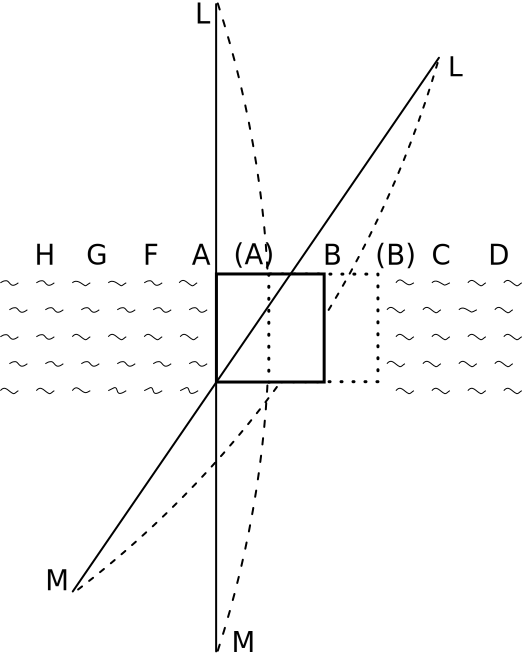
\includegraphics[width=0.89\textwidth]{gesamttex/edit_VIII,3/images/LH_37_01_001-002,003-008,025_d1a.pdf}
\end{minipage}
\hspace{11.5mm}
\begin{minipage}[t]{0.5\textwidth}
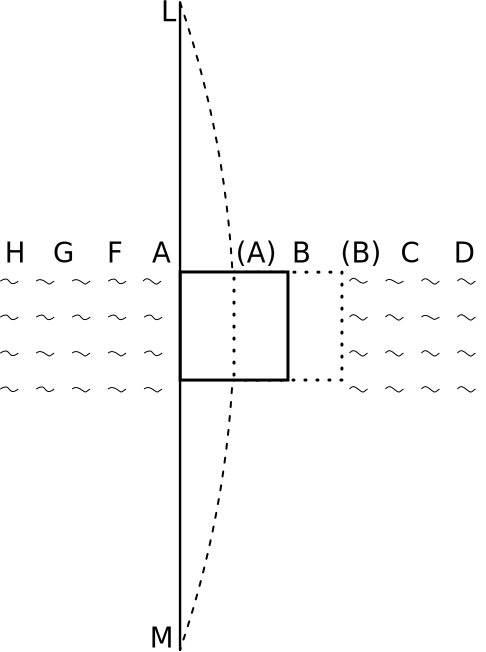
\includegraphics[width=0.79\textwidth]{gesamttex/edit_VIII,3/images/LH_37_01_001-002,003-008,025_d1b.pdf}
\end{minipage}
\\
\vspace{0.4em}
\newline \setline{4}
\hspace*{11mm} [\textit{Fig.~1a; L\textsuperscript{1}\! (Bl.~2~r\textsuperscript{o}\!)}\label{LH_37_01_002r_a1}]\hspace*{41mm} [\textit{Fig.~1b; Lil (Bl.~5~v\textsuperscript{o}\!)}\label{LH_37_01_005v_a1}]
\pend
\newpage
%%%%%%%%%%%%%%%%%%%%%%%%%%%%%%%%%%%%%%%%%%%%%%%%%%%%
%%\vspace*{1.5em}%
%  \centerline{\hspace*{-70mm}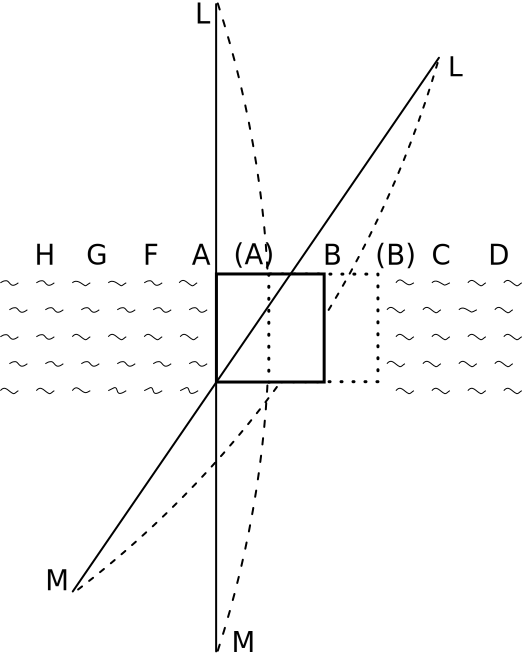
\includegraphics[width=0.46\textwidth]{gesamttex/edit_VIII,3/images/LH_37_01_001-002,003-008,025_d1a.pdf}}%\\
%  \vspace*{0.5em}% \vspace*{-1.5em}
%  \centerline{\hspace*{-70mm}\lbrack\textit{Fig.~1a; L\textsuperscript{1}\! (Bl.~2~r\textsuperscript{o}\!)}\rbrack}\label{LH_37_01_002r_a1}% \hspace*{-25mm}
%%  \vspace*{1.2em}%
%%  \newpage
%%
%%
%%
%%
%  \vspace*{-19.0em}%
%  \centerline{\hspace*{65mm}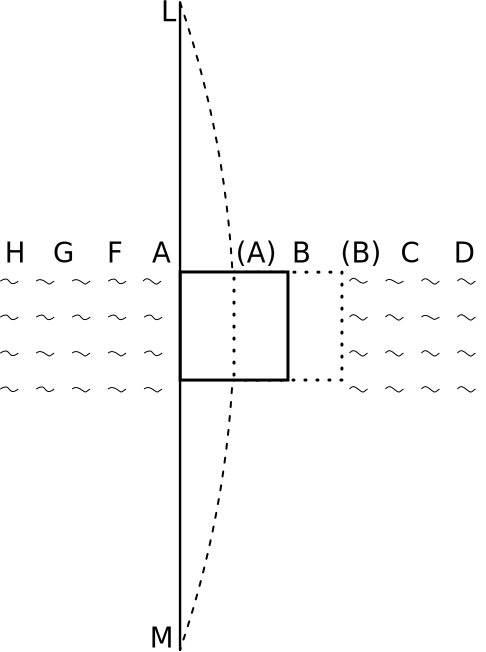
\includegraphics[width=0.42\textwidth]{gesamttex/edit_VIII,3/images/LH_37_01_001-002,003-008,025_d1b.pdf}}%\\
%  \vspace*{0.5em}% \vspace*{-1.5em}
%  \centerline{\hspace*{65mm}\lbrack\textit{Fig.~1b; Lil (Bl.~5~v\textsuperscript{o}\!)}\rbrack}\label{LH_37_01_005v_a1}% \hspace*{95mm}
%%  \vspace*{1.5em}%
%\newpage
%
%%
\count\Bfootins=1000
\count\Afootins=1200
\count\Cfootins=1200
\pstart
\noindent
portione  intelligentur. Modus quo sonus\protect\index{Sachverzeichnis}{propagatio soni} in aere\protect\index{Sachverzeichnis}{aer}
\edtext{propagetur nunquam}{%
\lemma{propagetur}\Bfootnote{% \hspace{-0.5mm}%
\lbrack2~r\textsuperscript{o}\rbrack\ nunquam% %%%% Blatt 2r
~\textit{L\textsuperscript{1}}}}
%
quod sciam satis explicatus est.
Circulos
\edtext{aqueis\protect\index{Sachverzeichnis}{circulus aqueus} similes,}{%
\lemma{aqueis}\Bfootnote{%
\hspace{-0.5mm}similes,
\textit{fehlt~\textit{L\textsuperscript{1}}, erg.~Lil}}}
%
\edtext{supra}{%
\lemma{supra}%
\Cfootnote{S.~\refpassage{LH_37_01_003r_caqs1}{LH_37_01_003r_caqs2}.}}
%
rejecimus,
nec putandum est opus
\edtext{esse}{%
\lemma{esse~,~\textit{L\textsuperscript{1}}}\Bfootnote{%
esse~\textit{l}}}
%
ut
\edtext{quasi sagittulae quaedam aereae\protect\index{Sachverzeichnis}{sagittula aerea}
a sonante\protect\index{Sachverzeichnis}{sonans} spargantur,}{%
\lemma{quasi \lbrack...\rbrack\ spargantur}\Cfootnote{%
Siehe \cite{00044}\textsc{Fabri}, \textit{Physica}, tract.~III, lib.~II, prop.~52 (Bd.~II, S.~145a).}}
%
\edtext{itaque utile erit aliquam figuram\protect\index{Sachverzeichnis}{figura} adhibere}{%
\lemma{itaque}\Bfootnote{%
\textit{(1)}~opus est aliqua figura
\textit{(2)}~utile erit aliquam figuram adhibere%
~\textit{L\textsuperscript{1}}}}
%
ad faciliorem rei novae intellectum.\protect\index{Sachverzeichnis}{intellectus}%
\pend
\pstart%
Sit\label{LH_37_01_005v_aac}\edlabel{LH_37_01_005v_aerconcurrens_jksdfsfdfo-1}
chorda $LAM$\protect\index{Sachverzeichnis}{chorda tensa}
\edtext{tensa per se,
inque duobus extremis fixis $LM$ firmata}{%
\lemma{tensa}\Bfootnote{\hspace{-0.5mm}%
\textbar~per se, \lbrack...\rbrack\ $LM$ firmata \textit{erg.}~\textbar~,%
~\textit{L\textsuperscript{1}}%
\hspace{0.5mm}
tensa per \lbrack...\rbrack\ $LM$ firmata% se,
~\textit{l}}}%
\lbrack,\rbrack\
%
ea in medio puncto $A$ apprehensa pulsetur,\protect\index{Sachverzeichnis}{chorda pulsata}
\edtext{seu ex linea}{%
\lemma{seu}\Bfootnote{\hspace{-0.5mm}%
a linea%
~\textit{L\textsuperscript{1}}%
\hspace{0.5mm}
seu
\textbar~ex \textit{erg.~Lil}~%
\textbar\ linea
~\textit{l}}}
%
recta $LM$ producatur in arcum\protect\index{Sachverzeichnis}{arcus}
\edtext{\textit{L(A)M}, et ultra; inde}{%
\lemma{\textit{L(A)M}}\Bfootnote{\hspace{-0.5mm}%
\textbar~et ultra \textit{erg.}~%
\textbar\ inde%
~\textit{L\textsuperscript{1}}%
\hspace{0.5mm}
\textit{L(A)M}~, et ultra; inde%
~\textit{l}}}
%
dimissa\protect\index{Sachverzeichnis}{chorda dimissa} sibi relinquatur,
ut redire ad priorem statum,\protect\index{Sachverzeichnis}{status prior}
quin et in contrariam partem versus $F$ deinde
\edtext{evagari}{%
\lemma{evagari~,~\textit{L\textsuperscript{1}}}\Bfootnote{%
evagari%
~\textit{l}}}
%
atque aliquamdiu
\edtext{motum}{%
\lemma{motum}\Bfootnote{\hspace{-0.5mm}%
\textit{erg.~L\textsuperscript{1}}}}
%
reciprocare possit.\protect\index{Sachverzeichnis}{motus reciprocationis}
Cum igitur
durante hac
\edtext{reciprocatione\protect\index{Sachverzeichnis}{reciprocatio chordae}}{%
\lemma{reciprocatione~,~\textit{L\textsuperscript{1}}}\Bfootnote{%
reciprocatione~\textit{l}}}
%
sonoque\protect\index{Sachverzeichnis}{ortus soni} inde
\edtext{orto,}{%
\lemma{orto~\textit{L\textsuperscript{1}}}\Bfootnote{%
orto~,~\textit{l}}}
%
rursus excurrit ab $A$
\edtext{in \textit{(A)},
tum ponamus facilioris ratiocinationis\protect\index{Sachverzeichnis}{ratiocinatio} causa
in puncto $A$ alligatum vel affixum chordae esse corpus $AB$\protect\index{Sachverzeichnis}{corpus affixum}
(\phantom)\hspace{-1.2mm}:~%
quale corpus ipsa chordae materia\protect\index{Sachverzeichnis}{materia chordae}
ad punctum $A$ ab uno latere chordae existens intelligi potest~:%
\phantom(\hspace{-1.2mm})%
}{%
\lemma{in}\Bfootnote{\hspace{-0.5mm}%
\textit{(A)},
\textit{(1)}~intelligamus in
\textit{(a)}~$A$ affix
\textit{(b)}~puncto $A$
\textit{(2)}~tum ponamus facilitatis causa
\textit{(a)}~in $A$ alligatum
\textit{(b)}~in puncto $A$ % alligatum vel affixum chordae esse 
\lbrack...\rbrack\ corpus $AB$
\textit{(aa)}~(\phantom)\hspace{-1.2mm}chordae partem si placet repraesentari\phantom(\hspace{-1.2mm})
\textit{(bb)}~(\phantom)\hspace{-1.2mm}quale corpus
\textit{(aaa)}~est
\textit{(bbb)}~ipsa chordae \lbrack...\rbrack\ punctum $A$ ab
\textit{(aaaa)}~una parte
\textit{(bbbb)}~uno latere \lbrack...\rbrack\ intelligi potest\phantom(\hspace{-1.2mm}),%
~\textit{L\textsuperscript{1}}%
\hspace{0.5mm}
in \textit{(A)}, tum ponamus
\textit{(1)}~facilitatis~\textit{l}
\textit{(2)}~facilioris ratiocinationis~\textit{Lil}
causa in % \lbrack...\rbrack\ corpus $AB$ (\phantom)\hspace*{-1.2mm}:~quale 
\lbrack...\rbrack\ ad punctum
\textit{(a)}~ab~\textit{l}
\textit{(b)}~$A$ ab~\textit{Lil}
uno latere \lbrack...\rbrack\ intelligi potest~:% chordae existens
\phantom(\hspace{-1.2mm})%
~\textit{l}}}
%
quod per vibrationem\protect\index{Sachverzeichnis}{vibratio chordae} ex
\edtext{loco $AB,$ transferatur in locum \textit{(A)(B)},
itaque aerem\protect\index{Sachverzeichnis}{aer expulsus} expellet ex loco \textit{B(B)}
quem corpus $AB$ nunc nove ingreditur,
et contra aerem alium faciet succedere
in locum \textit{A(A)} quem deserit.\protect\index{Sachverzeichnis}{locus aere desertus}
Sed cum vibratio\protect\index{Sachverzeichnis}{vibratio celerrima} sit celerrima
nec satis celeriter circulus aeris\protect\index{Sachverzeichnis}{circulus aeris} absolvi,
aerque ex \textit{B(B)} expulsus\protect\index{Sachverzeichnis}{aer expulsus} in spatio circumfuso aequaliter distribui possit;%
}{%
\lemma{loco}\Bfootnote{\hspace{-0.5mm}%
$AB,$
\textit{(1)}~transfertur
\textit{(2)}~transferatur in locum \textit{(A)(B)}
\textit{(a)}~cumque vibratio sit celerrima aer
\textit{(b)}~itaque aerem expellet ex loco \textit{B(B)}
\textit{(aa)}~quod
\textit{(bb)}~quem
\textit{(aaa)}~nunc in
\textit{(bbb)}~corpus $AB$ nunc
\textit{(aaaa)}~ingreditur, ex
\textit{(bbbb)}~nove ingreditur, \lbrack...\rbrack\ absolvi, aerque
\textit{(aaaaa)}~qui
\textit{(bbbbb)}~praecise sese aequaliter
\textit{(ccccc)}~ex \textit{B(B)} expulsus
\textit{(aaaaa-a)}~se aequaliter distribuere, et in
\textit{(bbbbb-b)}~in spatio circumfuso aequaliter
\textit{(aaaaa-aa)}~distribuere
\textit{(bbbbb-bb)}~distribui possit,%
~\textit{L\textsuperscript{1}}%
\hspace{0.5mm}
\mbox{loco} $AB,$ transferatur \lbrack...\rbrack\ distribui possit;%
~\textit{l}}}
%
hinc fit ut aer \textit{(B)C},
\edtext{anterior\protect\index{Sachverzeichnis}{aer compressus} corpore moto,
per istum impetum\protect\index{Sachverzeichnis}{impetus corporis moti} nonnihil comprimatur,}{%
\lemma{anterior}\Bfootnote{\hspace{-0.5mm}%
\textit{(1)}~sit impetu isto
\textit{(2)}~corpore moto \lbrack...\rbrack\ nonnihil comprimatur,% per istum impetum
~\textit{L\textsuperscript{1}}%
\hspace{0.5mm}
anterior corpore
\textit{(1)}~motus,~\textit{l}
\textit{(2)}~moto,~\textit{Lil}
per istum impetum nonnihil comprimatur,%
~\textit{l}}}
%
seu plus aeris\protect\index{Sachverzeichnis}{aer expulsus} expulsi accipiat quam alius remotior $CD.$
Et
\edtext{contra,}{%
\lemma{contra~\textit{L\textsuperscript{1}}}\Bfootnote{%
contra~,~\textit{l}}}
%
\edlabel{LH_37_01_005v_kfkskjll-1}%
\edtext{cum}{%
\lemma{cum}\Bfootnote{\hspace{-0.5mm}%
\textit{erg.~L\textsuperscript{1}}}}
%
aeri $AF$ qui posterior est
\edtext{corpore moto,}{%
\lemma{corpore}\Bfootnote{% \hspace{-0.5mm}%
\textit{(1)}~, cui
\textit{(2)}~moto,%
~\textit{L\textsuperscript{1}}}}
%
non
\edtext{tantum novi aeris\protect\index{Sachverzeichnis}{aer novus}
statim subministratur
quantum opus esset}{%
\lemma{tantum}\Bfootnote{\hspace{-0.5mm}%
\textit{(1)}~ipsi
\textit{(2)}~novi aeris statim 
\textit{(a)}~subministretur
\textit{(b)}~subministratur quantum 
\textit{(aa)}~ipse
\textit{(bb)}~opus
\textit{(aaa)}~est
\textit{(bbb)}~esset%
~\textit{L\textsuperscript{1}}%
\hspace{0.5mm}
tantum novi
\textit{(1)}~aliis~\textit{l}
\textit{(2)}~aeris~\textit{Lil}
statim subministratur quantum opus esset%
~\textit{l}}}
%
ad locum vacuum\protect\index{Sachverzeichnis}{locus vacuus} \textit{A(A)}
a corpore
\edtext{desertum,\protect\index{Sachverzeichnis}{locus a corpore desertus}}{%
\lemma{desertum~\textit{L\textsuperscript{1}}}\Bfootnote{%
desertum~,~\textit{l}}}
%
sine
\edtext{rarefactione\protect\index{Sachverzeichnis}{rarefactio}
implendum,\protect\index{Sachverzeichnis}{locus implendus}}{%
\lemma{rarefactione}\Bfootnote{\hspace{-0.5mm}%
\textbar~sui \textit{gestr.}~\textbar\ implendum,~\textit{L\textsuperscript{1}}}}
%
ideo ipse aer $AF$ nonnihil dilatatur,
eoque magis quo ipsi $A$ est propior\lbrack;\rbrack\
\edtext{itaque necesse est}{%
\lemma{itaque}\Bfootnote{\hspace{-0.5mm}%
\textit{(1)}~videmus quando
\textit{(2)}~necesse est%
~\textit{L\textsuperscript{1}}}}
%
aerem sonanti propinquum\protect\index{Sachverzeichnis}{aer sonanti propinquus}
comprimi\protect\index{Sachverzeichnis}{aer compressus} ac dilatari,\protect\index{Sachverzeichnis}{aer dilatatus}
sive
(\phantom)\hspace{-1.2mm}quia Tensionis\protect\index{Sachverzeichnis}{tensio} nomine
omnem corporis Elastici\protect\index{Sachverzeichnis}{corpus elasticum}
a naturali statu\protect\index{Sachverzeichnis}{status naturalis} dimotionem
\edtext{intelligo\phantom(\hspace{-1.2mm})
praeter solitum\textso{ tendi.}}{%
\lemma{intelligo\phantom(\hspace{-1.2mm})}\Bfootnote{\hspace{-0.5mm}%
\textit{(1)}~\textso{tendi}
\textit{(2)}~praeter solitum \textso{tendi.}%
~\textit{L\textsuperscript{1}}}}%
\edlabel{LH_37_01_005v_kfkskjll-2}
%
\edlabel{LH_37_01_005v_jgfxqmhrwt}%
Habet autem aer\protect\index{Sachverzeichnis}{aer tensus}\protect\index{Sachverzeichnis}{elastrum aeris}
suum jam Elastrum
\edtext{naturale\protect\index{Sachverzeichnis}{elastrum naturale}
determinatumque compressionis gradum,\protect\index{Sachverzeichnis}{gradus compressionis}
quem partim a sua natura\protect\index{Sachverzeichnis}{natura aeris}
partim ab incumbentis aeris pondere\protect\index{Sachverzeichnis}{pondus aeris} accepit;}{%
\lemma{naturale}\Bfootnote{\hspace{-0.5mm}%
\textit{(1)}~quem a
\textit{(2)}~determinatumque compressionis gradum, quem
\textit{(a)}~a pondere
\textit{(b)}~partim a \lbrack...\rbrack\ pondere accepit,%
~\textit{L\textsuperscript{1}}%
\hspace{0.5mm}
naturale determinatumque \lbrack...\rbrack\ pondere accepit;%
~\textit{l}}}
%
et
\edtext{omne elasticum\protect\index{Sachverzeichnis}{corpus elasticum}}{%
\lemma{omne}\Bfootnote{% \hspace{-0.5mm}%
Elasticum%
~\textit{L\textsuperscript{1}}%
\hspace{0.5mm}
omne elasticum%
~\textit{l}}}
%
sive tensum\protect\index{Sachverzeichnis}{corpus tensum}
\edtext{corpus,}{%
\lemma{corpus~\textit{L\textsuperscript{1}}}\Bfootnote{%
corpus~,~\textit{l}}}
%
cum majorem solito tensionem\protect\index{Sachverzeichnis}{tensio corporis elastici}
\edtext{accipit}{%
\lemma{accipit~,~\textit{L\textsuperscript{1}}}\Bfootnote{%
accipit~\textit{l}}}
%
sive cum
\edtext{pulsatur, tremit;}{%
\lemma{pulsatur}\Bfootnote{% \hspace{-0.5mm}%
tremit,%
~\textit{L\textsuperscript{1}}%
\hspace{0.5mm}
pulsatur~, tremit;%
~\textit{l}}}
%
aeris ergo portio\protect\index{Sachverzeichnis}{portio aeris} chordae
\edtext{propinqua, ipsamet}{%
\lemma{propinqua}\Bfootnote{\hspace{-0.5mm}%
\textbar~ipsamet \textit{erg.}~\textbar%
~\textit{L\textsuperscript{1}}%
\hspace{0.5mm}
propinqua~, ipsamet%
~\textit{l}}}
%
instar chordae\protect\index{Sachverzeichnis}{chorda tremens}
\edtext{alicujus}{%
\lemma{alicujus~,~\textit{L\textsuperscript{1}}}\Bfootnote{%
alicujus~\textit{l}}}
%
\edtext{tremit.
Et hunc
%
\lbrack6~r\textsuperscript{o}\rbrack\ %%%% Blatt 6r
%
tremorem\protect\index{Sachverzeichnis}{tremor aeris} continuaret aliquandiu}{%
\lemma{tremit.}\Bfootnote{\hspace{-0.5mm}%
\textit{(1)}~Cui accedit q
\textit{(2)}~Et hoc faceret
\textit{(3)}~Et hunc tremorem continuaret aliquandiu%
~\textit{L\textsuperscript{1}}}}
%
etsi non alius aer ipsi esset
\edtext{vicinus.\protect\index{Sachverzeichnis}{aer vicinus}
Veruntamen adhuc praeterea}{%
\lemma{vicinus.}\Bfootnote{\hspace{-0.5mm}%
\textit{(1)}~Sed tamen
\textit{(2)}~Veruntamen adhuc praeterea%
~\textit{L\textsuperscript{1}}}}
%
accedit nova causa\protect\index{Sachverzeichnis}{causa tremoris}
ab aere quoque
\edtext{vicino\protect\index{Sachverzeichnis}{aer vicinus}%
\lbrack,\rbrack\
quae continuationem auget.\protect\index{Sachverzeichnis}{continuatio tremoris}}{%
\lemma{vicino}\Bfootnote{\hspace{-0.5mm}%
\textbar~, quae continuationem auget \textit{erg.}~%
\textbar~.%
~\textit{L\textsuperscript{1}}%
\hspace{0.5mm}
vicino quae continuationem auget.%
~\textit{l}}}
%
Nam ut
\edtext{aer \textit{(B)C}}{%
\lemma{aer}\Bfootnote{\hspace{-0.5mm}%
\textit{(1)}~$BC$
\textit{(2)}~\textit{(B)C}%
~\textit{L\textsuperscript{1}}}}
%
justo compressior\protect\index{Sachverzeichnis}{aer compressus}
sese exonerare
\edtext{conatur in ambientem\lbrack,\rbrack\
ita contra ambiens aer\protect\index{Sachverzeichnis}{aer ambiens}}{%
\lemma{conatur}\Bfootnote{\hspace{-0.5mm}%
in
\textit{(1)}~vicinum,
\textit{(2)}~ambientem, ita contra
\textit{(a)}~vicinus
\textit{(b)}~ambiens%
~\textit{L\textsuperscript{1}}}}
%
magna vi\protect\index{Sachverzeichnis}{vis magna} irruit in locum aeris \textit{F(A)}
\edtext{justo dilatatioris:\protect\index{Sachverzeichnis}{aer dilatatus} sed aer
se exonerans, sese justo amplius exonerat;
et contra, aer irruens,\protect\index{Sachverzeichnis}{aer irruens} justo largius irruit;
uti pendulum\protect\index{Sachverzeichnis}{pendulum} descendendo exorbitat,
justoque longius movetur atque \lbrack iterum\rbrack\ ascendit;
unde}{%
\lemma{justo}\Bfootnote{\hspace{-0.5mm}%
dilatatioris.
\textit{(1)}~Unde
\textit{(2)}~Sed aer
\textbar~partim \textit{gestr.}~%
\textbar\ se exonerans, \lbrack...\rbrack\ exonerat, et contra aer irruens justo largius irruit, % sese justo amplius  
\textit{(a)}~unde
\textit{(b)}~uti pendulum
\textit{(aa)}~post descensum justo longius
\textit{(bb)}~descendendo exorbitat justoque longius movetur,
\textit{(aaa)}~iterumque
\textit{(bbb)}~atque iterum ascendit. Unde%
~\textit{L\textsuperscript{1}}%
\hspace{0.5mm}
justo
\textit{(1)}~dilatioris. Sed aer~\textit{l}
\textit{(2)}~dilatatioris: sed aer~\textit{Lil}
se exonerans, \lbrack...\rbrack\ movetur atque
\textbar~iterumque \textit{ändert Hrsg. nach L\textsuperscript{1}}
\textbar\ ascendit; unde%
~\textit{l}}}%
%%%%
%%%%
\edlabel{KZeitz35}\edtext{}{{\xxref{KZeitz35}{KZeitz36}}%
{%
\lemma{vibratio}\Bfootnote{\hspace{-0.5mm}%
\textbar~%
\textit{(1)}~aliquandiu
\textit{(2)}~satis diu
\textit{erg.}~\textbar\
continuata.
\textit{(1)}~Sciendum est \textbar~quoque \textit{erg.}~\textbar\ portionem aeris ut $AF$ dum vibrationes suas exercet,
\textit{(a)}~divelli ab alia
\textit{(b)}~quodammodo \textbar~recedentem \textit{erg.}~\textbar\ distrahi ab alia parte aeris vicini $FG$
\textit{(aa)}~et rursus
\textit{(bb)}~eamque
\textit{(aaa)}~tendere
\textit{(bbb)}~dilatare et diducere, et contra rursus \textbar~eam comprimere \textit{erg.}~\textbar\ accedentem
\textit{(aaaa)}~neque enim
\textit{(bbbb)}~unde in loco intercepto nova rursus dilatatio
\textit{(aaaaa)}~et \textbar~postea \textit{erg.}~\textbar\ compressio reciprocata, seu vibratio
\textit{(bbbbb)}~, \textbar~quam sequitur nimia restitutio \textit{erg.}~\textbar\ seu compressio et ex his reciprocatis vibratio.
\textit{(2)}~Aer jam vibrans \textbar~\textit{(B)C} \textit{erg.}~\textbar~, vicinum quoque \textbar~sibi \textit{erg.}~\textbar\ aerem
\textit{(a)}~commovet
\textit{(b)}~sed a corpore sonante longius remotum, % corpore sonante
\textbar~in \textit{versehentlich erhalten}~%
\textbar\ commovet ad vibrandum; \lbrack...\rbrack\ etiam cum
\textit{(aa)}~reversus
\textit{(bb)}~justo amplius \lbrack...\rbrack\ sese contrahens
\textit{(aaa)}~ab eo distrahitur
\textit{(bbb)}~ab altero
\lbrack...\rbrack\ \textit{(A)(B)} vacuefactum replere conatur,
\lbrack...\rbrack\ a vicino $GH$ unde
\lbrack...\rbrack\ seu compressio et utriusque
\lbrack...\rbrack\ quomodo aer
\textbar~\textit{(B)C} vel $AF$ \textit{erg.}~%
\textbar\ tam dilatans \lbrack...\rbrack\ in vicinum,
\textit{(aaaa)}~quam
\textit{(bbbb)}~postquam a corpore vibrante
\textit{(aaaaa)}~compressus est, quam distrahens
\textit{(bbbbb)}~propulsus aut
\lbrack...\rbrack\ compressus est; quam contrahens
\lbrack...\rbrack\ a vicino, postquam a corpore vibrante attractus,
\lbrack...\rbrack\ dilatatus est, vicinum ut \textit{(B)C} ipsum $CD$ et $AF$ ipsum $FG$
\textit{(aaaaa-a)}~pulset
\textit{(bbbbb-b)}~comprimat vel diducat adeoque pulset sive tendat et
\lbrack...\rbrack\ vibrandum commoveat.%
~\textit{L\textsuperscript{1}}%
\hspace{0.5mm}
%%%%
vibratio
\textit{(1)}~satis diu continuata.~\textit{l}
\textit{(2)}~nascitur aliquandiu duratura.~\textit{Lil}
Aer jam \lbrack...\rbrack\ aerem, sed
\textit{(a)}~in~\textit{l}
\textit{(b)}~a~\textit{Lil}
corpore sonante \lbrack...\rbrack\ aer \textit{(B)C} vel $AF$
\textit{(aa)}~dilatans~\textit{l}
\textit{(bb)}~tam dilatans~\textit{Lil}
sese seu exonerans in vicinum
\textit{(aaa)}~,~\textit{l}
\textit{(bbb)}~(\phantom)\hspace{-1.2mm}:~\textit{Lil}
postquam a \lbrack...\rbrack\ compressus est
\textit{(aaaa)}~;~\textit{l}
\textit{(bbbb)}~:\phantom(\hspace{-1.2mm})~\textit{Lil}
quam contrahens % sese seu distrahens
\lbrack...\rbrack\ a vicino 
\textbar~(\phantom)\hspace{-1.2mm}: \textit{erg.~Lil}~%
\textbar\ postquam a % corpore vibrante
\lbrack...\rbrack\ dilatatus est
\textbar~:\phantom(\hspace{-1.2mm}) \textit{erg.~Lil}~%
\textbar\ vicinum % \textit{l}
\textbar~(\phantom)\hspace{-1.2mm}: \textit{erg.~Lil}~%
\textbar\ ut % \textit{l}
\textbar~aer \textit{erg.~Lil}~%
\textbar\ \textit{(B)C} ipsum $CD$ et % \textit{l}
\textbar~aer \textit{erg.~Lil}~%
\textbar\ $AF$ ipsum $FG$ % \textit{l}
\textbar~:\phantom(\hspace{-1.2mm}) \textit{erg.~Lil}~%
\textbar\ comprimat vel % diducat, adeoque pulset vel
\lbrack...\rbrack\  tendat et
\textbar~ad \textit{erg.~Lil}~%
\textbar\ similiter vibrandum commoveat.%
~\textit{l}}}}
vibratio\protect\index{Sachverzeichnis}{vibratio aeris} nascitur aliquandiu duratura.
Aer jam vibrans\protect\index{Sachverzeichnis}{aer vibrans} \textit{(B)C} vicinum quoque sibi aerem,\protect\index{Sachverzeichnis}{aer vicinus}
sed a corpore sonante\protect\index{Sachverzeichnis}{corpus sonans} longius remotum,
commovet ad vibrandum,
non tantum cum in ipsum irruit\protect\index{Sachverzeichnis}{aer irruens} et exonerare se conatur,
sed etiam cum justo amplius dilatatus\protect\index{Sachverzeichnis}{aer dilatatus} iterum redit ad se
et sese contrahens\protect\index{Sachverzeichnis}{aer contractus} ab altero distrahitur.\protect\index{Sachverzeichnis}{aer distractus}
Quod et de aere $AF$ dicendum est,
qui dum locum \textit{A(A)} corporis $AB$ transitu in \textit{(A)(B)} vacuefactum,\protect\index{Sachverzeichnis}{locus vacuefactus}
replere conatur,
ut \edtext{supra}{\lemma{supra}\Cfootnote{S.~\refpassage{LH_37_01_005v_kfkskjll-1}{LH_37_01_005v_kfkskjll-2}.}}
diximus\lbrack,\rbrack\
et versus \textit{A(A)} tendit,
quodammodo distrahitur a vicino $GH,$\protect\index{Sachverzeichnis}{aer distractus}
unde aer interceptus\protect\index{Sachverzeichnis}{aer interceptus} $FG$
tenditur\protect\index{Sachverzeichnis}{aer tensus} ac dilatatur\lbrack;\rbrack\
quam dilatationem\protect\index{Sachverzeichnis}{dilatatio aeris}
sequitur restitutio\protect\index{Sachverzeichnis}{restitutio aeris} nimia
seu compressio,\protect\index{Sachverzeichnis}{compressio aeris}
et utriusque reciprocatio\protect\index{Sachverzeichnis}{reciprocatio aeris}
seu vibratio.\protect\index{Sachverzeichnis}{vibratio aeris}
Habemus ergo quomodo aer \textit{(B)C} vel $AF$ tam dilatans sese
seu exonerans in vicinum\protect\index{Sachverzeichnis}{aer vicinus}
(\phantom)\hspace{-1.2mm}:~%
postquam a corpore vibrante\protect\index{Sachverzeichnis}{corpus vibrans} propulsus
aut propriae restitutionis nisu\protect\index{Sachverzeichnis}{nisus restitutionis}
nimium compressus\protect\index{Sachverzeichnis}{aer compressus} est~%
:\phantom(\hspace{-1.2mm})
quam contrahens\protect\index{Sachverzeichnis}{aer contractus} sese
seu distrahens\protect\index{Sachverzeichnis}{aer distractus} a vicino\protect\index{Sachverzeichnis}{aer vicinus}
(\phantom)\hspace{-1.2mm}:~%
postquam a corpore vibrante\protect\index{Sachverzeichnis}{corpus vibrans}
attractus\protect\index{Sachverzeichnis}{aer attractus}
aut propriae restitutionis nisu\protect\index{Sachverzeichnis}{nisus restitutionis}
nimium dilatatus\protect\index{Sachverzeichnis}{aer dilatatus} est~%
:\phantom(\hspace{-1.2mm})
vicinum
(\phantom)\hspace{-1.2mm}:~%
ut aer \textit{(B)C} ipsum $CD$ et aer $AF$ ipsum $FG$~%
:\phantom(\hspace{-1.2mm})
comprimat vel diducat,\protect\index{Sachverzeichnis}{aer diductus}
adeoque pulset\protect\index{Sachverzeichnis}{aer pulsatus}
vel tendat\protect\index{Sachverzeichnis}{aer tensus}
et ad similiter vibrandum\protect\index{Sachverzeichnis}{aer vibrans} commoveat.\edlabel{KZeitz36}
%%%%
%%%%
Atque ita propagatur et vibratio\protect\index{Sachverzeichnis}{vibratio aeris} ab aere $AF$ ad vicinum $FG,$
et ab hoc similiter ad vicinum\protect\index{Sachverzeichnis}{aer vicinus}
\edtext{$GH$ et ita porro;}{%
\lemma{$GH$}\Bfootnote{\hspace{-0.5mm}%
\textbar~et ita porro: \textit{erg.}~\textbar%
~\textit{L\textsuperscript{1}}%
\hspace{0.5mm}
$GH$ et ita porro;%
~\textit{l}}}
%
perinde ac si imaginaremur plures chordas
\edtext{$LM,$ $NO,$ $PQ$}{%
\lemma{$LM,$ $NO,$ $PQ$}\Cfootnote{%
Siehe \lbrack\textit{Fig.~2}\rbrack.}}
sibi vicinas\protect\index{Sachverzeichnis}{chorda vicina}
\edtext{esse; unamque}{%
\lemma{esse}\Bfootnote{\hspace{-0.5mm}%
unam~\textit{L\textsuperscript{1}}%
\hspace{0.5mm}
esse~;
\textit{(1)}~unam~\textit{l}
\textit{(2)}~unamque%
~\textit{Lil}}}
%
$LM$ pulsatam\protect\index{Sachverzeichnis}{chorda pulsata}
vibrare\protect\index{Sachverzeichnis}{chorda vibrans} usque ad sequentem $NO,$
\edtext{quae hoc modo etiam pulsata\protect\index{Sachverzeichnis}{chorda pulsata}
pulset}{%
\lemma{quae}\Bfootnote{\hspace{-0.5mm}%
\textit{(1)}~iterum
\textit{(2)}~hoc modo etiam pulsata
\textit{(a)}~est
\textit{(b)}~, pulsat%
~\textit{L\textsuperscript{1}}%
\hspace{0.5mm}
quae hoc \lbrack...\rbrack\ pulsata pulset% modo etiam
~\textit{l}}}
%
rursus sequentem $PQ$ atque ita porro,
quousque continuantur chordae,
donec paulatim
\edtext{in postremis chordis}{%
\lemma{in}\Bfootnote{\hspace{-0.5mm}%
postremis chordis
\textit{erg.~L\textsuperscript{1}}}}
%
frangatur pulsandi impetus\protect\index{Sachverzeichnis}{impetus pulsandi}
excursionesque\protect\index{Sachverzeichnis}{excursio chordae}
\edtext{minuantur}{%
\lemma{minuantur~,~\textit{L\textsuperscript{1}}}\Bfootnote{%
minuantur~\textit{l}}}%
\lbrack,\rbrack\
%
ut chorda licet
\edtext{vibrata\protect\index{Sachverzeichnis}{chorda vibrans} sequentem non amplius attingat;
quod licet in aere\protect\index{Sachverzeichnis}{aer vibrans} non fiat}{%
\lemma{vibrata}\Bfootnote{\hspace{-0.5mm}%
\textit{(1)}~aliam insu
\textit{(2)}~sequentem non amplius attingat, quod
\textit{(a)}~tamen in aere non fiet
\textit{(b)}~licet in aere non fiat,%
~\textit{L\textsuperscript{1}}%
\hspace{0.5mm}
vibrata sequentem \lbrack...\rbrack\ non fiat% non amplius attingat; quod licet in aere
~\textit{l}}}
%
quia continuum est
\edtext{corpus,\protect\index{Sachverzeichnis}{corpus continuum}}{%
\lemma{corpus~\textit{L\textsuperscript{1}}}\Bfootnote{%
corpus~,%
~\textit{l}}}
%
vibrationes tamen
\edlabel{LH_37_01_006r_rsksaf-1}postremae\protect\index{Sachverzeichnis}{vibratio postrema}
imperceptibiles\protect\index{Sachverzeichnis}{vibratio imperceptibilis} fient
exiguosque nimis habebunt \protect\index{Sachverzeichnis}{excursus vibrationis}excursus\lbrack,\rbrack\
ac proinde cum idem fere tempus\protect\index{Sachverzeichnis}{tempus vibrationis}
semper etiam parvo excursu insumant,
motum habebunt tardissimum.\protect\index{Sachverzeichnis}{motus vibrationis}%
%
\edtext{}{%
{\xxref{LH_37_01_006r_rsksaf-1}{LH_37_01_006r_rsksaf-2}}%
{\lemma{postremae}\Bfootnote{\hspace{-0.5mm}%
\textit{(1)}~insensibiles fient\protect\index{Sachverzeichnis}{vibratio insensibilis}
\textit{(2)}~imperceptibiles fient
\textit{(a)}~. Haec jam
\textit{(b)}~exiguosque nimis habebunt excursus, \lbrack...\rbrack\ cum idem \textbar~fere \textit{erg.}~\textbar\ tempus semper parvo quoque excursu \lbrack...\rbrack\ pulsante illustrantur% aerem
~\textit{L\textsuperscript{1}}%
\hspace{0.5mm}
postremae imperceptibiles \lbrack...\rbrack\ tempus semper
\textit{(1)}~parvo quoque~\textit{l}
\textit{(2)}~etiam parvo~\textit{Lil}
excursu insumant, \lbrack...\rbrack\ aerem pulsante
\textbar~quae si promta sit aerem modo explicato pulsabit \textit{fehlt L\textsuperscript{1}, gestr.}~\textbar\ illustrantur%
~\textit{l}}}}
\pend
\pstart
Haec\edlabel{LH_37_01_006r_aerconcurrens-1} autem
quae
\edtext{diximus}{\lemma{diximus}\Cfootnote{% Siehe 
S.~\pageref{LH_37_01_005v_aac}\,ff.}}
de aere aerem\protect\index{Sachverzeichnis}{aer aerem pulsans}
pulsante illustrantur\edlabel{LH_37_01_006r_rsksaf-2}
non parum
\edtext{experimento\protect\index{Sachverzeichnis}{experimentum Gerickianum} vacui ab aere ordinario\protect\index{Sachverzeichnis}{aer ordinarius} loci.\protect\index{Sachverzeichnis}{locus vacuus}}{%
{\lemma{experimento}\Bfootnote{\hspace{-0.5mm}%
\textit{(1)}~Gerickiano
\textit{(2)}~vacuo
\textit{(3)}~vacui ab aere ordinario loci.%
~\textit{L\textsuperscript{1}}}}%
{\lemma{experimento \lbrack...\rbrack\ loci}\Cfootnote{%
Siehe \textsc{% O.~von
Guericke}, \textit{Experimenta nova}, l.~III, cap.~23\textendash25 % Amsterdam 1672, 
(S.~104\textendash107)\cite{00055}
sowie Leibnizens Auzüge hieraus (\textit{LSB} VIII,~1 N.~36, S.~258).\cite{01197}}}}
Nam
\edtext{quemadmodum}{%
\lemma{quemadmodum}\Bfootnote{\hspace{-0.5mm}%
\textit{fehlt~L\textsuperscript{1}, erg.~Lil}}}
 %
si duo hemisphaeria exhausta\protect\index{Sachverzeichnis}{hemisphaerium exhaustum} subito
\edtext{distrahantur}{%
\lemma{distrahantur~,~\textit{L\textsuperscript{1}}}\Bfootnote{%
distrahantur%
~\textit{l}}}
%
aerque
\edtext{ab omni parte}{%
\lemma{ab}\Bfootnote{\hspace{-0.5mm}%
\textit{(1)}~utraque
\textit{(2)}~omni parte
\textit{erg.~L\textsuperscript{1}}}}
%
magna vi\protect\index{Sachverzeichnis}{vis magna}
irruat,\protect\index{Sachverzeichnis}{aer irruens}
duo aeres concurrentes\protect\index{Sachverzeichnis}{aer aeri concurrens}
ingen-
% % % %    ACHTUNG GETRIXT: Die folgende Cfootnote hängt mit Fig. 2 zusammen.
\edtext{}{\lemma{\lbrack\textit{Fig.~2}\rbrack}\killnumber\Cfootnote{In \textit{L\textsuperscript{1}}\! (Bl.~2~r\textsuperscript{o}\!) liegt ein gestr. Entwurf dieses Diagramms vor.}}%
\pend%
%
%
%  \newpage
  \vspace{2.0em}%
  \centerline{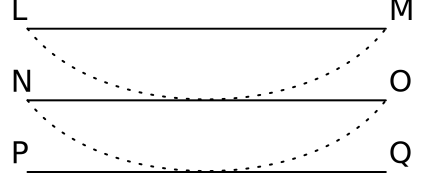
\includegraphics[width=0.37\textwidth]{gesamttex/edit_VIII,3/images/LH_37_01_001-002,003-008,025_d2.pdf}}%\\
  \vspace{1.5em}
  \centerline{\lbrack\textit{Fig.~2; L\textsuperscript{1}\! (Bl.~2~r\textsuperscript{o}\!) u. Lil (Bl.~6~r\textsuperscript{o}\!)}\rbrack}%
  \label{LH_37_01_005r_Fig.2}%
 % \vspace*{2.0em}%
%\newpage
%
%
\pstart%
\noindent
tem instar sclopeti\protect\index{Sachverzeichnis}{sclopetum}
\edtext{fragorem\protect\index{Sachverzeichnis}{fragor} edent, seu}{%
\lemma{fragorem}\Bfootnote{\hspace{-0.5mm}%
edunt
\textit{(1)}~;
\textit{(2)}~seu%
~\textit{L\textsuperscript{1}}%
\hspace{0.5mm}
fragorem edent, seu%
~\textit{l}}}
%
in partibus suis vicinisque
\edtext{tremorem\protect\index{Sachverzeichnis}{tremor aeris}
efficient; ita}{%
\lemma{tremorem}\Bfootnote{\hspace{-0.5mm}%
efficiunt. Ita%
~\textit{L\textsuperscript{1}}%
\hspace{0.5mm}
tremorem efficient
\textit{(1)}~.~Ita~\textit{l}
\textit{(2)}~;~ita%
~\textit{Lil}}}
%
hic quoque cum\lbrack,\rbrack\
\edtext{dilatato\protect\index{Sachverzeichnis}{aer dilatatus} partim,
partim compresso\protect\index{Sachverzeichnis}{aer compressus}
aere per sonori corporis\protect\index{Sachverzeichnis}{corpus sonorum}
vibrationem,\protect\index{Sachverzeichnis}{vibratio corporis}
%
\lbrack6~v\textsuperscript{o}\rbrack\ %%%% Blatt 6v
%
etiam oriatur aliquid vacui\protect\index{Sachverzeichnis}{locus vacuus}
id est loci aere valde exhausti,\protect\index{Sachverzeichnis}{locus aere exhaustus}
hinc etiam ex collisione\protect\index{Sachverzeichnis}{collisio aeris}
aeris irruentis\protect\index{Sachverzeichnis}{aer irruens}
in locum vacuum,\protect\index{Sachverzeichnis}{locus vacuus}
seu sese exonerantis ex compresso,\protect\index{Sachverzeichnis}{aer compressus}}{%
\lemma{dilatato}\Bfootnote{\hspace{-0.5mm}%
partim,
\textit{(1)}~partim
\textit{(2)}~aere
\textit{(3)}~partim compresso
\textit{(a)}~sonori ali
\textit{(b)}~aere \textbar~per \textit{erg.}~\textbar\ sonori corporis vibrationem, aliquis
\textit{(aa)}~sit
\textit{(bb)}~sit tum compressi aeris tum etiam vacui id est aeris exhausti gradus exiguus
\textit{(aaa)}~tamen aliquis
\textit{(bbb)}~licet, aliquis tamen
\textit{(aaaa)}~sit
\textit{(bbbb)}~hinc etiam
\textbar~ex collisione % aeris irruentis in locum vacuum, seu sese exonerantis 
\lbrack...\rbrack\ ex compresso \textit{erg.}~\textbar%
~\textit{L\textsuperscript{1}}%
\hspace{0.5mm}
dilatato partim,
\textbar~partim \textit{erg.~Lil}~%
\textbar\ compresso aere \lbrack...\rbrack\ corporis vibrationem, % per sonori
\textit{(1)}~aliquis sit tum \lbrack6~v\textsuperscript{o}\rbrack\ compressi aeris tum etiam~\textit{l}
\textit{(2)}~aliqui % \lbrack6~v\textsuperscript{o}\rbrack\ 
\textit{(3)}~etiam oriatur aliquid~\textit{Lil}
vacui id est
\textit{(a)}~aere\lbrack\textit{!}\rbrack\
 exhausti, gradus\protect\index{Sachverzeichnis}{gradus vacui} exiguus licet aliquis tamen~\textit{l}
\textit{(b)}~loci aere valde exhausti,~\textit{Lil}
hinc etiam \lbrack...\rbrack\
% ex collisione aeris
% \textit{(aa)}~irruentis~\textit{l}
% \textit{(bb)}~irruentis~\textit{Lil}
% in locum vacuum, seu sese exonerantis 
ex compresso,%
~\textit{l}}}
%
rudimentum aliquod
% \edtext{}{\lemma{rudimentum}\Bfootnote{%
% \textit{(1)}~aliquod~\textit{l}
% \textit{(2)}~aliquod~\textit{Lil}}}
soni\protect\index{Sachverzeichnis}{rudimentum soni}
seu
\edtext{tremorem\protect\index{Sachverzeichnis}{tremor aeris} et hujus aeris}{%
\lemma{tremorem}\Bfootnote{\hspace{-0.5mm}%
\textit{(1)}~aer
\textit{(2)}~et hujus aeris%
~\textit{L\textsuperscript{1}}}}
%
et
\edtext{vicini,\protect\index{Sachverzeichnis}{aer vicinus}}{%
\lemma{vicini~\textit{L\textsuperscript{1}}}\Bfootnote{%
vicini~,%
~\textit{l}}}
%
consequi necesse est.\edlabel{LH_37_01_006r_aerconcurrens-2}\edlabel{LH_37_01_006v_aerconcurrens_jksdfsfdfo-2}%
%
\edlabel{KZeitz37}\edtext{}{{\xxref{KZeitz37}{KZeitz38}}%
{%
\lemma{Hactenus}\Bfootnote{%
porro \lbrack...\rbrack\ corporis sonori
\textit{(1)}~itionem
\textit{(2)}~$AB$ itionem \lbrack...\rbrack\ promta sit aerem modo explicato pulsabit.
\textit{erg.~L\textsuperscript{1}}%
\hspace{0.5mm}
Hactenus porro \lbrack...\rbrack\ explicato pulsabit.%
~\textit{l}}}}
Hactenus porro unam tantum
\edtext{corporis sonori\protect\index{Sachverzeichnis}{corpus sonorum} $AB$}{%
\lemma{corporis sonori $AB$}\Cfootnote{%
Siehe \lbrack\textit{Fig.~1b}\rbrack\ auf S.~\pageref{LH_37_01_005v_a1}.}}
%
itionem spectavimus ab $AB$ in \textit{(A)(B)},
quae si promta sit,
aerem\protect\index{Sachverzeichnis}{aer pulsatus} modo explicato pulsabit.\edlabel{KZeitz38}
%
Atque aer quidem semel
\edtext{in motu reciproco\protect\index{Sachverzeichnis}{motus reciprocus aeris}}{%
\lemma{in}\Bfootnote{\hspace{-0.5mm}%
\textit{(1)}~vibratione
\textit{(2)}~motu reciproco%
~\textit{L\textsuperscript{1}}}}
%
positus aliquandiu vibrationes\protect\index{Sachverzeichnis}{vibratio aeris} continuaret
\edtext{ut ostendimus,}{%
{\lemma{ut}\Bfootnote{\hspace{-0.5mm}%
ostendimus
\textit{erg.~L\textsuperscript{1}}}}%
{\lemma{ut ostendimus}\Cfootnote{% Siehe 
S.~\refpassage{LH_37_01_005v_jgfxqmhrwt}{LH_37_01_005v_jgfxqmhrwt}\,ff.}}}
%
etsi chordam tensam\protect\index{Sachverzeichnis}{chorda tensa} statim post primam vibrationem requiescere
\edtext{fingeremus;}{%
\lemma{fingeremus~,~\textit{L\textsuperscript{1}}}\Bfootnote{%
fingeremus~;%
~\textit{l}}}
%
tametsi hinc nullus
\edtext{fortasse}{%
\lemma{fortasse}\Bfootnote{\hspace{-0.5mm}%
\textit{erg.~L\textsuperscript{1}}}}
%
oriturus esset sonus,\protect\index{Sachverzeichnis}{ortus soni}
\edlabel{LH_37_01_006v_auditusutvisus-1}quemadmodum pauciores justo radii\protect\index{Sachverzeichnis}{radius}
non faciunt visum.\edlabel{LH_37_01_006v_auditusutvisus-2}\protect\index{Sachverzeichnis}{visus}
Verum nunc considerandum est corpus $AB$
cum excurrit in \textit{(A)(B)},
rursus regredi in locum $AB,$
imo transgredi in alteram partem versus $F,$
idque facere
\edtext{aliquoties; semper}{%
\lemma{aliquoties~.}\Bfootnote{\hspace{-0.5mm}%
Semper%
~\textit{L\textsuperscript{1}}%
\hspace{0.5mm}
aliquoties~; semper%
~\textit{l}}}
%
ergo novos vibrandi conatus\protect\index{Sachverzeichnis}{conatus vibrandi}
aeri ambienti\protect\index{Sachverzeichnis}{aer ambiens}
\edtext{imprimet.\protect\index{Sachverzeichnis}{conatus impressus}
Sed}{%
\lemma{imprimet.}\Bfootnote{\hspace{-0.5mm}%
\textit{(1)}~Verum
\textit{(2)}~Sed%
~\textit{L\textsuperscript{1}}}}
%
cum aer ille retineat adhuc vibrationes\protect\index{Sachverzeichnis}{vibratio aeris} a
\edtext{praecedentibus ejusdem chordae impressionibus\protect\index{Sachverzeichnis}{impressio chordae}
acceptas,\protect\index{Sachverzeichnis}{vibratio accepta}}{%
\lemma{praecedentibus}\Bfootnote{\hspace{-0.5mm}%
ejusdem chordae impressionibus acceptas,%
~\textit{L\textsuperscript{1}}%
\hspace{0.5mm}
praecedentibus
\textbar~et \textit{gestr.~Lil}~%
\textbar\ ejusdem chordae impressionibus
\textit{(1)}~\textlangle acce\textrangle ptas,~\textit{l}
\textit{(2)}~acceptas,%
~\textit{Lil}}}
%
hinc sequetur aliqua
\edtext{perturbatio:\protect\index{Sachverzeichnis}{perturbatio motus}
continget enim saepe ut vibrationes inter se non consentiant,}{%
\lemma{perturbatio~;}\Bfootnote{\hspace{-0.5mm}%
\textit{(1)}~fieri enim poterit ut aer
\textit{(2)}~fiet enim
\textit{(3)}~continget enim
\textbar~saepe \textit{erg.}~%
\textbar\ ut vibrationes
\textbar~inter se \textit{erg.}~%
\textbar\ non consentiant,%
~\textit{L\textsuperscript{1}}%
\hspace{0.5mm}
perturbatio~: continget \lbrack...\rbrack\ non consentiant,% enim saepe ut vibrationes inter se
~\textit{l}}}
%
dum enim nova chordae impressio\protect\index{Sachverzeichnis}{impressio chordae}
aerem forte solicitabit ad compressionem,\protect\index{Sachverzeichnis}{compressio aeris}
ipse ex prioris vibrationis reliquiis\protect\index{Sachverzeichnis}{reliquiae vibrationis}
tendet ad
\edtext{dilatationem\protect\index{Sachverzeichnis}{dilatatio aeris} % \lbrack,\rbrack\
vel contra.
Sed}{%
\lemma{dilatationem}\Bfootnote{\hspace{-0.5mm}%
\textbar~,~vel contra \textit{erg.}~\textbar~. Sed%
~\textit{L\textsuperscript{1}}%
\hspace{0.5mm}
dilatationem vel contra. Sed%
~\textit{l}}}
%
haec cum magnam factura sint motuum
\edtext{perturbationem\protect\index{Sachverzeichnis}{perturbatio motus}}{%
\lemma{perturbationem~,~\textit{L\textsuperscript{1}}}\Bfootnote{%
perturbationem%
~\textit{l}}}
%
et chorda\protect\index{Sachverzeichnis}{chorda vibrans}
\edtext{fortior praesenti vibratione
reliquiis prioris vibrationis\protect\index{Sachverzeichnis}{reliquiae vibrationis}
praevaleat,\protect\index{Sachverzeichnis}{vibratio praevalens}
sintque chordae vibrationes semper aequabiles\protect\index{Sachverzeichnis}{vibratio aequabilis}
et aequidiuturnae\protect\index{Sachverzeichnis}{vibratio aequidiuturna}%
}{%
\lemma{fortior}\Bfootnote{\hspace{-0.5mm}%
\textbar~praesenti vibratione reliquiis prioris \textit{erg.}~%
\textbar\ praevaleat,
\textbar~sintque ejus vibrationes semper aequabiles et aequidiuturnae \textit{erg.}~\textbar% semper aequabiles
~\textit{L\textsuperscript{1}}%
\hspace{0.5mm}
fortior praesenti vibratione reliquiis prioris 
\textbar~vibrationis \textit{erg.~Lil}~%
\textbar\ praevaleat, sintque
\textit{(1)}~ejus~\textit{l}
\textit{(2)}~chordae%
~\textit{Lil}
vibrationes semper aequabiles et aequidiuturnae%
~\textit{l}}}%
\lbrack,\rbrack\
%
hinc aer se paulatim ita chordae
\edtext{accommodat}{%
\lemma{accommodat~,~\textit{L\textsuperscript{1}}}\Bfootnote{%
accommodat%
~\textit{l}}}
%
ut
\edtext{mox}{%
\lemma{mox}\Bfootnote{\hspace{-0.5mm}%
\textit{erg.~L\textsuperscript{1}}}}
%
vibrationes aeris\protect\index{Sachverzeichnis}{vibratio aeris}
vibrationibus chordae\protect\index{Sachverzeichnis}{vibratio chordae}
\edtext{consentiant,\protect\index{Sachverzeichnis}{vibratio consentiens}
et}{%
\lemma{consentiant~;}\Bfootnote{\hspace{-0.5mm}%
\textit{(1)}~aut
\textit{(2)}~et%
~\textit{L\textsuperscript{1}}%
\hspace{0.5mm}
consentiant~, et%
~\textit{l}}}
%
nisi hoc fieret non propagaretur sonus\protect\index{Sachverzeichnis}{propagatio soni}
sed
\edtext{mox ob perturbationem\protect\index{Sachverzeichnis}{perturbatio motus}
destrueretur.\protect\index{Sachverzeichnis}{sonus destructus}
%
Verum}{%
\lemma{mox}\Bfootnote{\hspace{-0.5mm}%
\textbar~ob perturbationem \textit{erg.}~%
\textbar\ destrueretur,
\textit{(1)}~sed
\textit{(2)}~verum%
~\textit{L\textsuperscript{1}}%
\hspace{0.5mm}
mox ob perturbationem destrueretur. Verum%
~\textit{l}}}
%
ista
\edtext{continuatione\protect\index{Sachverzeichnis}{continuatio vibrationis} atque}{%
\lemma{continuatione}\Bfootnote{\hspace{-0.5mm}%
et%
~\textit{L\textsuperscript{1}}%
\hspace{0.5mm}
continuatione
\textit{(1)}~et~\textit{l}
\textit{(2)}~atque%
~\textit{Lil}}}
%
consensu\protect\index{Sachverzeichnis}{consensus vibrationum} et communicatur
\edtext{longius}{%
\lemma{longius~,~\textit{L\textsuperscript{1}}}\Bfootnote{%
longius%
~\textit{l}}}
%
et repetitione\protect\index{Sachverzeichnis}{repetitio vibrationis} ipsa fortior
\edtext{fit,}{%
\lemma{fit,}\Bfootnote{\textit{fehlt~L\textsuperscript{1}}}}
%
ac denique sensibilis\protect\index{Sachverzeichnis}{sonus sensibilis} redditur.%
\pend%
% \newpage% 
%
%
\pstart%
Sed\edlabel{LH_37_01_006v_diversadivulsio-1} quaeret aliquis
quomodo evitetur
% \edtext{}{%\lemma{quomodo}\Bfootnote{%
% \textit{(1)}~evitetur~\textit{l}
% \textit{(2)}~evitetur%
% ~\textit{Lil}}}
perturbatio\protect\index{Sachverzeichnis}{perturbatio motus} ista soni propagationem\protect\index{Sachverzeichnis}{propagatio soni}
\edtext{impeditura, neque\edlabel{LH_37_01_002r_txtvrlst-1}}{%
\lemma{impeditura~;}\Bfootnote{\hspace{-0.5mm}%
neque%
~\textit{L\textsuperscript{1}}%
\hspace{0.5mm}
impeditura
\textbar~, \textit{erg.~Lil}~%
\textbar\ neque%
~\textit{l}}}
%
enim
\edtext{in aere}{%
\lemma{$\langle$in}\Bfootnote{\hspace{-0.5mm}%
a$\rangle$ere%
~\textit{L\textsuperscript{1}}}}
%
intelligi potest
\edtext{prudentia\protect\index{Sachverzeichnis}{prudentia aeris}
aliqua qua se chordae vibranti\protect\index{Sachverzeichnis}{chorda vibrans} accommodet,}{%
\lemma{prude$\langle$ntia}\Bfootnote{\hspace{-0.5mm}%
aliq$\rangle$ua
qua se chordae accommodet;%
~\textit{L\textsuperscript{1}}%
\hspace{0.5mm}
prudentia aliqua
\textit{(1)}~quae $\langle$divide$\rangle$~\textit{l}
\textit{(2)}~qua se chordae vibranti~\textit{Lil}
accommodet,%
~\textit{l}}}
%
cum determinatum sit ejus
\edtext{elastrum\protect\index{Sachverzeichnis}{elastrum aeris}
ac proinde et determinata}{%
\lemma{$\langle$elastrum}\Bfootnote{\hspace{-0.5mm}%
ac pr$\rangle$oinde e$\langle$t determ$\rangle$inata%
~\textit{L\textsuperscript{1}}}}
%
vibrationum
\edtext{periodus,\protect\index{Sachverzeichnis}{periodus vibrationis}
celeritas}{%
\lemma{periodus,}\Bfootnote{\hspace{-0.5mm}%
\textit{(1)}~cujus
\textit{(2)}~celeritas%
~\textit{L\textsuperscript{1}}}}
%
enim vibrationis\protect\index{Sachverzeichnis}{celeritas vibrationis}
\edtext{non a quantitate\edlabel{LH_37_01_002r_txtvrlst-2}}{%
\lemma{$\langle$non}\Bfootnote{\hspace{-0.5mm}%
a quantitat$\rangle$e%
~\textit{L\textsuperscript{1}}}}
%
pulsationis,\protect\index{Sachverzeichnis}{quantitas pulsationis}
sed constitutione\protect\index{Sachverzeichnis}{constitutio pulsati} pulsati
\edtext{pendet}{%
\lemma{pendet~,~\textit{L\textsuperscript{1}}}\Bfootnote{%
pendet%
~\textit{l}}}%
\lbrack,\rbrack\
%
ut
\edtext{supra}{%
\lemma{supra}\Cfootnote{%
S.~\refpassage{LH_37_01_004v_cons1}{LH_37_01_005r_cons2}.}}
\edtext{monuimus.
Hic ergo distinctius explicari meretur admirandae}{%
\lemma{monuimus.}\Bfootnote{\hspace{-0.5mm}% 
\lbrack2~v\textsuperscript{o}\rbrack\
\textit{(1)}~Sed
\textit{(2)}~Hic
\textbar~ergo \textit{erg.}~%
\textbar\ distinctius
\textbar~cognosci \textit{versehentlich erhalten}~%
\textbar\ explicari meretur
\textbar~editum \textit{erg.}~% ~L\textsuperscript{1}, fehlt~l
\textbar\ admirandae%
~\textit{L\textsuperscript{1}}%
\hspace{0.5mm}
monuimus. Hic
\textbar~ergo \textit{erg.~Lil}~%
\textbar\ distinctius explicari meretur
 admirandae%
~\textit{l}}}
%
creatoris sapientiae\protect\index{Sachverzeichnis}{sapientia creatoris}
specimen\protect\index{Sachverzeichnis}{specimen}
\edtext{quo consensus\protect\index{Sachverzeichnis}{consensus vibrationum}
sive isochronismus\protect\index{Sachverzeichnis}{isochronismus vibrationum}
vibrationum chordae\protect\index{Sachverzeichnis}{vibratio chordae}
vel corporis sonantis\protect\index{Sachverzeichnis}{vibratio corporis sonantis} et
aeris\protect\index{Sachverzeichnis}{vibratio aeris} obtinetur.
\edlabel{LH_37_01_006v_sa1}Constat}{%
\lemma{quo}\Bfootnote{\hspace{-0.5mm}%
\textit{(1)}~perturbatio\protect\index{Sachverzeichnis}{perturbatio motus} evitatur, consensusque obt
\textit{(2)}~consensus sive isochronismus vibrationum
\textit{(a)}~aeris
\textit{(b)}~chordae et aeris obtinetur.
\textit{(aa)}~Sciendum enim est
\textit{(bb)}~Constat%
~\textit{L\textsuperscript{1}}%
\hspace{0.5mm}
quo consensus \lbrack...\rbrack\ vibrationum chordae % sive isochronismus
\textbar~vel corporis sonantis et \textit{erg.~Lil}~%
\textbar\ aeris
\textit{(1)}~obtuetur constat~\textit{l}
\textit{(2)}~obtinetur. Constat%
~\textit{Lil}}}
%
\edtext{}{%
{\xxref{LH_37_01_006v_sa1}{LH_37_01_006v_sectiomonochordi_schluss}}%
{\lemma{Constat \lbrack...\rbrack\ celerius}\Cfootnote{%
Siehe etwa \cite{01205}\textsc{Mersenne}, \textit{Harmonie universelle}, livre III des mouvemens, prop. 5 [6]; 8 [9] (Bd.~I, S.~A, 169; 174\,f.); livre III des instrumens, prop. 7\textendash9 (Bd.~II, S.~D, 123\textendash128).
}}}%
%
ex sectione Monochordi\protect\index{Sachverzeichnis}{sectio monochordi}
\edlabel{KZeitz39}\edtext{}{{\xxref{KZeitz39}{KZeitz40}}{%
\lemma{(\phantom)\hspace{-1.2mm}cujus}\Bfootnote{\hspace{-0.5mm}%
ratio
\textit{(1)}~alias
\textit{(2)}~vera alias redditur\phantom(\hspace{-1.2mm})%
~\textit{erg.~L\textsuperscript{1}}%
\hspace{0.5mm}
(\phantom)\hspace{-1.2mm}cujus ratio vera alias
\textit{(1)}~redditur\phantom(\hspace{-1.2mm})~\textit{l}
\textit{(2)}~reddetur\phantom(\hspace{-1.2mm})%
~\textit{Lil}}}}%
(\phantom)\hspace{-1.2mm}cujus ratio vera
\edtext{alias}{%
\lemma{alias}\Cfootnote{%
Dass die Frequenz einer schwingenden Saite bei gleicher Spannung in umgekehrtem Verhältnis zu ihrer Länge steht,
hatte Leibniz seit Dezember 1680 mehrfach festgestellt
(siehe die Liste der Belegstellen in den Datierungsgründen der Notiz N.~11, S.~\refpassage{LH_37_01_026_belegstellen-1}{LH_37_01_026_belegstellen-2}.).
Es ist kein Beweis dieses Gesetzes durch ihn nach 1685 bekannt.}}
reddetur\phantom(\hspace{-1.2mm})\edlabel{KZeitz40}
%
idem corpus
\edtext{sonorum\protect\index{Sachverzeichnis}{corpus sonorum}}{%
\lemma{sonorum~,~\textit{L\textsuperscript{1}}}\Bfootnote{%
sonorum%
~\textit{l}}}
%
quo est
\edtext{minus,}{%
\lemma{minus~\textit{L\textsuperscript{1}}}\Bfootnote{%
minus~,%
~\textit{l}}}
%
eadem manente tensione,\protect\index{Sachverzeichnis}{tensio corporis sonori}
eo sonare
\edtext{acutius, id}{%
\lemma{acutius~,}\Bfootnote{\hspace{-0.5mm}%
id%
~\textit{L\textsuperscript{1}}%
\hspace{0.5mm}
acutius
\textbar~, \textit{erg.~Lil}~%
\textbar\ id%
~\textit{l}}}
 est vibrationes\protect\index{Sachverzeichnis}{vibratio corporis sonori} absolvere
\edtext{celerius;\edlabel{LH_37_01_006v_sectiomonochordi_schluss}}{%
\lemma{celerius~:~\textit{L\textsuperscript{1}}}\Bfootnote{%
celerius~;%
~\textit{l}}}
%%%%
\edlabel{KZeitz41}\edtext{}{{\xxref{KZeitz41}{KZeitz42}}%
{%
\lemma{qua}\Bfootnote{\hspace{-0.5mm}%
occasione \lbrack...\rbrack\ nimis acutum, qui % degenerat in sonum 
\lbrack...\rbrack\ quendam atonum, quem
\lbrack...\rbrack\ non distinguitur
\textit{(1)}~cujus natura
\textit{(2)}~unde soni hujus atoni natura illustratur.
\textit{(a)}~Unde
\textit{(b)}~Hinc corpora
\textit{(aa)}~partium valde heterogenearum
\textit{(bb)}~valde heterogenea ubi
\textit{(aaa)}~exiguus nimis fit tonus aequabilis,
\textit{(bbb)}~ad exiguas \lbrack...\rbrack\ quendam inconditum
\textit{(aaaa)}~editum
\textit{(bbbb)}~edunt; quae vero partes habent \lbrack...\rbrack\ sulphure fortasse quodam tenaci aequabiliter diffuso aut alioqui
\textbar~corpora
\textit{gestr.}~\textbar\
homogenea et pressa sonant cum tono,
\lbrack...\rbrack\ ex Alabastro rupe exciso.
Addi possunt \lbrack...\rbrack\ tinnitu carbonum diximus, % quae supra de
sed haec obiter.
~\textit{erg.~L\textsuperscript{1}}%
\hspace{0.5mm} %%%%%%%%%%%%%%%%%%%%
qua occasione \lbrack...\rbrack\ unde \textso{soni}
\textbar~quoque \textit{erg.~Lil}~%
\textbar\ hujus \textso{atoni} \lbrack7~r\textsuperscript{o}\rbrack\ natura illustratur.
\textbar~%
\textit{(1)}~Et
\textit{(2)}~Certe sonus
\textit{(a)}~durorum
\textit{(b)}~corporum percussorum sed
\textit{(aa)}~molli
\textit{(bb)}~apprehensorum similiter \lbrack...\rbrack\ \textso{sonus Atonus.}
\textit{erg.~Lil}~%
\textbar~. Hinc
\textbar~et \textit{erg.~Lil}~%
\textbar\ corpora valde heterogenea
\textit{(1)}~ubi~\textit{l}
\textit{(2)}~in quibus scilicet~\textit{Lil}
ad exiguas \lbrack...\rbrack\ magis unitas 
\textbar~et a \textit{erg.~Lil}~%
\textbar\ sulphure fortasse quodam
\textbar~sive glutine \textit{erg.~Lil}~%
\textbar\ tenaci aequabiliter diffuso
\textit{(a)}~aut~\textit{l}
\textit{(b)}~connexas, aut quae~\textit{Lil}
alioqui homogenea
\textit{(aa)}~et pressa sonant ingens tabula excisa.~\textit{l}
\textit{(bb)}~sunt, sonant cum tono, ut
\textit{(aaa)}~aeris
\textit{(bbb)}~aes, vitrum, \lbrack...\rbrack\ rupe excisa.~\textit{Lil}
Addi possunt \lbrack...\rbrack\ tinnitu carbonum
\textbar~et sono ligni \textit{erg.~Lil}~%
\textbar\ diximus
\textit{(aaaa)}~adhuc~\textit{l}
\textit{(bbbb)}~, sed haec~\textit{Lil}
obiter.%
~\textit{l}}}}%
qua occasione notavi
\edtext{\edlabel{LH_37_01_006v_clappans-1}cum chorda fit nimis brevis\protect\index{Sachverzeichnis}{chorda nimis brevis}
sonum quoque fieri nimis acutum\protect\index{Sachverzeichnis}{sonus nimis acutus}%
\lbrack,\rbrack\
qui degenerat in sonum quendam atonum\protect\index{Sachverzeichnis}{sonus atonus}
quem clappantem\protect\index{Sachverzeichnis}{sonus clappans} dicere possis,
ubi scilicet tonus\protect\index{Sachverzeichnis}{tonus} non distinguitur;\edlabel{LH_37_01_006v_clappans-2}}{%
\lemma{cum \lbrack...\rbrack\ distinguitur}\Cfootnote{%
Siehe \cite{01195}\textsc{Leibniz}, Brief an Schelhammer vom 13. (23.) Januar 1682
(\textit{LSB} III, 3 N.~11, S.~547.23\textendash24).}}
%
unde\textso{ soni }quoque hujus\textso{ atoni }%
%
\lbrack7~r\textsuperscript{o}\rbrack\ %%%% Blatt 7r
%
natura\protect\index{Sachverzeichnis}{natura} illustratur.
%
Certe sonus corporum percussorum\protect\index{Sachverzeichnis}{corpus percussum} sed apprehensorum
similiter fit atonus,\protect\index{Sachverzeichnis}{sonus atonus}
quia impeditis vibrationibus totius,\protect\index{Sachverzeichnis}{vibratio totius}
impetus conceptus\protect\index{Sachverzeichnis}{impetus conceptus}
qui perire non potest,
consumit sese in vibrationes exiguarum partium adeoque nimis brevium\lbrack,\rbrack\
quae vibrationes sunt nimis celeres,
quam ut distingui possint\lbrack:\rbrack\
unde\textso{ sonus Atonus.}
\protect\index{Sachverzeichnis}{sonus atonus}%
Hinc et corpora valde heterogenea\protect\index{Sachverzeichnis}{corpus heterogeneum}\lbrack,\rbrack\
in quibus scilicet ad exiguas nimis partes vibratio\protect\index{Sachverzeichnis}{vibratio corporis sonori} reducta est,
sonum quendam inconditum\protect\index{Sachverzeichnis}{sonus inconditus} edunt\lbrack;\rbrack\
quae vero partes habent magis unitas
et a sulphure\protect\index{Sachverzeichnis}{sulphur} fortasse quodam
sive glutine\protect\index{Sachverzeichnis}{gluten} tenaci aequabiliter diffuso connexas,
aut quae alioqui homogenea\protect\index{Sachverzeichnis}{corpus homogeneum} sunt,
sonant cum tono,\protect\index{Sachverzeichnis}{tonus}
ut aes,\protect\index{Sachverzeichnis}{aes} vitrum,\protect\index{Sachverzeichnis}{vitrum}
ingens tabula ex alabastro\protect\index{Sachverzeichnis}{alabaster} rupe excisa.
Addi possunt quae
\edtext{supra}{%
\lemma{supra}\Cfootnote{%
S.~\refpassage{LH_37_01_003v_carb_jhdfvgol-1}{LH_37_01_004r_carb_jhdfvgol-2}.}}
de tinnitu\protect\index{Sachverzeichnis}{tinnitus} carbonum\protect\index{Sachverzeichnis}{carbo tinnians}
et sono ligni\protect\index{Sachverzeichnis}{lignum}
diximus, sed haec obiter.\edlabel{LH_37_01_007r_sa2}\edlabel{KZeitz42}
%%%%
\edlabel{LH_37_01_007r_pauloante_duifzvl-1}%
Jam vero redeundo ad
\edtext{figuram\protect\index{Sachverzeichnis}{figura}}{%
\lemma{figuram}\Cfootnote{%
Siehe \lbrack\textit{Fig.~1b}\rbrack\ auf S.~\pageref{LH_37_01_005v_a1}.}}
\edtext{nostram}{%
\lemma{nostram~,~\textit{L\textsuperscript{1}}}\Bfootnote{%
nostram%
~\textit{l}}}
%
consideremus nihil adhuc a nobis allatum esse,
quo determinetur,
quantae debeant esse portiones
\edtext{aeris\protect\index{Sachverzeichnis}{portio aeris}}{%
\lemma{aeris}\Bfootnote{\hspace{-0.5mm}%
\textit{erg.~L\textsuperscript{1}}}}
%
$AF,$ $FG,$ $GH$ item \textit{(B)C}, $CD$ in
\edtext{quas,
velut in totidem elastra,\protect\index{Sachverzeichnis}{elastrum}
aerem}{%
\lemma{quas}\Bfootnote{% \hspace{-0.5mm}%
\textit{(1)}~aer velut totidem chordas
\textit{(2)}~velut in totidem elastra aerem%
~\textit{L\textsuperscript{1}}%
\hspace{0.5mm}
quas
\textbar~,~\textit{erg.~Lil}~%
\textbar\ velut % ~\textit{l}
\textbar~in \textit{erg.~Lil}~%
\textbar\ totidem elastra, aerem%
~\textit{l}}}
%
chordae\protect\index{Sachverzeichnis}{chorda sonans}
\edtext{sonantis}{%
\lemma{sonantis}\Bfootnote{\hspace{-0.5mm}%
\textit{erg.~L\textsuperscript{1}}}}
%
vibratione\protect\index{Sachverzeichnis}{vibratio chordae} divelli diximus.
Et quidem initio magnitudo portionum hujusmodi\protect\index{Sachverzeichnis}{magnitudo portionis aeris}
a quibusdam casibus\protect\index{Sachverzeichnis}{casus varians}
ac circumstantiis\protect\index{Sachverzeichnis}{circumstantia varians} valde variantibus pendere
\edtext{potest,
non tantum prout}{%
\lemma{potest}\Bfootnote{\hspace{-0.5mm}%
\textit{(1)}~. Non
\textit{(2)}~; non tantum
\textbar~enim \textit{gestr.}~%
\textbar\ prout%
~\textit{L\textsuperscript{1}}%
\hspace{0.5mm}
potest
\textbar~, \textit{erg.~Lil}~%
\textbar\ non tantum prout%
~\textit{l}}}
%
corpus $AB$ majus minusve est,
sed et prout multas habet
\edtext{cavernas\protect\index{Sachverzeichnis}{caverna}}{%
\lemma{cavernas~,~\textit{L\textsuperscript{1}}}\Bfootnote{%
cavernas%
~\textit{l}}}
%
in quas
\edtext{aer\protect\index{Sachverzeichnis}{aer ambiens} penetrat}{%
\lemma{aer}\Bfootnote{\hspace{-0.5mm}%
\textbar~ambiens \mbox{\textit{gestr.}}~%
\textbar\ penetrat,%
~\textit{L\textsuperscript{1}}%
\hspace{0.5mm}
aer penetrat%
~\textit{l}}}%
\lbrack,\rbrack\
%
quibus velut totidem
\edtext{filis\protect\index{Sachverzeichnis}{filum}
corpus\protect\index{Sachverzeichnis}{corpus vibrans}
aerem ambientem\protect\index{Sachverzeichnis}{aer ambiens} magis trahit}{%
\lemma{filis}\Bfootnote{%
\textit{(1)}~am\-bien\-tem magis trahit
\textit{(2)}~corpus aerem ambientem magis trahit%
~\textit{L\textsuperscript{1}}}}
%
\edtext{(\phantom)\hspace{-1.2mm}quanquam omnis tractionis
ultimam causam\protect\index{Sachverzeichnis}{causa tractionis}
esse pulsionem\protect\index{Sachverzeichnis}{pulsio}
non negem\lbrack,\rbrack\
est enim et in aere tenacitas\protect\index{Sachverzeichnis}{tenacitas aeris}
quaedam et adhaesio;\protect\index{Sachverzeichnis}{adhaesio aeris}%
\phantom(\hspace{-1.2mm})%
}{%
\lemma{(\phantom)\hspace{-1.2mm}quanquam}\Bfootnote{\hspace{-0.5mm}%
omnis \lbrack...\rbrack\ pulsionem non ignorem\lbrack\phantom(\hspace{-1.2mm})\rbrack:
\textit{erg.~L\textsuperscript{1}}%
\hspace{0.5mm}
(\phantom)\hspace*{-1.2mm}quanquam omnis
% \textit{(1)}~fractionis~\textit{l}
% \textit{(2)}~tractionis~\textit{Lil} ultimam causam 
\lbrack...\rbrack\ pulsionem non
 negem % esse pulsionem
\textbar~est enim \lbrack...\rbrack\ et adhaesio; \textit{erg.~Lil}~%
\textbar~\phantom(\hspace{-1.2mm})%
~\textit{l}}}
% \edtext{}{\lemma{negem}\Cfootnote{Im Konzept \textit{L\textsuperscript{1}} (S.~\refpassage{LH_37_01_002v_z1}{LH_37_01_002v_z2}) liest man \textit{ignorem}.}}%
accedit
%%%%%%%
\edtext{quod corpora heterogenea\protect\index{Sachverzeichnis}{corpus heterogeneum}
in diversis aeris portionibus\protect\index{Sachverzeichnis}{portio aeris} diversimode reperiuntur\lbrack,\rbrack\
ergo pro magnitudine\protect\index{Sachverzeichnis}{magnitudo portionis aeris}
aeris puri\protect\index{Sachverzeichnis}{aer purus}
existentis in
partibus $AF,$ $FG$}{%
\lemma{quod}\Bfootnote{\hspace{-0.5mm}%
\textit{(1)}~diversa
\textit{(2)}~corpora heterogenea in
\textit{(a)}~aere reperiuntur
\textit{(b)}~diversis aeris portionibus diversimode reperiuntur.
\textit{(aa)}~Itaque varie
\textit{(bb)}~Ergo pro magnitudine
\textit{(aaa)}~partium $AF,$ $FG$ aeris puri
\textit{(bbb)}~aeris puri in partibus $AF,$ $FG,$%
~\textit{L\textsuperscript{1}}%
\hspace{0.5mm}
quod corpora % heterogenea in diversis
% \textit{(1)}~aliis~\textit{l}
% \textit{(2)}~aeris~\textit{Lil} portionibus diversimode 
\lbrack...\rbrack\ aeris puri
\textbar~existentis in \textit{erg.~Lil}~%
\textbar\ partibus $AF,$ $FG$%
~\textit{l}}}
%
\edtext{}{%
{\xxref{LH_37_01_002v_ersterUebergang-1}{LH_37_01_002v_ersterUebergang-2}}%
{\lemma{vibrationes}\Bfootnote{\hspace{-0.5mm}%
\textit{(1)}~tardiores erunt et inter se diversas
\textit{(2)}~diversarum portionum \lbrack...\rbrack\ chorda inaequales.
\textit{(a)}~Verum
\textit{(b)}~Verum inde orietur perturbatio
\textit{(aa)}~et conflictus
\textit{(bb)}~et impeditis ipso conflictu \lbrack1~r\textsuperscript{o}\rbrack\ atque destructis
\lbrack...\rbrack\ coercitis vibrationibus%
~\textit{L\textsuperscript{1}}}}}%
\edlabel{LH_37_01_002v_ersterUebergang-1}%
vibrationes diversarum portionum\protect\index{Sachverzeichnis}{vibratio portionis aeris}
erunt inter se et cum chorda\protect\index{Sachverzeichnis}{chorda vibrans} inaequales.
Verum inde oritur perturbatio\protect\index{Sachverzeichnis}{perturbatio motus}\lbrack,\rbrack\
et impeditis ipso conflictu\protect\index{Sachverzeichnis}{conflictus vibrationum}
% \pend%
% \vspace*{0.5em}%
%
% \pstart%
% \noindent%
% \lbrack\textit{Nachfolgender Textabschnitt (bis zu S.~\refpassage{LH_37_01_001r_obererrand-dsre-2}{LH_37_01_001r_obererrand-dsre-2}) wurde im Konzept \textit{L\textsuperscript{1}}\! nächträglich am Rand von Bl.~1\,r\textsuperscript{o}\! \mbox{verfasst:}}\rbrack\
\edtext{}{%
{\xxref{LH_37_01_001r_obererrand-dsre-1}{LH_37_01_001r_obererrand-dsre-2}}%
{\lemma{atque destructis \lbrack...\rbrack\ igitur modo}\Cfootnote{%
In \textit{L\textsuperscript{1}}\! nachträglich am Rand von Bl.~1\,r\textsuperscript{o}\! verfasst.}}}%
\edlabel{LH_37_01_001r_obererrand-dsre-1}atque destructis vel in exiguum atque insensibile redactis et coercitis
vibrationibus\protect\index{Sachverzeichnis}{vibratio insensibilis}\protect\index{Sachverzeichnis}{vibratio destructa}%
\edlabel{LH_37_01_002v_ersterUebergang-2}
%
\edtext{tum}{%
\lemma{tum}\Bfootnote{\hspace{-0.5mm}%
\textit{erg.~L\textsuperscript{1}}}}
%
partium justo
\edtext{majorum
(\phantom)\hspace{-1.2mm}aut saltem partis \lbrack earum\rbrack\ excedentis\phantom(\hspace{-1.2mm})
tum justo minorum
quarum illae justo tardius,
hae justo celerius vibrant,\protect\index{Sachverzeichnis}{vibratio partis aeris}
solae denique partium justae magnitudinis vibrationes servabuntur,
et ceterae quoque in partes justae magnitudinis\protect\index{Sachverzeichnis}{magnitudo partis aeris} abibunt,
nempe dissilient majores,
coalescent minores;
ipsa necessitate naturae\protect\index{Sachverzeichnis}{necessitas naturae} motum earum quoad licet servare quaerentis.
Praesertim}{%
\lemma{majorum~,}\Bfootnote{\hspace{-0.5mm}%
aut saltem
\textit{(1)}~excessus
\textit{(2)}~partis eorum\lbrack\textit{!}\rbrack\ excedentis; tum
\textbar~et \textit{erg.}~\textbar\ vibrationibus minorum justo propriis
\textit{(a)}~cum vibr
\textit{(b)}~extinctis
\textit{(c)}~dum ipsae justae magnitudinis partes coalescunt
\textit{(d)}~tantummodo partium justae magnitudinis vibrationes
\textit{(aa)}~ponuntu
\textit{(bb)}~servabuntur, et \lbrack...\rbrack\ justae magnitudinis
\textit{(aaa)}~abibunt et coalescent ut motus earum quantum licebit servetur
\textit{(bbb)}~dessilient majores, coalescent minores, ipsa \lbrack...\rbrack\ servare quaerentis.
\textit{(aaaa)}~Et $\langle$dare$\rangle$
\textit{(bbbb)}~Praesertim%
~\textit{L\textsuperscript{1}}%
\hspace{0.5mm}
majorum
\textbar~(\phantom)\hspace{-1.2mm}~\textit{erg.~Lil}~%
\textbar\ aut saltem partis
\textbar~eorum \textit{ändert Hrsg.}~%
\textbar\ excedentis
\textbar~\phantom(\hspace{-1.2mm}) \textit{erg.~Lil}~%
\textbar\ tum
\textit{(1)}~vibrationibus~\textit{l}
\textit{(2)}~justo~\textit{Lil} minorum
\textit{(a)}~justo propriis tantummodo~\textit{l}
\textit{(b)}~quarum illae
\textit{(aa)}~sunt
\textit{(bb)}~justo tardius, \lbrack...\rbrack\ celerius vibrant, % hae justo
\textit{(aaa)}~denique
\textit{(bbb)}~solae denique~\textit{Lil} partium justae % magnitudinis vibrationes servabuntur,
\lbrack...\rbrack\ justae magnitudinis
\textbar~abibunt, nempe \textit{erg.~Lil}~%
\textbar\ dissilient majores, % coalescent minores; ipsa
\lbrack...\rbrack\ quaerentis. Praesertim
~\textit{l}}}
%
cum idem corpus
\edtext{liquidum\protect\index{Sachverzeichnis}{corpus liquidum} continuum\protect\index{Sachverzeichnis}{corpus continuum}
varias simul}{%
\lemma{liquidum}\Bfootnote{\hspace{-0.5mm}%
\textbar~continuum \textit{erg.}~\textbar~%
\textit{(1)}~simul
\textit{(2)}~varias simul%
~\textit{L\textsuperscript{1}}}}
%
vibrationes habere
\edtext{possit:}{%
\lemma{possit~\textit{L\textsuperscript{1}}}\Bfootnote{%
possit~:%
~\textit{l}}}
%
unam propriam
\edtext{adaequatam,\protect\index{Sachverzeichnis}{vibratio adaequata}}{%
\lemma{adaequatam,}\Bfootnote{\hspace{-0.5mm}%
\textit{erg.~L\textsuperscript{1}}}}
%
alias communes\protect\index{Sachverzeichnis}{vibratio communis}
cum
\edtext{aliis corporibus majoribus
quorum pars esse intelligi}{%
\lemma{aliis}\Bfootnote{\hspace{-0.5mm}%
majoribus
\textit{(1)}~cujus
\textit{(2)}~quarum pars intelligi%
~\textit{L\textsuperscript{1}}%
\hspace{0.5mm}
aliis
\textbar~corporibus \textit{erg.~Lil}~%
\textbar\ majoribus
\textit{(1)}~quarum~\textit{l}
\textit{(2)}~quorum~\textit{Lil} pars
\textbar~esse \textit{erg.~Lil}~%
\textbar\ intelligi%
~\textit{l}}}
%
potest,
alias denique suarum partium ipsi toti inadaequatas,
quae variae imo infinitae esse possunt pro variis velut
\edtext{plicis\protect\index{Sachverzeichnis}{plica}}{%
\lemma{plicis~,~\textit{L\textsuperscript{1}}}\Bfootnote{%
plicis%
~\textit{l}}}
%
quae pro variis externorum impulsibus\protect\index{Sachverzeichnis}{impulsus} in eo factae intelligi
\edtext{possunt,
itaque ad hoc}{%
\lemma{possunt~;}\Bfootnote{\hspace{-0.5mm}%
itaque
\textit{(1)}~ex his
\textit{(2)}~ad hoc%
~\textit{L\textsuperscript{1}}%
\hspace{0.5mm}
possunt~,
itaque ad hoc%
~\textit{l}}}
%
ut justae vibrationes\protect\index{Sachverzeichnis}{vibratio justa}
\edtext{praevaleant
justaeque magnitudinis partes intelligantur,
non opus est novis divisionibus\protect\index{Sachverzeichnis}{divisio aeris}
sive plicis\protect\index{Sachverzeichnis}{plica}
(\phantom)\hspace{-1.2mm}%
tametsi et ipsae fiant subinde%
\phantom(\hspace{-1.2mm})
sed sufficit ex his vibrationibus
quae}{%
\lemma{praevaleant~,}\Bfootnote{\hspace{-0.5mm}%
\textit{(1)}~sufficit
\textit{(2)}~justaeque magnitudinis \lbrack...\rbrack\ sive plicis
\textit{(a)}~tametsi et ipsae fiant
\textit{(b)}~tametsi et ipsae fiant subinde, sed sufficit ex his quae%
~\textit{L\textsuperscript{1}}%
\hspace{0.5mm}
praevaleant justaeque
\lbrack...\rbrack\ sive plicis
\textbar~(\phantom)\hspace{-1.2mm}~\textit{erg.~Lil}~%
\textbar\ tametsi et ipsae fiant subinde
\textbar~\phantom(\hspace{-1.2mm})~\textit{erg.~Lil}~%
\textbar\ exprimit \textit{gestr.}~%
\textbar\ sed sufficit ex his
\textbar~vibrationibus \textit{erg.~Lil}~%
\textbar\ quae%
~\textit{l}}}
%
jam factae sunt % \lbrack,\rbrack\
eas quae aptae sunt,
et quibus perturbatio\protect\index{Sachverzeichnis}{perturbatio motus}
\edlabel{KZeitz43}\edtext{}{{\xxref{KZeitz43}{KZeitz44}}%
{%
\lemma{evitatur,}\Bfootnote{\hspace{-0.5mm}%
vibrationes magis irrefractas servare\lbrack\textit{!}\rbrack\ caeterarum vibrationibus magis
\textit{(1)}~destructis
\textit{(2)}~coercitis quae
\textit{(a)}~magis
\textit{(b)}~amplius illustrabuntur,
\textit{(aa)}~ex his quae mox
\textit{(bb)}~ex mox dicendis
\textit{(cc)}~ex afferendo mox%
~\textit{L\textsuperscript{1}}%
\hspace{0.5mm}
evitatur,
\textit{(1)}~vibrationes~\textit{l}
\textit{(2)}~irrefractas servari, caeteris~\textit{Lil}
magis coercitis \lbrack...\rbrack\ afferendo mox%
~\textit{l}}}}%
evitatur,
irrefractas\protect\index{Sachverzeichnis}{vibratio irrefracta}
\edlabel{LH_37_01_007r_servari-1}servari,\edlabel{LH_37_01_007r_servari-2}
caeteris magis coercitis\protect\index{Sachverzeichnis}{vibratio coercita}\lbrack;\rbrack\
quae amplius illustrabuntur ex afferendo
\edtext{mox}{% experimento \lbrack...\rbrack\ partes
\lemma{mox}\Cfootnote{%
S.~\refpassage{LH_37_01_007v_moxexperimentum-1}{LH_37_01_008r_moxexperimentum-2}}}\edlabel{KZeitz44}%%
%
experimento\protect\index{Sachverzeichnis}{experiemntum chordarum}
de diversis ejusdem chordae vibrationibus\protect\index{Sachverzeichnis}{vibratio chordae}
secundum diversas suas partes.
%
\edtext{}{%
{\xxref{LH_37_01_001r/002v_uebergang_dfiu-1}{LH_37_01_001r/002v_uebergang_dfiu-1}}%
{\lemma{modo}\Bfootnote{\hspace{-0.5mm}% Hoc igitur 
\textbar~paulatim aer ita se componet \textit{versehentlich erhalten}~%
\textbar\ \lbrack2~v\textsuperscript{o}\rbrack\ paulatim
\textit{(1)}~redibi
\textit{(2)}~aer ita se componet%
~\textit{L\textsuperscript{1}}}}}%
\edlabel{LH_37_01_001r/002v_uebergang_dfiu-1}%
Hoc igitur modo\edlabel{LH_37_01_001r_obererrand-dsre-2}
% \lbrack\textit{Hier endet der in L\textsuperscript{1} nächträglich % am Rand von Bl. 1~r\textsuperscript{o} 
% verfasste Textabschnitt.}\rbrack\
% \pend%
% \vspace*{0.5em}
%
% \pstart%
% \noindent%
%
% {\lemma{conflictu \lbrack...\rbrack\ componet}\Cfootnote{Textabschnitt in \textit{L\textsuperscript{1}} auf Bl.~1~r\textsuperscript{o} verfasst.}}%
% {%
% \lemma{????}\Bfootnote{\hspace{-0.5mm}%
% \lbrack...\rbrack\ coercitis vibrationibus
% \textbar~tum \textit{erg.}~\textbar\ partium justo majorum, aut saltem
% \textit{(aaa)}~excessus
% \textit{(bbb)}~partis eorum\lbrack\textit{!}\rbrack\ excedentis; tum
% \textbar~et \textit{erg.}~\textbar\ vibrationibus minorum justo propriis
% \textit{(aaaa)}~cum vibr
% \textit{(bbbb)}~extinctis
% \textit{(cccc)}~dum ipsae
% \textit{(aaaaa)}~jus
% \textit{(bbbbb)}~justae magnitudinis partes coalescunt
% \textit{(dddd)}~tantummodo partium justae magnitudinis vibrationes
% \textit{(aaaaa)}~ponuntu
% \textit{(bbbbb)}~servabuntur, et \lbrack...\rbrack\ justae magnitudinis
% \textit{(aaaaa-a)}~abibunt et coalescent ut motus earum quantum licebit servetur
% \textit{(bbbbb-b)}~dessilient majores, coalescent minores, ipsa \lbrack...\rbrack\ servare quaerentis.
% \textit{(aaaaa-aa)}~Et $\langle$dare$\rangle$
% \textit{(bbbbb-bb)}~Praesertim cum idem corpus liquidum
% \textbar~continuum \textit{erg.}~\textbar\
% \textit{(aaaaa-aaa)}~simul
% \textit{(bbbbb-bbb)}~varias simul vibrationes habere possit unam propriam
% \textbar~adaequatam, \textit{erg.}~\textbar\ alias communes cum aliis majoribus
% \textit{(aaaaa-aaaa)}~cujus
% \textit{(bbbbb-bbbb)}~quarum pars intelligi potest,
% \lbrack...\rbrack\ variis velut plicis, quae pro
% \lbrack...\rbrack\ factae intelligi possunt; itaque
% \textit{(aaaaa-aaaaa)}~ex his
% \textit{(bbbbb-bbbbb)}~ad hoc \lbrack...\rbrack\ vibrationes praevaleant, % ut justae
% \textit{(aaaaa-aaaaa-a)}~sufficit
% \textit{(bbbbb-bbbbb-b)}~justaeque magnitudinis \lbrack...\rbrack\ sive plicis
% \textit{(aaaaa-aaaaa-aa)}~tametsi et ipsae fiant
% \textit{(bbbbb-bbbbb-bb)}~tametsi et ipsae fiant subinde, sed sufficit ex his quae % jam \lbrack...\rbrack\ evitatur,
% \lbrack...\rbrack\ vibrationes magis irrefractas
% \textbar~servare % \textit{ändert Hrsg. nach \textit{l}, S.~\refpassage{LH_37_01_007r_servari-1}{LH_37_01_007r_servari-2}}
% ~\textbar~, caeterarum vibrationibus magis
% \textit{(aaaaa-aaaaa-aaa)}~destructis
% \textit{(bbbbb-bbbbb-bbb)}~coercitis quae
% \textit{(aaaaa-aaaaa-aaaa)}~magis
% \textit{(bbbbb-bbbbb-bbbb)}~amplius illustrabuntur,
% \textit{(aaaaa-aaaaa-aaaaa)}~ex his quae mox
% \textit{(bbbbb-bbbbb-bbbbb)}~ex mox dicendis
% \textit{(ccccc-ccccc-ccccc)}~ex afferendo \lbrack...\rbrack\ igitur modo
% \textbar~paulatim aer ita se componet \textit{streicht Hrsg.}~\textbar\ paulatim
% \textit{(aaaaa-aaaaa-aaaaa-a)}~redibi
% \textit{(bbbbb-bbbbb-bbbbb-b)}~aer ita se componet%
% ~\textit{L\textsuperscript{1}}%
% \hspace{0.5mm}
%%%%%%%%%%%%%%%
% vibrationes diversarum \lbrack...\rbrack\ partium justo majorum
% \textbar~(\phantom)\hspace*{-1.2mm}~\textit{erg.~Lil}~%
% \textbar\ aut saltem partis
% \textbar~eorum \textit{ändert Hrsg.}~%
% \textbar\ excedentis
% \textbar~\phantom(\hspace*{-1.2mm}) \textit{erg.~Lil}~%
% \textbar\ tum
% \textit{(1)}~vibrationibus~\textit{l}
% \textit{(2)}~justo~\textit{Lil} minorum
% \textit{(a)}~justo propriis tantummodo~\textit{l}
% \textit{(b)}~quarum illae
% \textit{(aa)}~sunt
% \textit{(bb)}~justo tardius, \lbrack...\rbrack\ celerius vibrant, % hae justo
% \textit{(aaa)}~denique
% \textit{(bbb)}~solae denique~\textit{Lil} partium justae magnitudinis
% \textbar~abibunt, nempe \textit{erg.~Lil}~%
% \textbar\ dissilient majores, \lbrack...\rbrack\ cum aliis % communes 
% \textbar~corporibus \textit{erg.~Lil}~%
% \textbar\ majoribus
% \textit{(aaaa)}~quarum~\textit{l}
% \textit{(bbbb)}~quorum~\textit{Lil}
% pars
% \textbar~esse \textit{erg.~Lil}~%
% \textbar\ intelligi potest, \lbrack...\rbrack\ sive plicis % divisionibus 
% \textbar~(\phantom)\hspace*{-1.2mm}~\textit{erg.~Lil}~%
% \textbar\ tametsi et ipsae fiant subinde
% \textbar~\phantom(\hspace*{-1.2mm})~\textit{erg.~Lil}~%
% \textbar\ exprimit \textit{gestr.~Lil}~%
% \textbar\ sed sufficit ex his
% \textbar~vibrationibus \textit{erg.~Lil}~%
% quae jam \lbrack...\rbrack\ perturbatio evitatur,
% \textit{(aaaaa)}~vibrationes~\textit{l}
% \textit{(bbbbb)}~irrefractas servari, caeteris~\textit{Lil}
% magis coercitis \lbrack...\rbrack\ ita se componet%
% ~\textit{l}}}
%%%%%%%%%%%%%
paulatim aer\protect\index{Sachverzeichnis}{aer vibrans} ita se componet%
\edlabel{LH_37_01_001r/002v_uebergang_dfiu-2}
ut evitetur haec perturbatio,\protect\index{Sachverzeichnis}{perturbatio motus}
et in partes
\edtext{sese mox accommodabit}{%
\lemma{sese}\Bfootnote{\hspace{-0.5mm}%
\textit{(1)}~accommodabit tandem
\textit{(2)}~mox accommodabit%
~\textit{L\textsuperscript{1}}}}
%
\edtext{tantae magnitudinis\protect\index{Sachverzeichnis}{magnitudo partis aeris}}{%
\lemma{tantae}\Bfootnote{\hspace{-0.5mm}%
magnitudinis%
~\textit{L\textsuperscript{1}}%
\hspace{0.5mm}
tantae
\textit{(1)}~multitudinis~\textit{l}
\textit{(2)}~magnitudinis%
~\textit{Lil}}}
%
quanta cum data aeris tensione\protect\index{Sachverzeichnis}{tensio aeris}
naturali\protect\index{Sachverzeichnis}{tensio naturalis}
datum exhibeat
\edtext{tonum\protect\index{Sachverzeichnis}{tonus}}{%
\lemma{tonum~,~\textit{L\textsuperscript{1}}}\Bfootnote{%
tonum%
~\textit{l}}}
%
seu
\edtext{desideratam}{%
\lemma{desideratam}\Bfootnote{\hspace{-0.5mm}%
\textit{erg.~L\textsuperscript{1}}}}
%
vibrandi
\edtext{periodum\protect\index{Sachverzeichnis}{periodus vibrandi}\lbrack,\rbrack\
ut scilicet vibrationes chordae\protect\index{Sachverzeichnis}{vibratio chordae}}{%
\lemma{periodum}\Bfootnote{\hspace{-0.5mm}%
\textit{(1)}~tanti
\textit{(2)}~, quo vibrationes et chordae%
~\textit{L\textsuperscript{1}}%
\hspace{0.5mm}
periodum
\textit{(1)}~quo~\textit{l}
\textit{(2)}~ut scilicet~\textit{Lil} vibrationes
\textbar~et \textit{gestr.~Lil}~%
\textbar\ chordae%
~\textit{l}}}
%
et partium aeris\protect\index{Sachverzeichnis}{vibratio partis aeris}
\edtext{fiant Isochronae\protect\index{Sachverzeichnis}{vibratio isochrona}
ictusque habeant consentientes.\protect\index{Sachverzeichnis}{ictus consentiens}}{%
\lemma{fiant}\Bfootnote{\hspace{-0.5mm}%
isochronae
\textbar~ictusque habeant consentientes \textit{erg.}~\textbar~.%
~\textit{L\textsuperscript{1}}%
\hspace{0.5mm}
fiant Isochronae
\textit{(1)}~inclusus~\textit{l}
\textit{(2)}~ictusque~\textit{Lil}
habeant consentientes.%
~\textit{l}}}
%
Itaque etsi aer
\edtext{apud nos}{%
\lemma{apud}\Bfootnote{\hspace{-0.5mm}%
nos
\textit{erg.~L\textsuperscript{1}}}}
%
instar chordae
\edtext{tensae\protect\index{Sachverzeichnis}{chorda tensa}}{%
\lemma{tensae}\Bfootnote{\hspace{-0.5mm}%
\textit{\mbox{fehlt}~L\textsuperscript{1}, erg.~Lil}}}
%
suam habeat
%
\lbrack7~v\textsuperscript{o}\rbrack\ %%%% Blatt 7v
%
\edtext{certam naturalemque tensionem,%
\protect\index{Sachverzeichnis}{tensio aeris}\protect\index{Sachverzeichnis}{tensio naturalis}
a pondere aeris\protect\index{Sachverzeichnis}{pondus aeris}
incumbentis\protect\index{Sachverzeichnis}{aer incumbens}
quo comprimitur natam, tamen}{%
\lemma{certam}\Bfootnote{\hspace{-0.5mm}%
\textbar~naturalemque \textit{erg.}~%
\textbar\ tensionem,
\textbar~a pondere \lbrack...\rbrack\ comprimitur natam \textit{erg.}~%
\textbar\ tamen%
~\textit{L\textsuperscript{1}}%
\hspace{0.5mm}
certam naturalemque \lbrack...\rbrack\ 
comprimitur natam
\textbar~, \textit{erg.~Lil}~\textbar\ 
tamen~\textit{l}}}
%
datum quemlibet tonum\protect\index{Sachverzeichnis}{tonus} accipere potest,
prout portio\protect\index{Sachverzeichnis}{portio aeris} assumitur major et minor,
\edlabel{KZeitz45}\edtext{}{{\xxref{KZeitz45}{KZeitz46}}%
{%
\lemma{quemadmodum \lbrack...\rbrack\ ducitur}\Cfootnote{%
Anspielung auf die Verwendung des Monochordes zur Intervallmessung.}}}% 
quemadmodum et chorda acutius graviusque
\edtext{sonat\protect\index{Sachverzeichnis}{chorda sonans}}{%
\lemma{sonat~,~\textit{L\textsuperscript{1}}}\Bfootnote{%
sonat%
~\textit{l}}}
%
prout
\edtext{major minorve fit,
dum}{%
\lemma{major}\Bfootnote{\hspace{-0.5mm}%
minorve fit dum
\textit{erg.~L\textsuperscript{1}}%
\hspace{0.5mm}
major minorve fit
\textbar~, dum \textit{erg.~Lil}~\textbar%
~\textit{l}}}
%
ponticulus\protect\index{Sachverzeichnis}{ponticulus} huc illucve ducitur.\edlabel{KZeitz46}
%
Atque ita fecit natura\protect\index{Sachverzeichnis}{natura}
ut
\edtext{quemlibet aer\protect\index{Sachverzeichnis}{aer medius}
soni gradum\protect\index{Sachverzeichnis}{gradus soni}}{%
\lemma{quemlibet}\Bfootnote{\hspace{-0.5mm}%
\textit{(1)}~corporum tonum
\textit{(2)}~aer soni gradum%
~\textit{L\textsuperscript{1}}}}
%
accipere ac propagare
\edtext{posset, quod}{%
\lemma{posset~.}\Bfootnote{\hspace{-0.5mm}%
Quod%
~\textit{L\textsuperscript{1}}%
\hspace{0.5mm}
posset~, quod%
~\textit{l}}}
%
quomodo fieret,
hactenus quod sciam
\edtext{explicatum non}{%
\lemma{explicatum}\Bfootnote{\hspace{-0.5mm}%
\textbar~satis \textit{gestr.}~%
\textbar\ non%
~\textit{L\textsuperscript{1}}}}
%
habebatur.\edlabel{LH_37_01_007v_pauloante_duifzvl-2}\edlabel{LH_37_01_007v_diversadivulsio-2}
\pend%
%
%
\pstart
Hinc etiam explicari
\edtext{potest}{%
\lemma{potest~,~\textit{L\textsuperscript{1}}}\Bfootnote{%
potest%
~\textit{l}}}
%
quod
\edtext{Academici Florentini\protect\index{Sachverzeichnis}{Accademia del Cimento}}{%
\lemma{Academici Florentini}\Cfootnote{%
Über die Versuche der Accademia del Cimento zur Schallgeschwindigkeit berichtet \textsc{L.~Magalotti}, \textit{Saggi}, Florenz 1666, S.~242\,f.\cite{00143}}} %  di naturali esperienze, S.~241\textendash245, bes. 
\edtext{cum Gassendo\protect\index{Namensregister}{\textso{Gassendi} (Gassendus), Pierre 1592\textendash1655}}{{%
\lemma{cum}\Bfootnote{\hspace{-0.5mm}%
\hspace{-0.5mm}Gassendo \textit{fehlt~L\textsuperscript{1}, erg.~Lil}}}{%
\lemma{cum Gassendo}\Cfootnote{%
Siehe % \textsc{P.~Gassendi}, 
\textit{Physica}, sectio I, lib.~VI, cap.~10 (\textit{GOO}~I, S.~417b\textendash418a).\cite{01073}\cite{01029}}}}
egregie
%
\edtext{}{%
{\xxref{LH_37_01_007v_vhmpot-1}{LH_37_01_007v_vhmpot-2}}%
{\lemma{observarunt~,}\Bfootnote{\hspace{-0.5mm}%
\textit{(1)}~celeritatem
\textit{(2)}~velocitatem soni
\textbar~propagati \textit{erg.}~%
\textbar\ esse uniformem
\textbar~seu \textit{erg.}~%
\textbar\ spatiis percursis proportionalem, seu,%
~\textit{L\textsuperscript{1}}%
\hspace{0.5mm}
observarunt velocitatem \lbrack...\rbrack\ proportionalem seu%
~\textit{l}}}}%
\edlabel{LH_37_01_007v_vhmpot-1}observarunt\lbrack,\rbrack\
velocitatem soni\protect\index{Sachverzeichnis}{velocitas soni} propagati esse uniformem\protect\index{Sachverzeichnis}{velocitas uniformis}
\edtext{seu spatiis percursis\protect\index{Sachverzeichnis}{spatium percursum} proportionalem}{%
\lemma{seu \lbrack...\rbrack\ proportionalem}\Cfootnote{%
Wie Leibniz selbst im Folgenden klarstellt, meint er mit dieser Formulierung \mbox{nicht},
dass die Schallgeschwindigkeit sich im Verhältnis zum Abstand von der Schall\-quelle ändere.}}
%
seu\edlabel{LH_37_01_007v_vhmpot-2}
si sonus\protect\index{Sachverzeichnis}{sonus propagatus}
\edtext{uno subscrupulo temporis\protect\index{Sachverzeichnis}{subscrupulum temporis}}{%
\lemma{uno}\Bfootnote{\hspace{-0.5mm}%
\textit{(1)}~scrupulo te
\textit{(2)}~subscrupulo temporis%
~\textit{L\textsuperscript{1}}}}
%
mille passus\protect\index{Sachverzeichnis}{passus}
\edtext{conficiat}{%
\lemma{conficiat~,~\textit{L\textsuperscript{1}}}\Bfootnote{%
conficiat%
~\textit{l}}}%
\lbrack,\rbrack\
%
duobus (tribus) etc. subscrupulis\protect\index{Sachverzeichnis}{subscrupulum temporis}
duo (tria) etc. passuum\protect\index{Sachverzeichnis}{passus} millia conficere circiter
\edlabel{KZeitz47}\edtext{}{{\xxref{KZeitz47}{KZeitz48}}%
{%
\lemma{solere}\Bfootnote{\hspace{-0.5mm}%
\textbar~et quod paradoxum videri posset, % sonum 
\lbrack...\rbrack\ sit debilior \textit{erg.}~%
\textbar~.~Nam
\textit{(1)}~ut
\textit{(2)}~vibrationes 
\textbar~sive debiles sive fortes
\textit{erg.}~%
\textbar\ sunt isochronae,%
~\textit{L\textsuperscript{1}}%
\hspace{0.5mm}
solere
\textit{(1)}~et~\textit{l}
\textit{(2)}~atque ideo,~\textit{Lil}
quod paradoxum \lbrack...\rbrack\ sit debilior
\textbar~quemadmodum et \lbrack...\rbrack\ Helmaestadii observarunt \textit{erg.~Lil}~%
\textbar~. Nam vibrationes \lbrack...\rbrack\ sunt isochronae;%
~\textit{l}}}}%
solere atque ideo,
quod paradoxum\protect\index{Sachverzeichnis}{paradoxon} videri possit\lbrack,\rbrack\
sonum aeque velocem\protect\index{Sachverzeichnis}{sonus aeque velox} esse
in fine itineris ac in initio\protect\index{Sachverzeichnis}{iter soni}
licet factus sit debilior\protect\index{Sachverzeichnis}{sonus debilis}\lbrack,\rbrack\
\edlabel{LH_37_01_007v_y1}%
\edlabel{KZeitz51}\edtext{}{{\xxref{KZeitz51}{KZeitz52}}%
{%
\lemma{quemadmodum \lbrack...\rbrack\ observarunt}\Cfootnote{%
Über den Helm\-stedter Versuch berichtet G.\,C. \textsc{Schelhammer}, \textit{De auditu}, Leiden 1684, S.~126\textendash128.\cite{01204}
Leibniz hat das Referat exzerpiert (N.12\textsubscript{4}, S.~\refpassage{LH_37_01_014v_z1}{LH_37_01_014v_z2}).}}}%
quemadmodum et viri clarissimi Heigelius\protect\index{Namensregister}{\textso{Heigel} (Heigelius), Paul 1640\textendash1690}
et Schelhammerus,\protect\index{Namensregister}{\textso{Schelhammer} (Schelhammerus), Günther Christoph 1649\textendash1716}
\edtext{me hunc monente,}{%
\lemma{me hunc monente}\Cfootnote{%
Wohl Anspielung auf \textsc{Leibniz}, Brief an Schelhammer vom Februar/März 1681 (\textit{LSB} III,~3 N.~182, S.~359.14\textendash360.1\cite{01194}).}}
Helmaestadii\protect\index{Ortsregister}{Helmstedt (Helmaestadium)} observarunt.%
\edlabel{LH_37_01_007v_y2}\edlabel{KZeitz52}
Nam vibrationes sive debiles sive fortes, sunt isochronae;\protect\index{Sachverzeichnis}{vibratio isochrona}\edlabel{KZeitz48}
%
et vibrationes
\edtext{unius particulae aeris,\protect\index{Sachverzeichnis}{vibratio partis aeris}}{%
\lemma{unius}\Bfootnote{\hspace{-0.5mm}% 
particulae aeris
\textit{erg.~L\textsuperscript{1}}%
\hspace{0.5mm}
unius particulae aeris,%
~\textit{l}}}
%
sunt simul
\edtext{percussiones particulae sequentis;\protect\index{Sachverzeichnis}{percussio partis aeris}
percussio autem haec, et soni propagatio,\protect\index{Sachverzeichnis}{propagatio soni} idem sunt;
ergo et soni propagationes sunt isochronae,\protect\index{Sachverzeichnis}{propagatio isochrona}
et proinde si uno tempusculo\protect\index{Sachverzeichnis}{tempusculum}
aer\protect\index{Sachverzeichnis}{aer vibrans}%
}{%
\lemma{percussiones}\Bfootnote{\hspace{-0.5mm}%
\textit{(1)}~sequentium
\textit{(2)}~sequentis aeris
\textit{(a)}~portionum
\textit{(b)}~portionis
\textit{(aa)}~, ergo
\textit{(bb)}~et percussiones sunt isochronae, ergo
\textit{(cc)}~et
\textit{(3)}~particulae sequentis percussio autem haec
\textit{(a)}~est
\textit{(b)}~et soni propagatio
\textbar~idem \textit{erg.}~%
\textbar\ sunt; ergo \lbrack...\rbrack\ et proinde
\textit{(aa)}~ad
\textit{(bb)}~si
\textit{(aaa)}~unum tempusc
\textit{(bbb)}~uno tempusculo
\textbar~aer \textit{erg.}~\textbar%
~\textit{L\textsuperscript{1}}%
\hspace{0.5mm}
percussiones particulae % sequentis; percussio autem haec, et soni propagatio,
\lbrack...\rbrack\ tempusculo aer%
~\textit{l}}}%
\edtext{}{\lemma{\textit{In L\textsuperscript{1}\! am Rand, gestr.:}}\Afootnote{\footnotesize{aer\vspace{1em}}}}
%
$AF$ accipiat vibrationem,\protect\index{Sachverzeichnis}{vibratio aeris}
\edtext{proximo aequali tempusculo\protect\index{Sachverzeichnis}{tempusculum} accipiet}{%
\lemma{proximo}\Bfootnote{\hspace{-0.5mm}%
\textit{(1)}~accipiet
\textit{(2)}~aequali
\textit{(a)}~aeri
\textit{(b)}~tempusculo accipiet%
~\textit{L\textsuperscript{1}}}}
%
eam
\edtext{proximus}{%
\lemma{proximus}\Bfootnote{\hspace{-0.5mm}%
\textit{erg.~L\textsuperscript{1}}}}
%
aer\protect\index{Sachverzeichnis}{aer proximus} $FG,$
et tertio tempusculo aer $GH,$
ergo insumentur tot tempuscula\protect\index{Sachverzeichnis}{tempusculum}
\edlabel{KZeitz49}\edtext{}{{\xxref{KZeitz49}{KZeitz50}}%
{%
\lemma{quot}\Bfootnote{\hspace{-0.5mm}% 
aeris portiunculae,
\textit{(1)}~sunt autem aeris po
\textit{(2)}~posito autem \lbrack...\rbrack\ se magnitudine % aeris portiunculas esse inter
\textbar~seu spatio \textit{erg.}~%
\textbar\ circiter aequales,%
~\textit{L\textsuperscript{1}}%
\hspace{0.5mm}
quot aeris
\textit{(1)}~partiunculae~\textit{l}
\textit{(2)}~portiunculae~\textit{Lil}
posito autem aeris
\textit{(a)}~partiunculas~\textit{l}
\textit{(b)}~portiunculas~\textit{Lil}
esse inter
\textbar~se \textit{erg.~Lil}~%
\textbar\ magnitudine
\textit{(aa)}~et~\textit{l}
\textit{(bb)}~sive~\textit{Lil}
spatio circiter aequales%
~\textit{l}}}}%
quot aeris portiunculae,\protect\index{Sachverzeichnis}{portio aeris}
posito autem aeris portiunculas esse inter se magnitudine\protect\index{Sachverzeichnis}{magnitudo portionis aeris}
sive
\edtext{spatio}{\lemma{\textit{In L\textsuperscript{1}\! am Rand, gestr.:}}\Afootnote{\footnotesize{seu spatio}}}
circiter aequales\edlabel{KZeitz50}
%
(\phantom)\hspace{-1.2mm}quoniam aer ipse
aequalis fere tensionis\protect\index{Sachverzeichnis}{tensio aeris}
apud nos est
et ideo
\edtext{ad easdem vibrationum periodos,\protect\index{Sachverzeichnis}{periodus vibrationis}}{%
\lemma{ad}\Bfootnote{\hspace{-0.5mm}% 
\textit{(1)}~isochronum sonum et
\textit{(2)}~easdem
\textit{(a)}~vibrationes
\textit{(b)}~vibrationum periodos,%
~\textit{L\textsuperscript{1}}}}
%
eadem magnitudo\protect\index{Sachverzeichnis}{magnitudo portionis aeris} requiritur\phantom(\hspace{-1.2mm})
sequitur spatia\protect\index{Sachverzeichnis}{spatium propagationis}
\edtext{quoque cum portionibus aeris\protect\index{Sachverzeichnis}{portio aeris} aequaliter crescere
ac proinde spatia temporibus\protect\index{Sachverzeichnis}{tempus propagationis}
propagationum soni\protect\index{Sachverzeichnis}{propagatio soni} proportionalia esse.%
}{%
\lemma{quoque}\Bfootnote{\hspace{-0.5mm}%
\textit{(1)}~esse
\textit{(2)}~cum portionibus aeris aequaliter crescere,
\lbrack...\rbrack\ proportionalia esse.%
~\textit{L\textsuperscript{1}}%
\hspace{0.5mm}
quoque cum \lbrack...\rbrack\ proportionalia esse.%
~\textit{l}}}
%
Fallere tamen hoc
\edtext{debet nonnihil cum}{%
\lemma{debet}\Bfootnote{\hspace{-0.5mm}%
\textbar~nonnihil \textit{erg.}~%
\textbar~, cum%
~\textit{L\textsuperscript{1}}%
\hspace{0.5mm}
debet nonnihil cum%
~\textit{l}}}
%
sonus ascendit multum aut
\edtext{descendit,}{%
\lemma{descendit~\textit{L\textsuperscript{1}}}\Bfootnote{%
descendit~,%
~\textit{l}}}
%
vel inter loca calore\protect\index{Sachverzeichnis}{calor} et
\edtext{frigore,\protect\index{Sachverzeichnis}{frigus} aut etiam}{%
\lemma{frigore,}\Bfootnote{\hspace{-0.5mm}%
\textit{(1)}~vel
\textit{(2)}~aut etiam%
~\textit{L\textsuperscript{1}}%
\hspace{0.5mm}
frigore, \textbar~%
\textit{(1)}~vel
\textit{(2)}~aut \textit{erg.~Lil}~%
\textbar\ etiam%
~\textit{l}}}
heterogeneis in aere\protect\index{Sachverzeichnis}{corpora heterogenea in aere} contentis valde diversa, commeat.
%%%%%%%%%%%%%
\edtext{}{\lemma{\hspace{1,6mm}\lbrack\textit{Fig.~3a}\rbrack\ und \lbrack\textit{Fig.~3b}\rbrack}\killnumber\Cfootnote{%
Ein weiterer gestrichener Entwurf (\textit{Lil}) findet sich auf Bl.~7~v\textsuperscript{o}.
Diese Diagramme sind vor dem Hintergrund der Koinzidenztheorie zu deuten; vgl. S.~\refpassage{LH_37_01_007v-koinzidenztheorie-1}{LH_37_01_007v-koinzidenztheorie-2}; N.~12\textsubscript{1}, S.~\refpassage{LH_37_01_018r_koinzidenztheorie-1}{LH_37_01_018r_koinzidenztheorie-2}.}}%
% NB: Getrixt! Diese Cfootnote hängt eigentlich mit den Diagrammen Fig.~3a und Fig.~3a zusammen!%
% NB: Getrixt! Diese Cfootnote hängt eigentlich mit dem Diagramm Fig.~3 zusammen!
%%%%%%%%%%%%%
\pend%
\vspace{1.5em}
%%%%%%%%%%%%%%%%%%%%%%%%%%%%%%%%%%%%%%%%%%%%%%%%
\pstart  \noindent
\begin{minipage}[t]{0.5\textwidth}
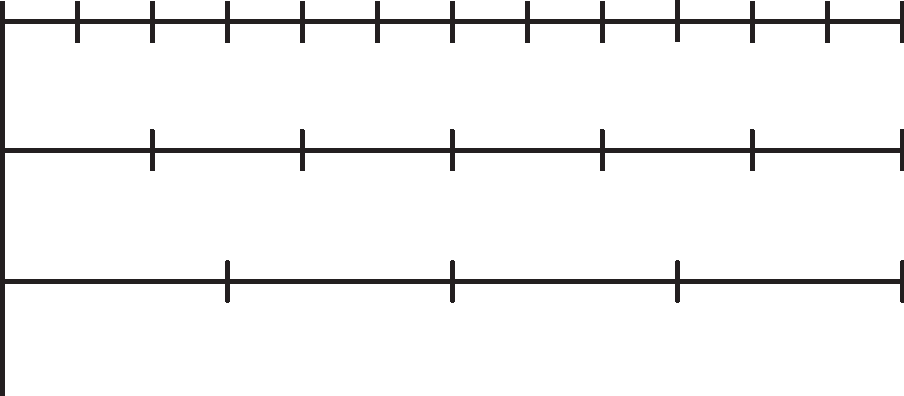
\includegraphics[width=0.7\textwidth]{gesamttex/edit_VIII,3/images/LH_37_01_001-002,003-008,025_d3a.pdf}
\end{minipage}
\hspace*{4mm}
\begin{minipage}[t]{0.5\textwidth}
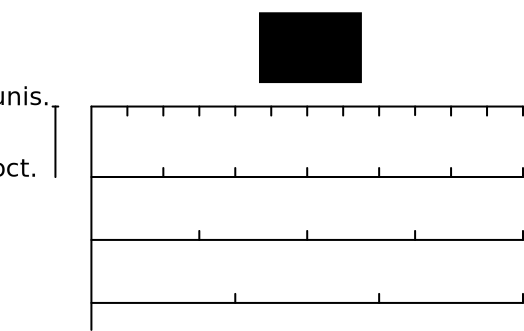
\includegraphics[width=0.91\textwidth]{gesamttex/edit_VIII,3/images/LH_37_01_001-002,003-008,025_d3b.pdf}
\end{minipage}
%\vspace{0.5em}
\newline
\noindent
\\
\hspace*{0.5mm} [\textit{Fig.~3a, gestr.; Lil (Bl.~7~v\textsuperscript{o}\!)}\label{LH_37_01_007v_f-3}]\hspace*{42mm} [\textit{Fig.~3b; L\textsuperscript{2}\! (Bl.~25~v\textsuperscript{o}\!)}]
%\vspace{1em}
\pend
%%%%%%%%%%%%%%%%%%%%%%%%%%%%%%%%%%%%%%%%%%%%%%%%%%
%
%  \vspace*{4.0em}%
%  \centerline{\hspace*{-70mm}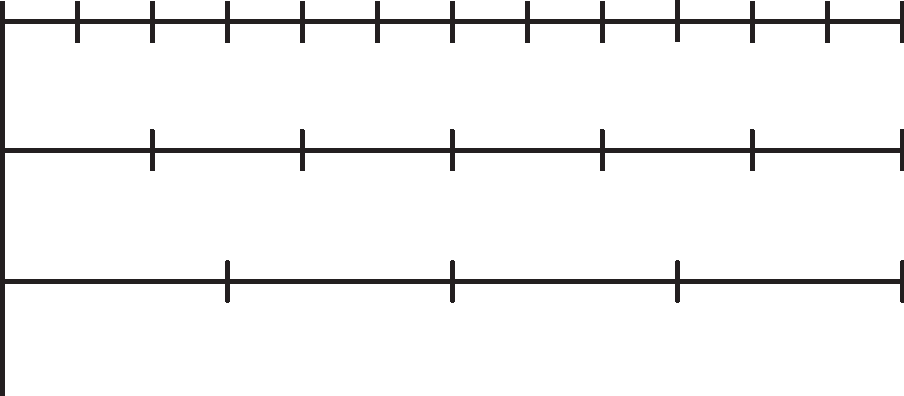
\includegraphics[width=0.34\textwidth]{gesamttex/edit_VIII,3/images/LH_37_01_001-002,003-008,025_d3a.pdf}}%\\
%  \vspace*{0.0em}
%  \centerline{\hspace*{-70mm}\lbrack\textit{Fig.~3a, gestr.; Lil (Bl.~7~v\textsuperscript{o}\!)}\rbrack}%
%  \label{LH_37_01_007v_f-3}%
%   \vspace*{1.5em}%
%  \newpage
%
%
%  \newpage
%  \pstart
%  \phantom{x}%
%%  \pend
%  \vspace*{-10.0em}% Rein provisorisch!
%  \centerline{\hspace*{60mm}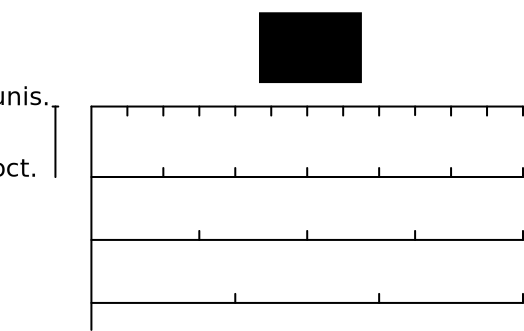
\includegraphics[width=0.42\textwidth]{gesamttex/edit_VIII,3/images/LH_37_01_001-002,003-008,025_d3b.pdf}}%\\
%  \vspace*{0.5em}
%  \centerline{\hspace*{60mm}\lbrack\textit{Fig.~3b; L\textsuperscript{2}\! (Bl.~25~v\textsuperscript{o}\!)}\rbrack}
%%  \vspace*{1.5em}%
  \newpage
  \count\Bfootins=900
\count\Afootins=900
\count\Cfootins=900
\pstart%
His\edlabel{LH_37_01_007v_ratiosuperius}\edlabel{LH_37_01_007v_pauloante_svdeatf-1}
ita
\edtext{positis vibratio aeris\protect\index{Sachverzeichnis}{vibratio aeris}
perveniens ad portionem aeris\protect\index{Sachverzeichnis}{portio aeris}
aliud}{%
\lemma{positis}\Bfootnote{\hspace{-0.5mm}%
\textit{(1)}~aer incidens in aliud
\textit{(2)}~vibratio aeris perveniens ad portionem \textbar~aeris \textit{erg.}~\textbar\ aliud%
~\textit{L\textsuperscript{1}}}}
%
corpus tensum\protect\index{Sachverzeichnis}{corpus tensum} attingentem,
exempli causa chordam novam\protect\index{Sachverzeichnis}{chorda nova}
\edtext{a prima chorda sonante\protect\index{Sachverzeichnis}{chorda sonans} non nimis remotam,
infligit illi ictum\protect\index{Sachverzeichnis}{ictus chordae} aliquem\lbrack,\rbrack\
unde vibrationes;
sed si illae non consentiant}{%
\lemma{a}\Bfootnote{\hspace{-0.5mm}%
\textit{(1)}~sonoro corpore distantem
\textit{(2)}~prima chorda \lbrack...\rbrack\ nimis remotam,
\textit{(a)}~imprimit illi quoque vibra
\textit{(b)}~infligit illi ictum aliquem
\textit{(aa)}~et inde
\textit{(bb)}~unde
\textit{(aaa)}~tremor. Sed i
\textit{(bbb)}~vibrationes, sed si illae
\textbar\ non \textit{erg.}~\textbar\ consentiant%
~\textit{L\textsuperscript{1}}%
\hspace{0.5mm}
a prima \lbrack...\rbrack\ non consentiant%
~\textit{l}}}
%
vibrationibus aeris\protect\index{Sachverzeichnis}{vibratio aeris}
aut chordae\protect\index{Sachverzeichnis}{vibratio chordae}
\edtext{prioris}{%
\lemma{prioris~,~\textit{L\textsuperscript{1}}}\Bfootnote{%
prioris~\textit{l}}}
%
tunc nova
\edtext{chorda\protect\index{Sachverzeichnis}{chorda nova}
vibrationem in se tota satis sensibilem\protect\index{Sachverzeichnis}{vibratio sensibilis} non accipit,}{%
\lemma{chorda}\Bfootnote{\hspace{-0.5mm}% 
\textit{(1)}~mox conquiescit
\textit{(2)}~vibrationem in \lbrack...\rbrack\ non accipit;%
~\textit{L\textsuperscript{1}}%
\hspace{0.5mm}
chorda vibrationem \lbrack...\rbrack\ non accipit,%
~\textit{l}}}
%
novae enim vibrationes\protect\index{Sachverzeichnis}{vibratio nova}
\edtext{\lbrack in ea\rbrack}{%
\lemma{in}\Bfootnote{\hspace{-0.5mm}%
ea \textit{erg.~L\textsuperscript{1}, fehlt~l, erg.~Hrsg.}}}
%
nascentes
\edtext{mox contrariis aeris vibrationibus\protect\index{Sachverzeichnis}{vibratio aeris} % \lbrack a\rbrack\ 
a quibus ortae sunt, rursus suffocantur,
sed}{%
\lemma{mox}\Bfootnote{\hspace{-0.5mm}%
\textit{(1)}~in
\textit{(2)}~a contrariis aeris vibrationibus
\textit{(a)}~iterum
\textit{(b)}~a quibus
\textit{(aa)}~natae
\textit{(bb)}~ortae sunt, rursus suffocantur. Sed%
~\textit{L\textsuperscript{1}}%
\hspace{0.5mm}
mox
\textbar~a \textit{fehlt}~%
\textbar\ contrariis aeris \lbrack...\rbrack\ rursus suffocantur, sed%
~\textit{l}}}
%
si chorda nova priori sit unisona,\protect\index{Sachverzeichnis}{chorda unisona}
seu vibrationes habeat isochronas\protect\index{Sachverzeichnis}{vibratio isochrona}
\edtext{\lbrack tunc eae\rbrack}{%
\lemma{tunc}\Bfootnote{\hspace{-0.5mm}%
\textbar~eae \textit{erg.}~\textbar%
~\textit{L\textsuperscript{1}, fehlt~l, erg. Hrsg.}}}
%
sequentibus aeris vibrationibus\protect\index{Sachverzeichnis}{vibratio aeris}
a chorda\protect\index{Sachverzeichnis}{chorda vibrans} priore venientibus\lbrack,\rbrack\
non tantum non destruuntur sed
\edtext{et}{%
\lemma{et}\Bfootnote{\hspace{-0.5mm}%
\textit{erg.~L\textsuperscript{1}}}}
%
potius augentur,\protect\index{Sachverzeichnis}{vibratio aucta}
novis semper
\edtext{ictibus\protect\index{Sachverzeichnis}{ictus novus}
inter se conspirantibus\protect\index{Sachverzeichnis}{ictus conspirans}
sive eodem tendentibus,\protect\index{Sachverzeichnis}{ictus tendens} inflictis;}{%
\lemma{ictibus}\Bfootnote{\hspace{-0.5mm}%
\textit{(1)}~inflictibus\lbrack\textit{!}\rbrack\
\textit{(2)}~inter se \lbrack...\rbrack\ tendentibus, inflictis;%
~\textit{L\textsuperscript{1}}}}
%
unde tandem sensibilis satis vibratio\protect\index{Sachverzeichnis}{vibratio sensibilis}
imo sonus\protect\index{Sachverzeichnis}{sonus sensibilis}
chordae novae\protect\index{Sachverzeichnis}{chorda nova}
priori unisonae\protect\index{Sachverzeichnis}{chorda unisona}
\edlabel{KZeitz53}\edtext{}{{\xxref{KZeitz53}{KZeitz54}}%
{%
\lemma{nasci}\Bfootnote{\hspace{-0.5mm}%
\textit{(1)}~potest
\textit{(2)}~solet \textbar~ut pila \lbrack...\rbrack\ celeritatem acquirit \textit{erg.}~%
\textbar~. Ubi tamen duo notanda sunt,
\textbar~primum \textit{erg.}~%
\textbar\ etiam%
~\textit{L\textsuperscript{1}}%
\hspace{0.5mm}
nasci solet, ut \lbrack...\rbrack\ celeritatem acquirit.
\textit{(1)}~Ubi tamen \textso{duo} notanda sunt, \textso{primum}~\textit{l}
\textit{(2)}~Et tale \lbrack...\rbrack\ Cl. Schel\-hammerus.
\textit{(a)}~Ita tamen notandum
\textit{(b)}~Tria tamen \lbrack...\rbrack\ duplicis octavae
\textit{(aa)}~et
\textit{(bb)}~,
\textit{(cc)}~et quintae \textbar~et $\langle$quartae$\rangle$ \textit{gestr.}~\textbar~,
\textit{(aaa)}~quia
\textit{(bbb)}~in quibus \lbrack...\rbrack\ aut tertii
\textit{(aaaa)}~aut sexti aut duodecimi % \textit{gestr.}~%
\textit{(bbbb)}~quique ictus conveniunt. \textso{Secundo,}~\textit{Lil}
etiam%
~\textit{l}}}}%
nasci solet,
ut pila in planitie decurrens\protect\index{Sachverzeichnis}{pila decurrens}
repetitis ictibus\protect\index{Sachverzeichnis}{ictus repetitus} eorum
quos currendo praeterit magnam satis celeritatem\protect\index{Sachverzeichnis}{celeritas acquisita} acquirit.
%
\edlabel{LH_37_01_007v_w1}Et tale quid,
licet ob non satis cognitam potentiae Elasticae\protect\index{Sachverzeichnis}{potentia elastica} naturam,\protect\index{Sachverzeichnis}{natura}
\edtext{obscure et per nebulam vidit olim Fracastorius,\protect\index{Namensregister}{\textso{Fracastoro} (Fracastorius), Girolamo 1478\textendash1553}}{%
\lemma{obscure \lbrack...\rbrack\ Fracastorius}\Cfootnote{%
Siehe \textsc{G.~Fracastoro}, \textit{De sympathia}, cap.~4 % et antipathia, 
(Venedig 1546, S.~3~r\textsuperscript{o}/v\textsuperscript{o};
\textit{Opera}~I, Lyon 1591, S.~9\,f.).\cite{01215}}}
cujus locum mihi
\edtext{indicavit}{%
\lemma{indicavit}\Cfootnote{%
Siehe \textsc{% G.~C. 
Schelhammer}, Brief an Leibniz vom 13. (23.) April 1681 (\textit{LSB} III,~3 N.~206, S.~398.3\textendash5).\cite{01200}}}
et postea eleganti atque erudito
\edtext{libro de organo auditus inseruit}{%
\lemma{libro \lbrack...\rbrack\ inseruit}\Cfootnote{%
Siehe \textsc{% G.~C. 
Schelhammer}, \textit{De auditu}, % Leiden 1684, 
S.~125\,f.\cite{01204}
Leibniz hat die Passage exzerpiert (N.~12\textsubscript{4}, S.~\refpassage{LH_37_01_014_a1}{LH_37_01_014_a2}).}}
Cl. Schelhammerus.\protect\index{Namensregister}{\textso{Schelhammer} (Schelhammerus), Günther Christoph 1649\textendash1716}%
\edlabel{LH_37_01_007v_w2}
Tria tamen adhuc notanda.%
\textso{ Primo }%
\edlabel{LH_37_01_007v-koinzidenztheorie-1}%
\edtext{quod de unisono\protect\index{Sachverzeichnis}{unisonus} diximus
aliquo modo porrigi ad intervalla $\langle$co$\rangle$ncinniora,\protect\index{Sachverzeichnis}{intervallum concinnum}
ut octavae,\protect\index{Sachverzeichnis}{octava}
duplicis octavae\protect\index{Sachverzeichnis}{octava duplex}
et quintae,\protect\index{Sachverzeichnis}{quinta}
in quibus non quidem omnes
tamen $\langle$a$\rangle$lterni aut tertii quique ictus\protect\index{Sachverzeichnis}{ictus alternus} conveniunt.%
\edlabel{LH_37_01_007v-koinzidenztheorie-2}%
}{%
\lemma{quod \lbrack...\rbrack\ conveniunt}\Cfootnote{%
Den hier ausgeführten Grundgedanken der Koinzidenztheorie kannte Leibniz etwa aus
\textsc{Galilei}, \textit{Discorsi}, S.~103\textendash107\cite{00050}
(\textit{GO} VIII, S.~146.20\textendash150.14).\cite{00048}}}%
\textso{ Secundo,}\edlabel{LH_37_01_007v_moxexperimentum-1} etiam\edlabel{KZeitz54}
%
chordam non unisonam ex toto,\protect\index{Sachverzeichnis}{chorda unisona pro parte}
tamen intelligi posse unisonam pro
\edtext{parte;}{%
\lemma{parte~,~\textit{L\textsuperscript{1}}}\Bfootnote{%
parte~;~\textit{l}}}
%
\edtext{unde}{%
\lemma{unde}\Bfootnote{\hspace{-0.5mm}%
\textit{(1)}~notatum est
\textit{(2)}~observatum audio a viris
\textit{(a)}~diligentibus
\textit{(b)}~ingeniosis%
~\textit{L\textsuperscript{1}}}}
\edtext{observatum audio a viris\protect\index{Sachverzeichnis}{vir} ingeniosis}{%
\lemma{observatum \lbrack...\rbrack\ ingeniosis}\Cfootnote{%
Vermutlich Anspielung auf
\cite{01285}J.~\textsc{Wallis}, \glqq Letter concerning a new Musical Dis\-co\-very\grqq, \textit{PT} XII, Nr.~134 (1677), S.~839\textendash842.
Andeutungen auf das Phänomen der Obertöne finden sich auch in
\cite{01286}R.~\textsc{Des\-cartes}, Brief an M.~Mersenne vom 22.~Juli 1633 (\cite{00209}\textit{DL} II, S.~348\,f.;
\cite{00120}\textit{DO} I, S.~267.7\textendash268.6).}}%
\edlabel{KZeitz55}\edtext{}{{\xxref{KZeitz55}{KZeitz56}}%
{%
\lemma{chordam $TZ$ \lbrack...\rbrack\ ipsi $RS$}\Cfootnote{%
Siehe \lbrack\textit{Fig.~4d}\rbrack, S.~\pageref{LH_37_01_008r_f-4}.
In \textit{L\textsuperscript{1}} beziehen sich die gestrichenen Varianten auf das ebenso gestrichene Diagramm \lbrack\textit{Fig.~4a}\rbrack, S.~\pageref{LH_37_01_002v_a1.1}.}}}
chordam%
\edtext{ $TZ$ duplo}{%
\lemma{chordam}\Bfootnote{\hspace{-0.5mm}%
\textit{(1)}~$CE$
\textit{(2)}~$TZ$%
~\textit{L\textsuperscript{1}}}}
%
\lbrack8~r\textsuperscript{o}\rbrack\ %%%% Blatt 8r
%
longiorem
\edtext{altera $RS$ sed}{%
\lemma{altera}\Bfootnote{\hspace{-0.5mm}%
\hspace{-0.5mm}\textbar~%
\textit{(1)}~$AB$
\textit{(2)}~$RS$
\textit{erg.}~\textbar\ sed%
~\textit{L\textsuperscript{1}}}}
%
alias aeque
tensam\protect\index{Sachverzeichnis}{chorda aeque tensa}
\edtext{crassamque,\protect\index{Sachverzeichnis}{chorda aeque crassa}
non totam quidem attamen duabus suis medietatibus
$TV,$ $VZ$ singulatim,
priori $RS$ nonnihil
(\phantom)\hspace{-1.2mm}%
quod pennulis\protect\index{Sachverzeichnis}{pennula adhaerens} in locis \textit{X},\,\textit{X} adhaerentibus apparuit
\lbrack praesertim si chorda\protect\index{Sachverzeichnis}{chorda pulsata} $RS$
plectro\protect\index{Sachverzeichnis}{plectrum} moderate pulsetur\rbrack%
\phantom(\hspace{-1.2mm})
contremuisse,}{%
\lemma{crassamque}\Bfootnote{\hspace{-0.5mm}%
\textit{(1)}~in duas partes fuisse divisam ut
\textit{(2)}~non totam quidem attamen duabus \textbar~suis \textit{erg.}~\textbar\ medietatibus
\textit{(a)}~$CD$ \textbar~et \textit{erg.}~\textbar\ $DE$
\textit{(b)}~$TV,$ $VZ$ \textbar~singulatim \textit{erg.}~%
\textbar\ priori
\textit{(aa)}~$AB$
\textit{(bb)}~$RS$ nonnihil (\phantom)\hspace*{-1.2mm}quod
\textit{(aaa)}~plumae adhaerentes\protect\index{Sachverzeichnis}{pluma}
\textit{(bbb)}~plumis adhaerentibus \textbar~in $P,$\,$P$ \textit{erg.}~\textbar\ appa\-ruit
\textit{(ccc)}~pennulis in \lbrack...\rbrack\ adhaerentibus apparuit
\textbar~praesertim si chorda $AB$ plectro moderate pulsetur \textit{erg.}~%
\textbar~\phantom(\hspace{-1.2mm}) contremuisse,%
~\textit{L\textsuperscript{1}}%
\hspace{0.5mm}
crassamque~, non % totam quidem attamen duabus suis 
\lbrack...\rbrack\ medietatibus $TV,$ $VZ$
\textbar~et \textit{gestr.~Lil}~%
\textbar\ singulatim, priori $RS$
\lbrack...\rbrack\ adhaerentibus apparuit
\textbar~praesertim si chorda % \textbar~
$AB$ % \textit{ändert Hrsg.}~% \textbar\ 
plectro moderate pulsetur \textit{erg. Hrsg. nach~L\textsuperscript{1}, ändert Hrsg.}~%
\textbar~\phantom(\hspace{-1.2mm})
contremuisse,%
~\textit{l}}}
%
nam revera
\edtext{singulae partes $TV,$ $VZ$ ipsi $RS$}{%
\lemma{singulae}\Bfootnote{\hspace{-0.5mm}%
\textit{(1)}~partes
\textit{(2)}~partes
\textit{(a)}~$CD,$ $DE$
\textit{(b)}~$TV,$ $VZ$ ipsi
\textit{(aa)}~$AB$
\textit{(bb)}~$RS$%
~\textit{L\textsuperscript{1}}}}\edlabel{KZeitz56}
%
sunt
\edtext{unisonae,\protect\index{Sachverzeichnis}{pars unisona}}{%
\lemma{unisonae~;~\textit{L\textsuperscript{1}}}\Bfootnote{%
unisonae~,%
~\textit{l}}}
%
et putem determinari quoque posse,
quid in aliis chordarum duarum proportionibus sit futurum\lbrack;\rbrack\
\edlabel{KZeitz57}\edtext{}{{\xxref{KZeitz57}{KZeitz58}}%
{%
\lemma{quae \lbrack...\rbrack\ servetur}\Cfootnote{%
In \textit{L\textsuperscript{1}} auf Bl.~1~r\textsuperscript{o} verfasst.}}}%
quae res
\edtext{iterum nostram}{%
\lemma{iterum}\Bfootnote{\hspace{-0.5mm}%
\textit{(1)}~nostrum
\textit{(2)}~nostram%
~\textit{L\textsuperscript{1}}}}
%
explicationem\protect\index{Sachverzeichnis}{explicatio} egregie illustrat,
nam ut hic in chorda\protect\index{Sachverzeichnis}{chorda pulsata} percipimus,
ita in aere\protect\index{Sachverzeichnis}{pars aeris}
\edtext{colligimus,}{%
\lemma{collegimus~\textit{L\textsuperscript{1}}}\Bfootnote{%
colligimus~,%
~\textit{l}}}
%
\edtext{partes sponte naturae\protect\index{Sachverzeichnis}{sponte naturae} assignari}{%
\lemma{partes}\Bfootnote{\hspace{-0.5mm}%
\textit{(1)}~assignari
\textit{(2)}~sponte naturae assignari%
~\textit{L\textsuperscript{1}}}}
%
\edtext{tales,}{%
\lemma{tales~\textit{L\textsuperscript{1}}}\Bfootnote{%
tales~,%
~\textit{l}}}
%
ut vibrationum isochronismus\protect\index{Sachverzeichnis}{isochronismus vibrationis} servetur.%
\edlabel{LH_37_01_008r_moxexperimentum-2}\edlabel{LH_37_01_008r_pauloante_svdeatf-2}\edlabel{KZeitz58}
% % Textabschnitt
% \pend%
% \newpage%
% \vspace*{0.5em}%
%
% \pstart%
% \noindent%
%
% % % % <ins-1> <<<<<<<<<<<<<<<<<<<<<<<<<<<<<<<<<<<<<<<<<<<<<<<<<<<<<<<<<<<<<<<<<<<<<<<<<<<<<<<<<<<<<<<<<<
% \lbrack\textit{Nachfolgender, im Konzept L\textsuperscript{1}\! fehlender Textabschnitt (bis zu S.~\refpassage{LH_37_01_008r_a1}{LH_37_01_008r_a2}) wurde in der Reinschrift l am Rand von Bl.~8~r\textsuperscript{o}\! ergänzt (Lil):}\rbrack\
% \pend%
%
% \pstart%
% \noindent%
\edtext{}{%
{\xxref{LH_37_01_008r_a11}{LH_37_01_008r_a2}}%
{\lemma{Quibus consentiunt \lbrack...\rbrack\ in \textlangle\textit{V.}\textrangle}\Bfootnote{%
\textit{fehlt~L\textsuperscript{1}, erg.~Lil}}}%
{\lemma{Quibus \lbrack...\rbrack\ in \textlangle\textit{V}\textrangle}\Cfootnote{% consentiunt
Der in \textit{L\textsuperscript{1}} fehlende Textabschnitt ist in \textit{l} am Rand von Bl.~8~r\textsuperscript{o}\! ergänzt (\textit{Lil}).}}}%
\edlabel{LH_37_01_008r_a11}Quibus consentiunt egregie,
\edtext{quae habet Chalesius\protect\index{Namensregister}{\textso{Dechales} (Chalesius), Claude François Milliet 1621\textendash1678} in \textit{Musica},}{%
\lemma{quae \lbrack...\rbrack\ \textit{Musica}}\Cfootnote{% 
Siehe \textsc{Dechales}, \textit{Cursus}, tract. XXII, prop.~16 (Bd.~III, S.~24a\textendash b).\cite{00124}}} %  C.\,F.\,M., seu mundus mathematicus, Lyon 1674, 
ad explicandos \edtext{Tubae\protect\index{Sachverzeichnis}{saltus tubae} et fistularum\protect\index{Sachverzeichnis}{saltus fistulae} saltus
a Mersenno\protect\index{Namensregister}{\textso{Mersenne}, Marin 1588\textendash1648} propositos}{%
\lemma{Tubae \lbrack...\rbrack\ propositos}\Cfootnote{%
Siehe \textsc{Mersenne}, \textit{Harmonie universelle}, livre V des instrumens, prop. 12 (Bd.~II, S.~D~249\textendash251).\cite{01205}}}%
\lbrack:\rbrack\
dum enim vehementius inspiratur \edtext{\lbrack tubae\rbrack,}{%
\lemma{tuba,\protect\index{Sachverzeichnis}{tuba}}\Bfootnote{%
\textit{Lil~ändert Hrsg.}}}
cogitur aer ad celeriorem motum,\protect\index{Sachverzeichnis}{motus aeris}
cumque in tota tuba vibratio\protect\index{Sachverzeichnis}{vibratio tubae}
sit per modum unius chordae,
chorda autem tantae longitudinis\protect\index{Sachverzeichnis}{longitudo chordae}
tantum motum\protect\index{Sachverzeichnis}{motus chordae} facile praestare non possit,
dividitur tota haec quasi chorda per medium et bifariam,\protect\index{Sachverzeichnis}{chorda divisa}
ut ita dividatur in partes consonas\protect\index{Sachverzeichnis}{pars consona}
(\phantom)\hspace{-1.2mm}%
ne vibrationes\protect\index{Sachverzeichnis}{vibratio chordae} se mutuo perturbent%
\phantom(\hspace{-1.2mm}).
\edtext{\textit{Atque hoc se} quoque
\textit{expertum refert Galilaeus,\protect\index{Namensregister}{\textso{Galilei} (Galilaeus, Galileus), Galileo 1564\textendash1642}
cum enim laminam aeream\protect\index{Sachverzeichnis}{lamina aerea}
aut ferream\protect\index{Sachverzeichnis}{lamina ferrea} aliquando ita tereret,
ut ejus etiam vibrationes\protect\index{Sachverzeichnis}{vibratio laminae} animadverteret,
quotiescunque motus ejus erat concitatior,
non tota lamina per modum unius vibrabatur,
sed dividebatur vibratio\protect\index{Sachverzeichnis}{vibratio laminae} in duas,
et tonus\protect\index{Sachverzeichnis}{tonus} ascendebat per octavam.\protect\index{Sachverzeichnis}{octava}
Ita dum scyphi aqua pleni\protect\index{Sachverzeichnis}{scyphus aqua plenus}
labra digito\protect\index{Sachverzeichnis}{digitus} teruntur
si vehementior sit motus ascendit sonus\protect\index{Sachverzeichnis}{ascensus soni} ad octavam\protect\index{Sachverzeichnis}{octava}}}{%
\lemma{\textit{Atque} \lbrack...\rbrack\ \textit{octavam}}\Cfootnote{%
\textsc{Dechales}, \textit{Cursus}, tract. XXII, prop.~16 %  seu mundus mathematicus, Lyon 1674, 
(Bd.~III, S.~25a).\cite{00124}
% Das Referat ist etwas ungenau;
Vgl. \textsc{Galilei}, \textit{Discorsi}, S.~98\textendash102 (\textit{GO}~VIII, S.~141\textendash145).\cite{00050}\cite{00048}}}% Leiden 1638, 
\edtext{.
\edlabel{LH_37_01_008r_rv1}%
Hinc}{%
\lemma{\textit{octavam.}}\Bfootnote{%
\textit{(1)}~Haec
\textit{(a)}~Ca
\textit{(b)}~Chalesius\protect\index{Namensregister}{\textso{Dechales} (Chalesius), Claude François Milliet 1621\textendash1678}
\textit{(2)}~Hinc%
~\textit{Lil}}}
etiam ut obiter dicam, veram, ni fallor,
\edtext{rationem\protect\index{Sachverzeichnis}{ratio} inveni,}{%
\lemma{rationem inveni}\Cfootnote{%
Siehe aber bereits \cite{01285}\textsc{Wallis}, \glqq Letter concerning a new Musical Discovery\grqq, S.~842.}}%
%
\textso{ cur is }%
\edtext{\textso{qui vitrum}\protect\index{Sachverzeichnis}{vitrum}\textso{ soni}}{%
\lemma{\textso{qui}}\Bfootnote{%
\textit{(1)}~\textso{soni}
\textit{(2)}~\textso{vitrum soni}%
~\textit{Lil}}}%
\textso{ vehementia}\protect\index{Sachverzeichnis}{vehementia soni}%
\textso{ rumpere conatur }%
\edtext{\textso{ascendat ad octavam}\protect\index{Sachverzeichnis}{octava}\protect\index{Sachverzeichnis}{ascensus soni}}{%
\lemma{\textso{ascendat ad octavam}}\Cfootnote{%
Siehe \cite{01207}\textsc{Morhof}, \textit{De scypho vitreo}, S.~16\,f.}}% cap.~1 
%
\textso{ }ejus soni
quem in vitro pulsatione\protect\index{Sachverzeichnis}{pulsatio} explorato
\edtext{comperit\lbrack,\rbrack\
nam ita et vibrationes\protect\index{Sachverzeichnis}{vibratio vitri} fient tanto velociores,
et cum totum vitrum,\protect\index{Sachverzeichnis}{vitrum}
nec consentienter vibretur,\protect\index{Sachverzeichnis}{vibratio consentiens}
nec tam vehementem agitationem\protect\index{Sachverzeichnis}{agitatio} facile recipiat,
potius dividetur bifariam, nam quaelibet pars}{%
\lemma{comperit}\Bfootnote{%
\textit{(1)}~cum enim
\textit{(2)}~nam ita et vibrationes
\textit{(a)}~fiunt
\textit{(b)}~fient tanto \lbrack...\rbrack\ totum vitrum,
\textit{(aa)}~licet sono quem is edit consonum, tam vehementem agitationem non
\textit{(bb)}~nec consentienter \lbrack...\rbrack\ recipiat, potius
\textit{(aaa)}~dividitur
\textit{(bbb)}~dividetur bifariam,
\textit{(aaaa)}~ut quaelibet pars si
\textit{(bbbb)}~nam quaelibet pars%
~\textit{Lil}}}
%
facilius agitatur, et
(\phantom)\hspace{-1.2mm}%
cum dimidium ad octavam\protect\index{Sachverzeichnis}{octava}
ascendat\protect\index{Sachverzeichnis}{ascensus soni} respectu totius%
\phantom(\hspace{-1.2mm})
eo ipso cum eo qui sonum edit, perfecte consonat, non minus quam una pars alteri;
vibrationesque\protect\index{Sachverzeichnis}{vibratio vitri} non sese mutuo confundunt,
sed juvant, atque magis magisque intendunt.
Cum vero sonus et valde sit vehemens,\protect\index{Sachverzeichnis}{sonus vehemens}
et satis diu\protect\index{Sachverzeichnis}{sonus continuatus}
\edtext{continuatus,
(\phantom)\hspace{-1.2mm}%
quae duo ad rumpenda sono vitra\protect\index{Sachverzeichnis}{vitrum} requiruntur%
\phantom(\hspace{-1.2mm})
continuatis semper novis impulsibus,\protect\index{Sachverzeichnis}{impulsus continuatus}
motum continuo acceleratum\protect\index{Sachverzeichnis}{motus acceleratus}}{%
\lemma{continuatus,}\Bfootnote{%
\textit{(1)}~continuatis semper novis impulsibus motum continue acceleratum
\textit{(2)}~(\phantom)\hspace{-1.2mm}quae duo \lbrack...\rbrack\ continuo acceleratum%
~\textit{Lil}}}
tantumque denique impetum\protect\index{Sachverzeichnis}{impetus conceptus}
concipiunt partes duae vitri\protect\index{Sachverzeichnis}{vitrum} separatim
(\phantom)\hspace{-1.2mm}%
licet consentienter%
\phantom(\hspace{-1.2mm})
vibrantes,
\edtext{ut tandem}{%
\lemma{ut}\Bfootnote{%
\textit{(1)}~denique
\textit{(2)}~tandem%
~\textit{Lil}}}
vis\protect\index{Sachverzeichnis}{vis vibrandi}
\edtext{vibrandi et conatus excurrendi,\protect\index{Sachverzeichnis}{conatus excurrendi}
major fiat vitri firmitate;\protect\index{Sachverzeichnis}{firmitas vitri}}{%
\lemma{vibrandi}\Bfootnote{%
\textit{(1)}~major fiat vitri fi
\textit{(2)}~et conatus \lbrack...\rbrack\ vitri firmitate;%
~\textit{Lil}}}
quo facto ruptura\protect\index{Sachverzeichnis}{ruptura vitri}
\edtext{sequetur.
Si enim vitrum\protect\index{Sachverzeichnis}{vitrum} concipiamus
per modum lineae seu chordae\protect\index{Sachverzeichnis}{chorda vibrans} $TZ,$}{%
\lemma{sequetur.}\Bfootnote{%
\textit{(1)}~Si enim vitrum concipiamus per modum lineae $TZ$
\textit{(2)}~Si enim \lbrack...\rbrack\ chordae $TZ,$%
~\textit{Lil}}}
divisum in duas partes $TV,$
\edtext{\lbrack $VZ$\rbrack ,}{%
\lemma{$XZ$}\Bfootnote{\textit{Lil~ändert Hrsg.}}}
separatim vibrantes,\protect\index{Sachverzeichnis}{pars vibrans}
in $TPV,$ $VQZ$ eodem tempore;\protect\index{Sachverzeichnis}{tempus vibrationis}
et rursus eodem tempore transferendas in $TNV,$
\edtext{$VOZ$\lbrack,\rbrack\ patet}{%
\lemma{$VOZ$}\Bfootnote{%
\textbar~ubi \textit{gestr.}~\textbar\ patet%
~\textit{Lil}}}
punctum $V$ quod eas connectit,
atque earum libertatem\protect\index{Sachverzeichnis}{libertas} coercet,
magnam vim\protect\index{Sachverzeichnis}{vis magna} sentire debere
inter tot flexuum commutationes,\protect\index{Sachverzeichnis}{commutatio flexus}
et conceptos a reliquis partibus longius excurrere conantibus
\edtext{impetus\protect\index{Sachverzeichnis}{impetus conceptus} quibus}{%
\lemma{impetus}\Bfootnote{%
\textit{(1)}~talibus
\textit{(2)}~quibus%
~\textit{Lil}}}
ipsum, solum immotum manens, resistit.
Unde firmitas\protect\index{Sachverzeichnis}{firmitas vitri} ejus,
\edtext{vi vibrationum\protect\index{Sachverzeichnis}{vis vibrationis} atque celerrimorum excursuum nimis}{%
\lemma{vi}\Bfootnote{%
\textit{(1)}~nimis
\textit{(2)}~vibrationum atque celerrimorum excursuum nimis%
~\textit{Lil}}}
aucta et distrahente,\protect\index{Sachverzeichnis}{vis distrahens} tandem
\edlabel{KZeitz59}\edtext{}{{\xxref{KZeitz59}{KZeitz60}}%
{%
\lemma{superabitur}\Bfootnote{%
\textit{(1)}~quemadmodum et baculus saepe in diversa flexus, tandem in medio ita ruet
\textit{(2)}~. Idem
\textit{(3)}~. Idem est
\textit{(4)}~. Idem est \lbrack...\rbrack\ ita $\langle$ut$\rangle$
\textit{(a)}~$TZ$
\textit{(b)}~$TVZ$ translatum \lbrack...\rbrack\ modo flexi\phantom(\hspace{-1.2mm})%
~\textit{Lil}}}}%
superabitur.
Idem est si utrum non ex statu $TPVQZ$\protect\index{Sachverzeichnis}{status} in statum $TNVOZ,$
sed ex statu $TPVOZ$ in statum $TNVQZ$\protect\index{Sachverzeichnis}{status} transferatur.
Sed multo adhuc magis locum habebit
si \edlabel{LH_37_01_008r_b1}%
\edtext{}{\xxref{LH_37_01_008r_b1}{LH_37_01_008r_b2}{%
\lemma{pun$\langle$cta$\rangle$ \lbrack...\rbrack\ in $\langle V.\rangle$}\Cfootnote{%
Die in \textit{l} befindlichen Textverluste sind unter Berücksichtigung von \textit{E}, S.~25 ergänzt.}}}%
pun$\langle$cta$\rangle$ % \edtext{}{\lemma{pun$\langle$cta$\rangle$}\Cfootnote{Nach \textit{E}, S.~25 ergänzt.}}
$T,$ $Z$ a connexione duarum partium vitri\protect\index{Sachverzeichnis}{vitrum} maxime remota,
non immota sed libere vibrantia, ut revera sunt, concipiamus,
ita $\langle$ut$\rangle$ % \edtext{}{\lemma{$\langle$ut$\rangle$}\Cfootnote{Nach \textit{E}, S.~25 ergänzt.}}
%
$TVZ$ translatum in $WVY$ redeat in \textit{3V4},
ita enim facile
(\phantom)\hspace{-1.2mm}%
ad baculi\protect\index{Sachverzeichnis}{baculus flexus} instar hoc modo flexi%
\phantom(\hspace{-1.2mm})\edlabel{KZeitz60}
frangetur vitrum\protect\index{Sachverzeichnis}{vitrum fractum}
\edlabel{LH_37_01_008r_sfkjlerzl-1}in
%************+
$\langle V.\rangle$\edlabel{LH_37_01_008r_b2}% \edtext{}{\lemma{$\langle V.\rangle$}\Cfootnote{Nach \textit{E}, S.~25 ergänzt.}}%
\edtext{}{%
{\xxref{LH_37_01_008r_sfkjlerzl-1}{LH_37_01_008r_sfkjlerzl-2}}%
{\lemma{in}\Bfootnote{\hspace{-0.5mm}%
$\langle V.\rangle$~\textit{fehlt}
Alterum
\textit{L\textsuperscript{1}}%
\hspace{0.5mm}
in $\langle V.\rangle$~\textit{Lil}
\textit{(1)}~\textso{Alterum}~\textit{l}
\textit{(2)}~\textso{Tertium}%
~\textit{Lil}}}}%
\edlabel{LH_37_01_008r_a1}\edlabel{LH_37_01_008r_a2}\edlabel{LH_37_01_008r_rv2}
% \lbrack\textit{Hier endet der in l am Rand von Bl.~8~r\textsuperscript{o} ergänzte Textabschnitt (Lil).}\rbrack
% % % % </ins-1> <<<<<<<<<<<<<<<<<<<<<<<<<<<<<<<<<<<<<<<<<<<<<<<<<<<<<<<<<<<<<<<<<<<<<<<<<<<<<<<<<<<<<<<<<<
%
% \pend%
% \newpage%
% \vspace*{0.5em}%
%
% \pstart%
% \noindent%
%
\textso{Tertium}\edlabel{LH_37_01_008r_sfkjlerzl-2}%
\textso{ }quod hic
\edtext{notandum videbatur,
hoc erat quod chorda chordam unisonam\protect\index{Sachverzeichnis}{chorda unisona}
melius imitatur si in eadem sint tabula,\protect\index{Sachverzeichnis}{tabula lignea}
lignum\protect\index{Sachverzeichnis}{lignum} enim
velut corpus solidius\protect\index{Sachverzeichnis}{corpus solidum}}{%
\lemma{notandum~,}\Bfootnote{\hspace{-0.5mm}%
hoc erat, quod
\textit{(1)}~duae chordae unisonae
\textit{(2)}~chorda chordam unisonam
\textit{(a)}~facilius
\textit{(b)}~clarius
\textit{(c)}~expressius imitatur,
\textit{(aa)}~si interventu ligni quam aeris vel alterius corporis solidioris
\textit{(bb)}~si in % eadem sint tabula, lignum 
\lbrack...\rbrack\ enim, velut corpus solidius,%
~\textit{L\textsuperscript{1}}%
\hspace{0.5mm}
notandum
\textbar~videbatur \textit{erg.~Lil}~%
\textbar~, hoc erat \lbrack...\rbrack\
 chordam unisonam
\textbar~melius \textit{erg.~Lil}~%
\textbar\ imitatur si \lbrack...\rbrack\ corpus solidius%
~\textit{l}}}
%
sonum\protect\index{Sachverzeichnis}{sonus propagatus} fortius
\edtext{propagat, et hanc}{%
{\lemma{propagat~.}\Bfootnote{\hspace{-0.5mm}%
Et hanc%
~\textit{L\textsuperscript{1}}%
\hspace{0.5mm}
propagat~,
\protect\index{Sachverzeichnis}{effectus}\protect\index{Sachverzeichnis}{tuba stentorea}%
\textbar~quod utile est ad explicandum effectum \textso{tubae stentoreae} de quo alias \textit{erg.~u. gestr.~Lil}~%
\textbar\ et hanc%
~\textit{l}}}%
{\lemma{propagat, et hanc}\Cfootnote{{%
Siehe über die im gestr. Text erwähnte \textit{tuba stentorea} die Auf\-zeich\-nung N.~2.}}}}
%
in rem notari potest
\edtext{}{{\xxref{LH_37_01_008r_c1}{LH_37_01_008r_c2}}{%
\lemma{experimentum \lbrack...\rbrack\ amota}\Cfootnote{%
Anspie\-lung auf einen im \textit{JS}, 16. u. 23. März 1665 (Pariser
 Ausgabe: S.~148\textendash150; 161)
anonym ver\-öf\-fent\-lichten Bericht über das Phänomen der \glqq Sympathie\grqq\ unter Uhrwerken,
dessen Verfasser eigentlich Christiaan Huygens ist; vgl. \textit{HO}~V, Nr.~1335, S.~243\,f.\cite{01201}}}}%
\edtext{\edlabel{LH_37_01_008r_c1}experimentum\protect\index{Sachverzeichnis}{experimentum horologiorum} in diario}{%
\lemma{experimentum}\Bfootnote{\hspace{-0.5mm}%
in diario%
~\textit{L\textsuperscript{1}}%
\hspace{0.5mm}
experimentum
\textbar~in \textit{erg.~Lil}~%
\textbar\ diario%
~\textit{l}}}
%
eruditorum Gallico aliquando
\edtext{relatum}{%
\lemma{relatum~,~\textit{L\textsuperscript{1}}}\Bfootnote{%
relatum%
~\textit{l}}}
%
de duobus horologiis\protect\index{Sachverzeichnis}{horologium}
\edtext{ab eodem ligneo sustentaculo\protect\index{Sachverzeichnis}{sustentaculum} suspensis\lbrack,\rbrack}{%
\lemma{ab}\Bfootnote{\hspace{-0.5mm}%
\textit{(1)}~eadem
\textit{(2)}~eodem
\textit{(a)}~ligno suspensis
\textit{(b)}~ligneo sustentaculo suspensis,%
~\textit{L\textsuperscript{1}}%
\hspace{0.5mm}
ab eodem ligneo sustentaculo suspensis%
~\textit{l}}}
%
quorum vibrationes\protect\index{Sachverzeichnis}{vibratio horologii}
perfecte
\edtext{congruebant\protect\index{Sachverzeichnis}{vibratio congruens} aut}{%
\lemma{congruebant}\Bfootnote{\hspace{-0.5mm}%
\textit{(1)}~vel
\textit{(2)}~aut%
~\textit{L\textsuperscript{1}}}}
%
ex composito turbatae ad concordiam\protect\index{Sachverzeichnis}{concordia vibrationum}
\edtext{redibant\lbrack;\rbrack\
quod}{%
\lemma{redibant~;}\Bfootnote{\hspace{-0.5mm}%
\textit{(1)}~donec c
\textit{(2)}~quod%
~\textit{L\textsuperscript{1}}%
\hspace{0.5mm}
redibant quod%
~\textit{l}}}
%
sola aeris connexio\protect\index{Sachverzeichnis}{connexio aeris}
non
\edtext{effecisset\lbrack,\rbrack\
cessavit enim consensus,\protect\index{Sachverzeichnis}{consensus vibrationum}
ubi a communi sustentaculo\protect\index{Sachverzeichnis}{sustentaculum}
sunt amota:\edlabel{LH_37_01_008r_c2}
patet}{%
\lemma{effecisset~.}\Bfootnote{\hspace{-0.5mm}% 
Patet%
~\textit{L\textsuperscript{1}}%
\hspace{0.5mm}
effecisset
\textbar~cessavit enim \lbrack...\rbrack\ sunt amota: \textit{erg.~Lil}~%
\textbar\ patet%
~\textit{l}}}
%
autem ex his
quomodo chorda\protect\index{Sachverzeichnis}{chorda unisona pro parte} quaelibet
ipsumque adeo
\edtext{lignum\protect\index{Sachverzeichnis}{lignum}}{%
\lemma{lignum~,~\textit{L\textsuperscript{1}}}\Bfootnote{%
lignum%
~\textit{l}}}
%
pro diversis suis partibus cuilibet alteri corpori unisonum intelligi
\edtext{possit,
unum tamen corpus alio aptius et aptissime omnium aer\protect\index{Sachverzeichnis}{aer unisonus}
et organon auditus\protect\index{Sachverzeichnis}{organon auditus}
in hoc a natura\protect\index{Sachverzeichnis}{natura} destinata.}{%
\lemma{possit~.}\Bfootnote{\hspace{-0.5mm}%
\textbar~Unum tamen alio aptius, et \lbrack...\rbrack\ natura destinata. \textit{erg.}~\textbar%
~\textit{L\textsuperscript{1}}%
\hspace{0.5mm}
possit~, unum tamen
\textbar~corpus \textit{erg.~Lil}~%
\textbar\ alio aptius \lbrack...\rbrack\ natura destinata.%
~\textit{l}}}
%
\pend
\pstart
His\edlabel{LH_37_01_008r_modiexprimendi} jam explicatis facilius
\edtext{intelligetur quomodo organon}{%
\lemma{intelligetur~,}\Bfootnote{\hspace{-0.5mm}%
quomodo Organon%
~\textit{L\textsuperscript{1}}%
\hspace{0.5mm}
intelligetur quomodo organon%
~\textit{l}}}
%
auditus\protect\index{Sachverzeichnis}{organon auditus} sit cuilibet
corpori sonoro\protect\index{Sachverzeichnis}{corpus sonorum}
% \edtext{}{%
% \lemma{corpori}\Bfootnote{%
% \textit{(1)}~sonato~\textit{l}
% \textit{(2)}~sonoro%
% ~\textit{Lil}}}
\edtext{unisonum.
Et sane possumus enumerare omnes modos possibiles quibus id consequi licet.}{%
\lemma{unisonum}\Bfootnote{\hspace{-0.5mm}%
\textit{(1)}~potest
\textit{(2)}~. Enumeramus ergo
\textit{(3)}~. Et sane \lbrack...\rbrack\ omnes modos % possumus primum enumerare
\textbar~possibiles \textit{erg.}~%
\textbar\ quibus id
\textit{(a)}~fieri possit
\textit{(b)}~consequi licet.%
~\textit{L\textsuperscript{1}}}}
%
Est autem unum corpus diversis aliis (inter se non unisonis)\protect\index{Sachverzeichnis}{corpus unisonum} unisonum
vel
\pend%
%
%
%%
\newpage
 \centerline{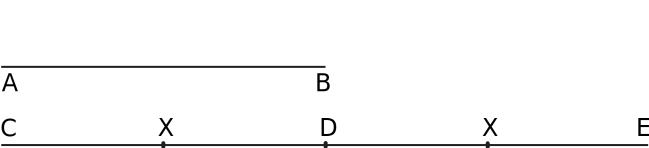
\includegraphics[width=0.55\textwidth]{gesamttex/edit_VIII,3/images/LH_37_01_001-002,003-008,025_d4a.pdf}}%\\
  \vspace{1.5em}
  \centerline{\lbrack\textit{Fig.~4a, gestr.; L\textsuperscript{1}\! (Bl.~2~v\textsuperscript{o}\!)}\rbrack}\label{LH_37_01_002v_a1.1}% 

 \vspace{4em}
  \centerline{\includegraphics[width=0.7\textwidth]{gesamttex/edit_VIII,3/images/LH_37_01_001-002,003-008,025_d4b.pdf}}%\\
  \vspace{1.5em}
  \centerline{\lbrack\textit{Fig.~4b; L\textsuperscript{1}\! (Bl.~2~v\textsuperscript{o}\!)}\rbrack}\label{LH_37_01_002v_a1}% 

  \vspace{4em}% Rein provisorisch!
  \centerline{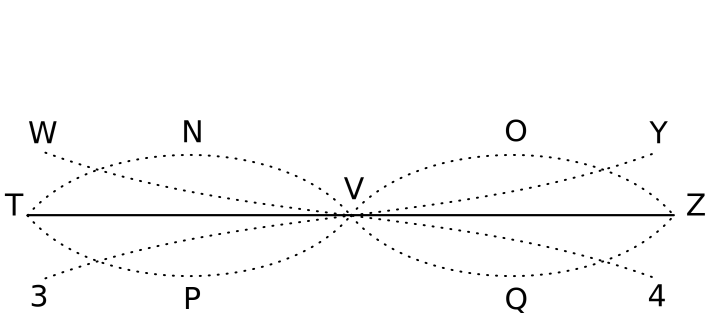
\includegraphics[width=0.57\textwidth]{gesamttex/edit_VIII,3/images/LH_37_01_001-002,003-008,025_d4c.pdf}}%
  \vspace{1.5em}
  \centerline{\lbrack\textit{Fig.~4c; L\textsuperscript{2}\! (Bl.~25~r\textsuperscript{o}\!)}\rbrack}%
%  \vspace*{1.0em}%
%  \newpage
%
%
%  \newpage
  \vspace{4em}%
  \centerline{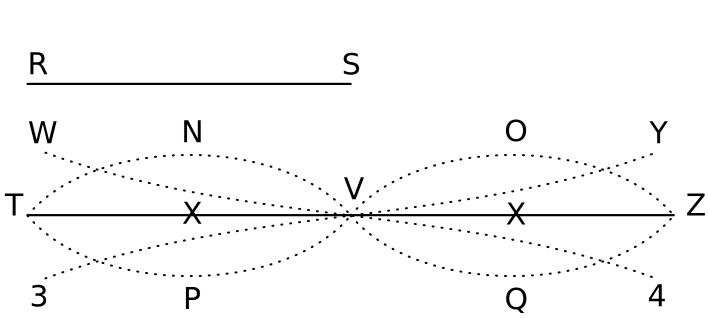
\includegraphics[width=0.58\textwidth]{gesamttex/edit_VIII,3/images/LH_37_01_001-002,003-008,025_d4d.pdf}}%\\
  \vspace{1.5em}
  \centerline{\lbrack\textit{Fig.~4d; Lil (Bl.~8~r\textsuperscript{o}\!)}\rbrack}\label{LH_37_01_008r_f-4}%
%  \vspace*{2.0em}%
  \newpage
%
%%
\count\Bfootins=900
\count\Afootins=900
\count\Cfootins=900
\pstart%
\noindent actu\protect\index{Sachverzeichnis}{actus} vel
\edtext{potentia,\protect\index{Sachverzeichnis}{potentia}
actu\protect\index{Sachverzeichnis}{actus} secundum diversas suas partes}{%
\lemma{potentia~;}\Bfootnote{\hspace{-0.5mm}% 
actu
\textit{(1)}~si constet partibus
\textit{(2)}~secundum diversas
\textit{(a)}~partes
\textit{(b)}~suas partes%
~\textit{L\textsuperscript{1}}%
\hspace{0.5mm}
potentia~, actu \lbrack...\rbrack\ suas partes%
~\textit{l}}}
%
easque rursus vel discretas\protect\index{Sachverzeichnis}{pars discreta}
vel continuas.\protect\index{Sachverzeichnis}{pars continua}
%
Discretae\protect\index{Sachverzeichnis}{pars discreta} sunt in
\edtext{lyra,\protect\index{Sachverzeichnis}{lyra}}{%
\lemma{lyra~\textit{L\textsuperscript{1}}}\Bfootnote{%
lyra~,~\textit{l}}}
%
quae potest 
\edtext{diversis aliis chordis}{%
\lemma{diversis}\Bfootnote{\hspace{0.5mm}%
\textbar~alterius \textit{erg.}~%
\textbar\ chordis%
~\textit{L\textsuperscript{1}}%
\hspace{0.5mm}
diversis
\textbar~aliis \textit{erg.~Lil}~%
\textbar\ chordis%
~\textit{l}}}
%
esse consona,
secundum diversas suas
\edtext{chordas.\protect\index{Sachverzeichnis}{chorda lyrae}
%
Aliquando continuae sunt partes;\protect\index{Sachverzeichnis}{pars continua}}{%
\lemma{chordas}\Bfootnote{\hspace{-0.5mm}%
\textbar~quae in illa sunt tensae \textit{gestr.}~\textbar~.
\textit{(1)}~Continuas,
\textit{(2)}~Aliquando continuae sunt partes,%
~\textit{L\textsuperscript{1}}%
\hspace{0.5mm}
chordas~. Aliquando continuae sunt partes;%
~\textit{l}}}
%
ita
\edtext{paulo ante}{\lemma{paulo ante}\Cfootnote{%
S.~\refpassage{LH_37_01_007v_pauloante_svdeatf-1}{LH_37_01_008r_pauloante_svdeatf-2}%
% S.~\refpassage{LH_37_01_007r_pauloante_duifzvl-1}{LH_37_01_007v_pauloante_duifzvl-2}
.}}
\edtext{ostendimus aerem,
imo et chordam proxime propositam
sponte quadam in partes\protect\index{Sachverzeichnis}{pars aeris}\protect\index{Sachverzeichnis}{pars chordae}}{%
\lemma{aerem}\Bfootnote{\hspace{-0.5mm}%
\textit{(1)}~sese in
\textit{(2)}~in partes
\textit{(3)}~, imo et chordam
\textit{(a)}~sese in partes
\textit{(b)}~novissime
\textit{(c)}~proxime propositam \lbrack...\rbrack\ in partes%
~\textit{L\textsuperscript{1}}}}
%
abire magnitudinis tantae,
ut cum data
\edtext{tensione sua\protect\index{Sachverzeichnis}{tensio chordae}\protect\index{Sachverzeichnis}{tensio aeris}
fiant dato corpori}{%
\lemma{tensione}\Bfootnote{\hspace{-0.5mm}%
\textit{(1)}~fiant alteri
\textit{(2)}~sua fiant dato corpori%
~\textit{L\textsuperscript{1}}}}
%
unisonae,\protect\index{Sachverzeichnis}{pars unisona}
\edtext{ita in \edlabel{LH_37_01_002v_gestrVarntn_wghfe-1}chorda $TZ$}{%
\lemma{ita}\Bfootnote{\hspace{-0.5mm}%
\textbar~in \textit{erg.}~%
\textbar\ chorda
\textit{(1)}~$CE$
\textit{(2)}~$TZ$%
~\textit{L\textsuperscript{1}}}}%
\edtext{}{%
{\xxref{LH_37_01_002v_gestrVarntn_wghfe-1}{LH_37_01_002v_gestrVarntn_wghfe-2}}%
{\lemma{chorda $TZ$ \lbrack...\rbrack\ $RS$ unisonae}\Cfootnote{%
In \textit{L\textsuperscript{1}} beziehen sich die gestrichenen Varianten auf das ebenfalls gestrichene Diagramm \lbrack\textit{Fig.~4a}\rbrack, S.~\pageref{LH_37_01_002v_a1.1}.}}}
%
ipso
\edtext{\lbrack consonandi\rbrack}{%
\lemma{consonandi~\textit{L\textsuperscript{1}}}\Bfootnote{% \hspace{-0.5mm}%
% \hspace{0.5mm}
sonandi \textit{l~ändert Hrsg. nach~L\textsuperscript{1}}}}
%
opere\protect\index{Sachverzeichnis}{opus consonandi}
partes
\edtext{assignantur $TV,$ $VZ,$
singulae,
ipsi $RS$ unisonae.%
\edlabel{LH_37_01_002v_gestrVarntn_wghfe-2}%
\protect\index{Sachverzeichnis}{pars unisona}}{%
\lemma{assignantur}\Bfootnote{\hspace{-0.5mm}%
\textit{(1)}~$CD,$ $DE$
\textit{(2)}~$TV,$ $VZ$
singulae ipsi
\textit{(a)}~$AB$
\textit{(b)}~$RS$ unisonae.%
~\textit{L\textsuperscript{1}}%
\hspace{0.5mm}
assignantur
\textit{(1)}~$TV.$ $VZ$~\textit{l}
\textit{(2)}~$TV,$ $VZ,$~\textit{Lil}
singulae, ipsi $RS$ unisonae.%
~\textit{l}}}
%
\edtext{Potentia denique consonum\protect\index{Sachverzeichnis}{potentia consonum}
intelligi potest unum aliis diversis,}{%
\lemma{Potentia}\Bfootnote{\hspace{-0.5mm}%
\textbar~denique \textit{erg.}~%
\textbar\ consonum
\textit{(1)}~fieri
\textit{(2)}~intelligi potest
\textit{(a)}~corpo
\textit{(b)}~unum aliis diversis,%
~\textit{L\textsuperscript{1}}}}
%
si scilicet prout opus est plus minusve tendatur
\edtext{aut laxetur.}{%
\lemma{aut}\Bfootnote{\hspace{-0.5mm}%
\hspace{-0.5mm}laxetur
\textit{erg.~L\textsuperscript{1}}}}
%
% % % %      HAKEMISTON PÄIVITYS TÄHÄN ASTI (12. huhtikuuta 2019)
%
Naturam autem cujus inimitabilis est sagacitas,\protect\index{Sachverzeichnis}{sagacitas naturae}
\edtext{arbitror omnes}{%
\lemma{arbitror~,}\Bfootnote{\hspace{-0.5mm}%
\textit{(1)}~omnia
\textit{(2)}~omnes%
~\textit{L\textsuperscript{1}}%
\hspace{0.5mm}
arbitror omnes%
~\textit{l}}}
%
modos possibiles in organo auditus\protect\index{Sachverzeichnis}{organon auditus}
\edlabel{KZeitz61}\edtext{}{{\xxref{KZeitz61}{KZeitz62}}%
{%
\lemma{conjunxisse.}\Bfootnote{\hspace{-0.5mm}%
\textit{(1)}~Primum enim cavitates
\textit{(a)}~aere
\textit{(b)}~multiplices aere implentur,
\textit{(aa)}~deinde
\textit{(bb)}~qui vibrationes externas non accipit tantum, sed et praesertim in angusto diutius.
\textit{(2)}~Nam et cavitates aere implevit, et membranam tetendit, quam tympanum vocant, et trans tympanum
\textit{(a)}~in cochlea
\textit{(b)}~in osse petroso, in primis ubi \textbar~et \textit{erg.}~%
\textbar\ cochlea est, variae magnitudinis ossicula conjunxit,
\textit{(aa)}~alia aliis
\textit{(bb)}~tonis exprimendis apta
\textit{(cc)}~majora
\textit{(dd)}~minora
\textit{(aaa)}~acutioribus
\textit{(bbb)}~celerioribus seu acutioribus, majora gravioribus tonis
\textit{(aaaa)}~exprimendis
\textit{(bbbb)}~seu vibrationibus exprimendis apta. Cum igitur \lbrack...\rbrack\ in cavitatem
\textbar~auris \textit{erg.}~%
\textbar~, primum ab aere
\textit{(aaaaa)}~incluso\protect\index{Sachverzeichnis}{aer iclusus}
\textit{(bbbbb)}~immisso exprimitur modo dicto;%
~\textit{L\textsuperscript{1}}%
\hspace{0.5mm}
con\-junxisse. Nam % et cavitates aere implevit et 
\lbrack...\rbrack\ membranam tetendit; quam
\textit{(1)}~tympanum~\textit{l}
\textit{(2)}~tympani~\textit{Lil}
vocant, et trans tympanum
\textbar~(\phantom)\hspace{-1.2mm} \textit{erg. Lil}~%
\textbar\ in
\textit{(a)}~osse petroso imprimis, ubi cochlea est,~\textit{l}
\textit{(b)}~ossis petrosi labyrintho\phantom(\hspace{-1.2mm})~\textit{Lil}
variae magnitudinis
\textit{(aa)}~oscula~\textit{l}
\textit{(bb)}~ossula
\textit{(cc)}~partes~\textit{Lil}
conjunxit;
\textit{(aaa)}~majora~\textit{l}
\textit{(bbb)}~minora
\textit{(ccc)}~minores~\textit{Lil}
celerioribus seu acutioribus,
\textit{(aaaa)}~majora~\textit{l}
\textit{(bbbb)}~majores~\textit{Lil}
gravioribus sonis seu vibrationibus exprimendis
\textit{(aaaaa)}~apta.~\textit{l}
\textit{(bbbbb)}~aptas.~\textit{Lil}
Cum igitur \lbrack...\rbrack\ in cavitatem % sonus incidit 
\textit{(aaaaa-a)}~aeris,~\textit{l}
\textit{(bbbbb-b)}~auris,~\textit{Lil}
primum ab aere
\textbar~immisso \textit{erg. Hrsg. nach~L\textsuperscript{1}}~%
\textbar\ exprimitur modo dicto,% 
~\textit{l}}}}%
conjunxisse.
\edtext{Nam et cavitates\protect\index{Sachverzeichnis}{cavitas auris}}{%
\lemma{Nam et cavitates}\Cfootnote{%
Die hier beginnende Darlegung der Anatomie des Ohres geht zum Teil auf Mariottes Aus\-füh\-run\-gen
in Briefen an Leibniz vom Jahr 1681 zurück % vom März/April 1681, vom 8. August 1681 und vom 29. November 1681
(\textit{LSB} III,~3 N.~193,\cite{01209} S.~375; N.~262,\cite{01210} S.~464; N.~297, S.~518\,f.\cite{01222}).
In dem von Leibniz neu verfassten Schlussteil (S.~\refpassage{LH_37_01_008v_g-1}{LH_37_01_008v_g-2}) wird die Beschreibung unter Berücksichtigung von N.~12\textsubscript{5} (Auszüge aus Duverneys Abhandlung über das Gehörorgan) erweitert.}}
aere\protect\index{Sachverzeichnis}{aer immissus} implevit
et membranam\protect\index{Sachverzeichnis}{membrana tympani} tetendit\lbrack,\rbrack\
quam tympani vocant,
et trans tympanum
(\phantom)\hspace{-1.2mm}%
in ossis petrosi labyrintho\protect\index{Sachverzeichnis}{labyrinthus ossis petrosi}%
\phantom(\hspace{-1.2mm})
variae magnitudinis partes conjunxit\lbrack:\rbrack\
minores celerioribus seu acutioribus,\protect\index{Sachverzeichnis}{sonus acutus}
majores gravioribus sonis\protect\index{Sachverzeichnis}{sonus gravis}
seu vibrationibus\protect\index{Sachverzeichnis}{vibratio}
exprimendis aptas.
Cum igitur sonus\protect\index{Sachverzeichnis}{sonus} incidit in
cavitatem auris,\protect\index{Sachverzeichnis}{cavitas auris}
primum ab aere\protect\index{Sachverzeichnis}{aer} \lbrack immisso\rbrack\ exprimitur modo dicto,\edlabel{KZeitz62}
%
\edtext{}{%
{\xxref{LH_37_01_008r_eirgohpiogabnp-1}{LH_37_01_008v_eirgohpiogabnp-2}}%
{\lemma{deinde \lbrack...\rbrack\ exigit}\Cfootnote{%
Siehe zu dieser Auffassung der Funktion des Trommelfells etwa
\textsc{Fabri}, \textit{Physica}, tract.~III, lib.~II, prop.~52 (Bd.~II, S.~152b\textendash153a)\cite{00044}.
Eine ähnliche Betrachtung findet sich auch in
\cite{00087}\textsc{Rohault}, \textit{Traité de physique}, partie I, chap.~26, §~48 (Bd.~I, S.~290).}}}%
\edlabel{LH_37_01_008r_eirgohpiogabnp-1}%
deinde
\edtext{tympanum\protect\index{Sachverzeichnis}{tympanum} pulsatum tenditur
%
\lbrack8~v\textsuperscript{o}\rbrack\ %%%% Blatt 8v
%
ut oportet,
et accommodat sese}{%
\lemma{tympanum}\Bfootnote{\hspace{-0.5mm}%
\textit{(1)}~aliaeque membranulae ita
\textit{(a)}~se
\textit{(b)}~tenduntur
\textit{(2)}~pulsatum
\textbar~tenditur ut oportet et \textit{erg.}~%
\textbar\ accommodat sese%
~\textit{L\textsuperscript{1}}%
\hspace{0.5mm}
tympanum pulsatum tenditur \lbrack8~v\textsuperscript{o}\rbrack\ ut oportet, %
\textbar~et accommodat \textit{erg.~Lil}~%
\textbar\ sese%
~\textit{l}}}
%
ut ejus vibrationes fiant vibrationibus aeris impingentis
\edtext{isochronae,\protect\index{Sachverzeichnis}{vibratio isochrona}
eo}{%
\lemma{isochronae,}\Bfootnote{\hspace{-0.5mm}% 
\textbar~quod fit \textit{gestr.}~\textbar\ eo%
~\textit{L\textsuperscript{1}}}}
%
naturae
\edtext{consilio\protect\index{Sachverzeichnis}{consilium naturae}}{%
\lemma{consilio~,~\textit{L\textsuperscript{1}}}\Bfootnote{%
consilio~\textit{l}}}
%
quo et humores\protect\index{Sachverzeichnis}{humor oculi}
\edtext{et partes\protect\index{Sachverzeichnis}{pars oculi} oculi}{%
\lemma{et}\Bfootnote{\hspace{-0.5mm}%
partes \textit{erg.~L\textsuperscript{1}}}}
%
\edtext{foramenque pupillae\protect\index{Sachverzeichnis}{foramen pupillae}}{%
\lemma{foramenque}\Bfootnote{\hspace{-0.5mm}%
pupillae \textit{fehlt~L\textsuperscript{1}, erg.~Lil}}}
%
a musculis\protect\index{Sachverzeichnis}{musculus} ita formari
\edtext{possunt}{%
\lemma{possunt~,~\textit{L\textsuperscript{1}}}\Bfootnote{%
possunt~\textit{l}}}
%
prout objectorum distantia\protect\index{Sachverzeichnis}{distantia objecti} aut lux\protect\index{Sachverzeichnis}{lux} exigit.\edlabel{LH_37_01_008v_eirgohpiogabnp-2}
\edlabel{LH_37_01_008v_ankn-3}%
Propagatur simul eadem
\edtext{vibratio\protect\index{Sachverzeichnis}{vibratio}
tum in aerem\protect\index{Sachverzeichnis}{aer inclusus}
trans\edlabel{LH_37_01_002v_txtvrlst-1} membranam tympani,\protect\index{Sachverzeichnis}{membrana tympani}
tum in ossicula\protect\index{Sachverzeichnis}{ossicula auris}
\edlabel{LH_37_01_008v_ankn-1}multiplicia\edlabel{LH_37_01_008v_ankn-2}}{%
\lemma{vibratio}\Bfootnote{\hspace{-0.5mm}%
in aerem trans $\langle$tympanum$\rangle$ % \textendash
\textit{(1)}~in
\textit{(2)}~ad ossa multiplicia%
~\textit{L\textsuperscript{1}}%
\hspace{0.5mm}
vibratio
\textit{(1)}~in aere trans tympanum in ossa~\textit{l}
\textit{(2)}~tum in \lbrack...\rbrack\ in ossicula~\textit{Lil}
multiplicia%
~\textit{l}}}
%
\pend%
% \newpage%
\vspace{0.5em}
\pstart%
\noindent%
\lbrack\textit{Nachfolgend kleingedruckten Textabschnitt, mit dem die Reinschrift \textit{l} endet, hat Leibniz zunächst über\-ar\-bei\-tet, dann gestrichen und durch neue Fassungen (S.~\refpassage{LH_37_01_008v_ersteSchlussersetzung_rfvp-1}{LH_37_01_008v_ersteSchlussersetzung_rfvp-2}; \refpassage{LH_37_01_008v_g-1}{LH_37_01_008v_g-2}) ersetzt:}\rbrack\
\pend%
\vspace{0.5em}
\footnotesize%
\pstart%
\noindent%
%<t-1>
\edtext{\edlabel{LH_37_01_008v_gestrSchluss_fuwi-1}ubi omnes particulae}{%
\lemma{$\langle$ub$\rangle$i}\Bfootnote{\hspace{-0.5mm}%
\textit{(1)}~omnia illa ossicula\protect\index{Sachverzeichnis}{ossicula auris}
\textit{(2)}~omnes illae particulae%
~\textit{L\textsuperscript{1}}%
\hspace{0.5mm}
ubi omnes
\textbar~illae \textit{fehlt}~%
\textbar\ particulae%
~\textit{l}}}
%
quae debitae sunt magnitudinis
\edtext{(\phantom)\hspace{-1.2mm}%
coeunt enim quasi ex amplo in arctum
instar tubarum\protect\index{Sachverzeichnis}{tuba}
atque ita varios gradus exhibent%
\phantom(\hspace{-1.2mm})}{%
\lemma{(\phantom)\hspace{-1.2mm}coeunt}\Bfootnote{\hspace{-0.5mm}%
enim quasi
\textit{(1)}~in arctum
\textit{(2)}~ex amplo in arctum atque ita varios gradus exhibent\phantom(\hspace{-1.2mm})
\textit{erg.~L\textsuperscript{1}}%
\hspace{0.5mm}
(\phantom)\hspace{-1.2mm}coeunt enim % quasi ex amplo 
\lbrack...\rbrack\ in arctum
\textbar~instar tubarum \textit{erg. Lil}~%
\textbar\ atque ita varios gradus exhibent\phantom(\hspace{-1.2mm})%
~\textit{l}}}
%
easdem accipiunt
\edtext{vibrationes\protect\index{Sachverzeichnis}{vibratio ossiculorum auris}
quae tum mutuo suas}{%
\lemma{vibra$\langle$tiones}\Bfootnote{\hspace{-0.5mm}%
quae tum aeris incl$\rangle$usi%
~\textit{L\textsuperscript{1}}%
\hspace{0.5mm}
vibrationes quae tum
\textit{(1)}~aeris inclusi\protect\index{Sachverzeichnis}{vibratio aeris inclusi}~\textit{l}
\textit{(2)}~mutuo suas%
~\textit{Lil}}}
%
vibrationes juvant et conservant\protect\index{Sachverzeichnis}{conservatio vibrationis}
tum etiam fortasse ita propagant\protect\index{Sachverzeichnis}{propagatio vibrationis}
\edtext{sonumque\protect\index{Sachverzeichnis}{sonus} quodammodo reflectunt,\protect\index{Sachverzeichnis}{reflexio soni}%
}{%
\lemma{$\langle$sonumque}\Bfootnote{\hspace{-0.5mm}%
quodammodo reflectunt$\rangle$%
~\textit{L\textsuperscript{1}}}}
%
et in
\edtext{unum dirigunt,
ut}{%
\lemma{unum}\Bfootnote{\hspace{-0.5mm}%
\textit{(1)}~cogunt
\textit{(2)}~dirigunt, $\langle$ut$\rangle$%
~\textit{L\textsuperscript{1}}}}
%
omnium
\edtext{conspirante nisu\protect\index{Sachverzeichnis}{nisus conspirans}}{%
\lemma{conspi$\langle$rante}\Bfootnote{\hspace{-0.5mm}%
n$\rangle$isu%
~\textit{L\textsuperscript{1}}}}%
\edlabel{LH_37_01_002v_txtvrlst-2}
%
ultimum
\edtext{sensorium\protect\index{Sachverzeichnis}{sensorium ultimum}
(\phantom)\hspace{-1.1mm}%
sive}{%
\lemma{sensorium}\Bfootnote{\hspace{-0.5mm}%
sive~\textit{L\textsuperscript{1}}%
\hspace{0.5mm}
sensorium
\textbar~(\phantom)\hspace{-1.1mm} \textit{erg.~Lil}~%
\textbar\ sive~\textit{l}}}
%
id sit nervus
\edtext{acusticus\protect\index{Sachverzeichnis}{nervus acusticus} sive alius}{%
\lemma{acusticus}\Bfootnote{\hspace{-0.5mm}%
sive \textbar~potius \textit{gestr.}~\textbar\ alius%
~\textit{L\textsuperscript{1}}}}
%
quidam
\edtext{plexus\protect\index{Sachverzeichnis}{plexus}%
\phantom(\hspace{-1.1mm})
iisdem}{%
\lemma{plexus}\Bfootnote{\hspace{-0.5mm}%
\textbar~aut membrana\protect\index{Sachverzeichnis}{membrana}
\textit{gestr.}~\textbar\ iisdem%
~\textit{L\textsuperscript{1}}%
\hspace{0.5mm}
plexus
\textbar~\phantom(\hspace{-1.1mm}) \textit{erg.~Lil}~%
\textbar\ iisdem%
~\textit{l}}}
%
vibrationibus\protect\index{Sachverzeichnis}{vibratio} satis
\edtext{notabiliter}{%
\lemma{notabiliter}\Bfootnote{\hspace{-0.5mm}%
\textit{fehlt~L\textsuperscript{1}, erg.~Lil}}}
afficiatur,\protect\index{Sachverzeichnis}{affectio sensorii}
atque ita denique impressio\protect\index{Sachverzeichnis}{impressio soni} eadem
ad cerebrum\protect\index{Sachverzeichnis}{cerebrum} ipsum traducatur.%
\edlabel{LH_37_01_008v_gestrSchluss_fuwi-2}%
\pend%
% \newpage%
\vspace{0.5em}
%
%
\normalsize%
\pstart%
\noindent%
\lbrack\textit{Nachfolgend kleingedruckter Textabschnitt, den Leibniz quer am Rand von Bl.~2~v\textsuperscript{o}\! als ursprünglichen Schluss des Konzeptes L\textsuperscript{1}\! verfasst hatte, wurde nicht in die Reinschrift \textit{l} abgeschrieben:}\rbrack\
\pend%
\vspace{0.5em}
\footnotesize%
\pstart%
\noindent%
Quicquid\edlabel{LH_37_01_002v_Schluss-1}
enim moliamur\lbrack,\rbrack\
huc tandem veniendum est,
ut tum omnes vibrationes partium organi\protect\index{Sachverzeichnis}{vibratio organi auditus}
sono\protect\index{Sachverzeichnis}{sonus} percussarum fiant
\edtext{quoad licet}{%
\lemma{quoad}\Bfootnote{\hspace{-0.5mm}%
licet
\textit{erg.~L\textsuperscript{1}}}}
%
isochronae\protect\index{Sachverzeichnis}{vibratio isochrona}
vibrationibus rei sonantis,\protect\index{Sachverzeichnis}{vibratio rei sonantis}
tum, ut omnes denique vibrationes illae
quantum satis est
ad ultimum illud in quo sensus fit % \lbrack,\rbrack\
quem
\edtext{communem\protect\index{Sachverzeichnis}{sensus communis} vocant}{%
\lemma{communem vocant}\Cfootnote{%
Siehe etwa \textsc{Aristoteles}, \textit{De anima} III 1, 425a27.\cite{01217}}}%
\lbrack,\rbrack\
convergant
\edtext{et vim\protect\index{Sachverzeichnis}{vis vibrationis}
propagent,\protect\index{Sachverzeichnis}{propagatio vibrationis}}{%
\lemma{et}\Bfootnote{\hspace{-0.5mm}%
\textit{(1)}~propagentur
\textit{(2)}~vim propagent,%
~\textit{L\textsuperscript{1}}}}
%
quod solidumne\protect\index{Sachverzeichnis}{solidum}
an fluidum\protect\index{Sachverzeichnis}{fluidum} sit nondum hic
\edlabel{KZeitz63}\edtext{}{{\xxref{KZeitz63}{KZeitz64}}%
{%
\lemma{definiemus.}\Bfootnote{\hspace{-0.5mm}%
\textit{(1)}~Ex his meditationibus excerpta
\textit{(2)}~Harum meditationum compendium
\textit{(a)}~intellexi
\textit{(b)}~cum observationibus quoque nuperis
\textit{(aa)}~Lutetiae Parisiorum\protect\index{Ortsregister}{Paris} sumtis, ratio
\textit{(bb)}~ibi sumtis ac superstructis sententiis
\textit{(cc)}~quas praeclaros
\textbar~quosdam \textit{erg.}~\textbar\ Academiae illae \lbrack...\rbrack\ publicare accepi
\textit{(aaa)}~quemadmodum a Cl. Mariotto,%
\protect\index{Namensregister}{\textso{Mariotte}, Edme, Seigneur de Chazeuil ca. 1620\textendash1684} cujus pariter et
\textit{(aaaa)}~Duvernaei
\textit{(aaaaa)}~$\langle$\textendash\,ac\,\textendash$\rangle$
\textit{(bbbbb)}~cogitata
\textit{(aaaaa-a)}~in
\textit{(bbbbb-b)}~cum
\textit{(bbbb)}~diligentissimi Duvernaei\protect\index{Namensregister}{\textso{Duverney} (Duvernejus, Duvernaeus), Joseph-Guichard 1648\textendash1730} egregia
\textit{(cccc)}~accurata Duvernaei descriptione auris \textbar~primum \textit{erg.}~\textbar\ habebamus,
\textit{(bbb)}~egregie consentire intellexi.%
~\textit{L\textsuperscript{1}}}}}%
definiemus.
\edtext{Harum meditationum\protect\index{Sachverzeichnis}{meditatio}}{%
\lemma{Harum meditationum}\Cfootnote{%
Als Leibniz am 28. April 1682 an C.~Pfautz mitteilte,
\textit{quaedam Meditationes} über die Akustik in den \textit{AE} veröffentlichen zu wollen
(\cite{01281}\textit{LSB} III,~3 N.~345, S.~596.20\textendash597.1),
bezog er sich wohl auf \textit{L\textsuperscript{1}}.
Leibniz hat den Aufsatz nie veröffentlicht.}}
\edtext{compendium\protect\index{Sachverzeichnis}{compendium}}{%
\lemma{compendium}\Cfootnote{%
In \textit{L\textsuperscript{1}} findet sich an dieser Stelle ein Einfügungszeichen, das sich nicht zuordnen lässt.}}
cum observationibus\protect\index{Sachverzeichnis}{observatio} quoque nuperis
quas
\edtext{praeclaros quosdam Academiae illae Regiae%
\protect\index{Sachverzeichnis}{Académie Royale des Sciences}
viros\protect\index{Sachverzeichnis}{vir} publicare accepi}{%
\lemma{praeclaros \lbrack...\rbrack\ accepi}\Cfootnote{%
Vermutlich Anspielung auf Vorträge über die Anatomie und Physiologie des Gehörorganes,
die Mariotte und Duverney 1681 vor der Pariser Akademie der Wissenschaften hielten.
Siehe E.~\textsc{Mariotte}, Briefe an G.\,W. Leibniz vom März/April und vom 8. August 1681
(\textit{LSB} III,~3 N.~193, S.~375\cite{01209}; N.~262, S.~464\cite{01210}).
Ein Kurzbericht über Duverneys Forschungsergebnisse wurde auch in \textit{JS}, 23. Juni 1681 (% Nr.~17, 
Pariser Ausgabe: S.~214\textendash216\cite{01211}) veröffentlicht.}}%
\lbrack,\rbrack\
\edtext{egregie consentire intellexi.\edlabel{LH_37_01_002v_Schluss-2}%
}{\lemma{egregie consentire intellexi}\Cfootnote{% consentire
Siehe E.~\textsc{Mariotte}, Brief an G.\,W. Leibniz vom 29. November 1681 (\textit{LSB} III,~3 N.~297, S.518\,f.\cite{01222}).
Dort hebt Mariotte die Übereinstimmung von Leibnizens Ansichten über die Akustik mit seinen eigenen hervor.}}\edlabel{KZeitz64}%
%%
\pend%
\vspace{0.5em}%
% \newpage%
%
\normalsize%
\pstart%
\noindent%
\lbrack\textit{Nachfolgend kleingedruckten Textabschnitt hat Leibniz am Rand von Bl.~8~v\textsuperscript{o}\!
als erste Ersetzung für den gestrichenen Schlussteil der Reinschrift \textit{l} (S.~\refpassage{LH_37_01_008v_gestrSchluss_fuwi-1}{LH_37_01_008v_gestrSchluss_fuwi-2})
verfasst und dann gestrichen (\textit{Lil}):}\rbrack\ 
\pend%
\vspace{0.5em}%
\footnotesize%
\pstart%
\noindent%
%<t-2>
\footnotesize%
nempe\edlabel{LH_37_01_008v_ersteSchlussersetzung_rfvp-1}
\edtext{a membrana tympani\protect\index{Sachverzeichnis}{membrana tympani}}{%
\lemma{a}\Bfootnote{\hspace{-0.5mm}%
\textit{(1)}~tympano
\textit{(2)}~membrana tympani%
~\textit{Lil}}}
%
in malleum\protect\index{Sachverzeichnis}{malleus} annexum\lbrack,\rbrack\
ab hoc in incudem,\protect\index{Sachverzeichnis}{incus} inde in stapedem\protect\index{Sachverzeichnis}{stapes}
qui foramen ovale\protect\index{Sachverzeichnis}{foramen ovale} in os petrosum\protect\index{Sachverzeichnis}{os petrosum} tendens
base sua exacte claudit ope membranae\protect\index{Sachverzeichnis}{membrana foraminis ovalis} annatae,
et tum interioribus partibus ossis petrosi,\protect\index{Sachverzeichnis}{os petrosum}
huic foramini\protect\index{Sachverzeichnis}{foramen ovale} propinquis,
nempe
\edtext{canalibus in semicirculum flexis,\protect\index{Sachverzeichnis}{canales semicirculares}}{%
\lemma{canalibus}\Bfootnote{\hspace{-0.5mm}%
\textit{(1)}~semicirculum flexis
\textit{(2)}~in semicirculum flexis,%
~\textit{Lil}}}
%
tum aeri iis incluso\protect\index{Sachverzeichnis}{aer inclusus}
\edtext{\lbrack communicatur\rbrack.}{%
\lemma{communicat}\Bfootnote{\textit{Lil~ändert Hrsg.}}}
%
Et rursus ab aere trans membranam tympani\protect\index{Sachverzeichnis}{membrana tympani} ad membranae
\edtext{hujus\protect\index{Sachverzeichnis}{membrana tympani}}{%
\lemma{hujus}\Bfootnote{\hspace{-0.5mm}%
\textit{erg.~Lil}}}
%
imitationem\protect\index{Sachverzeichnis}{imitatio} vibrante,
vibratio\protect\index{Sachverzeichnis}{vibratio} propagatur tum in dicta ossicula,\protect\index{Sachverzeichnis}{ossicula auris}
tum praeterea in membranam\protect\index{Sachverzeichnis}{membrana foraminis rotundi}
(\phantom)\hspace{-1.2mm}membranae tympani\protect\index{Sachverzeichnis}{membrana tympani}
\edtext{similem\phantom(\hspace{-1.2mm})
foramini rotundo\protect\index{Sachverzeichnis}{foramen rotundum} in osse petroso\protect\index{Sachverzeichnis}{os petrosum} obtensam,
per quam}{%
\lemma{similem\phantom(\hspace{-1.2mm})}\Bfootnote{\hspace{-0.5mm}%
\textit{(1)}~foraminis rotundi, qua et
\textit{(2)}~foramini rotundo \lbrack...\rbrack\ per quam%
~\textit{Lil}}}
%
aer trans hanc membranam\protect\index{Sachverzeichnis}{membrana foraminis rotundi} in ossis petrosi cavitate
\edtext{seu cochlea\protect\index{Sachverzeichnis}{cochlea}
(\phantom)\hspace{-1.2mm}parte labyrinthi\protect\index{Sachverzeichnis}{labyrinthus ossis petrosi}\phantom(\hspace{-1.2mm})}{%
\lemma{seu}\Bfootnote{\hspace{-0.5mm}%
\textit{(1)}~labyrintho
\textit{(2)}~cochlea (\phantom)\hspace{-1.2mm}parte labyrinthi\phantom(\hspace{-1.2mm})%
~\textit{Lil}}}
%
inclusus\protect\index{Sachverzeichnis}{aer inclusus}
pariter ac ipse cochleae canalis\protect\index{Sachverzeichnis}{canalis cochleae} ad vibrandum incitatur.
Et vero lamina quaedam spiralis cochleam\protect\index{Sachverzeichnis}{lamina cochleae}
in duas quasi scalas\protect\index{Sachverzeichnis}{scalae cochleatae} duplicis ascensus inter se non communicantes dividit,
quarum una est super alteram,
\edtext{et superior communicat}{%
\lemma{et}\Bfootnote{\hspace{-0.5mm}%
\textit{(1)}~superior quidem commu
\textit{(2)}~superior communicat%
~\textit{Lil}}}
%
cum aere intra canales semicirculares\protect\index{Sachverzeichnis}{canales semicirculares} ossis petrosi\protect\index{Sachverzeichnis}{os petrosum}\edlabel{LH_37_01_008v_ersteSchlussersetzung_rfvp-2}
\normalsize{\lbrack\textit{Text bricht ab.}\rbrack}
\pend%
\newpage%
%\vspace{0.5em}%
%
%
\normalsize%
\pstart%
\noindent%
\lbrack\textit{Nachfolgenden, das Konzept L\textsuperscript{2}\! mit Verbesserungen wiedergebenden Textabschnitt (bis~zu S.~\refpassage{LH_37_01_008v_h-1}{LH_37_01_008v_h-2})
hat Leibniz am Rand von Bl.~8~v\textsuperscript{o}\!
als zweite, gültige Ersetzung für den gestri\-chenen Schlussteil der Reinschrift \textit{l} (S.~\refpassage{LH_37_01_008v_gestrSchluss_fuwi-1}{LH_37_01_008v_gestrSchluss_fuwi-2}) abgefasst (\textit{Lil}):}\rbrack\ 
\pend%
\vspace{0.5em}%
\pstart%
\noindent%
%<t-3>
trans\edlabel{LH_37_01_008v_g-1} eandem
\edtext{membranam}{%
\lemma{membranam}\Bfootnote{\hspace{-0.5mm}%
\textit{fehlt~L\textsuperscript{2}, erg.~Lil}}}
%
in tympano posita,\protect\index{Sachverzeichnis}{membrana tympani}
%%
\edtext{membranae ipsi\protect\index{Sachverzeichnis}{membrana tympani} connexa;
malleum,\protect\index{Sachverzeichnis}{malleus} incudem\protect\index{Sachverzeichnis}{incus} et stapedem.\protect\index{Sachverzeichnis}{stapes}
Inde denique pervenit vibratio\protect\index{Sachverzeichnis}{vibratio}
in labyrinthum in osse petroso excavatum,\protect\index{Sachverzeichnis}{labyrinthus ossis petrosi}
idque tum per tremores\protect\index{Sachverzeichnis}{tremor} ipsius ossis petrosi,\protect\index{Sachverzeichnis}{os petrosum}
tum per\textso{ foramina }in osse petroso.
Ipsum os petrosum\protect\index{Sachverzeichnis}{os petrosum} tremit
ad imitationem\protect\index{Sachverzeichnis}{imitatio} membranae tympani,\protect\index{Sachverzeichnis}{membrana tympani}
tum ob vibrationes aeris\protect\index{Sachverzeichnis}{vibratio aeris} inter ipsum et membranam hanc positi
a membranae\protect\index{Sachverzeichnis}{membrana tympani} pulsatione\protect\index{Sachverzeichnis}{pulsatio}
per aerem externum\protect\index{Sachverzeichnis}{aer externus} facta, incitati;
tum ob tremores\protect\index{Sachverzeichnis}{tremor} ossiculorum dictorum\protect\index{Sachverzeichnis}{ossicula auris}
inter membranam\protect\index{Sachverzeichnis}{membrana tympani} et os petrosum\protect\index{Sachverzeichnis}{os petrosum}
interjectorum, nam
malleus\protect\index{Sachverzeichnis}{malleus} membranae tympani,\protect\index{Sachverzeichnis}{membrana tympani}
stapes\protect\index{Sachverzeichnis}{stapes} ossi petroso\protect\index{Sachverzeichnis}{os petrosum} connectitur,
incus\protect\index{Sachverzeichnis}{incus} eos jungit, unde communicatio.%
\textso{ Foramina }in osse petroso qua tympanum\protect\index{Sachverzeichnis}{tympanum} respicit
sunt ovale\protect\index{Sachverzeichnis}{foramen ovale} et rotundum.\protect\index{Sachverzeichnis}{foramen rotundum}
Ovale\protect\index{Sachverzeichnis}{foramen ovale} clauditur a stapede\protect\index{Sachverzeichnis}{stapes}
cujus basis membrana adnata\protect\index{Sachverzeichnis}{membrana foraminis ovalis} jungitur orae foraminis.
Rotundum clauditur propria membrana\protect\index{Sachverzeichnis}{membrana foraminis rotundi}}{%
\lemma{membranae}\Bfootnote{\hspace{-0.5mm}%
tympani
\textit{(1)}~connexa
\textit{(2)}~connexa,
\textbar~malleum incudem et stapedem \textit{erg.}~%
\textbar\ inde denique
\textit{(a)}~propagatio\protect\index{Sachverzeichnis}{propagatio soni}
\textit{(b)}~pervenit vibratio in
\textit{(aa)}~aerem inclusum ossi petroso,\protect\index{Sachverzeichnis}{aer inclusus}
\textit{(bb)}~laminas\protect\index{Sachverzeichnis}{lamina cochleae}
\textit{(cc)}~canales et\protect\index{Sachverzeichnis}{canales semicirculares}
\textit{(aaa)}~laminas
\textit{(bbb)}~Cochleam labyrinthi in osse petroso excavati quod fit per duo foramina
\textit{(dd)}~\textbar~in \textit{versehentlich erhalten}~%
\textbar\ labyrinthum in osse petroso excavatum
\textit{(aaa)}~aeremque ei inclusum, quem Anatomici veteres\protect\index{Sachverzeichnis}{anatomici veteres} vocabant implantatum\protect\index{Sachverzeichnis}{aer implantatus}
\textit{(bbb)}~, idque
\textit{(aaaa)}~per duo foramina, unum rotundum\protect\index{Sachverzeichnis}{foramen rotundum} membrana\protect\index{Sachverzeichnis}{membrana foraminis rotundi} clausum quam
\textit{(aaaaa)}~inter
\textit{(bbbbb)}~inter tympani membranam\protect\index{Sachverzeichnis}{membrana tympani} et os petrosum
\textit{(ccccc)}~inter
\textit{(ddddd)}~positus\lbrack\textit{!}\rbrack\
\textit{(bbbb)}~tum per
\textit{(aaaaa)}~vibrationem
\textit{(bbbbb)}~vibrationes
\textit{(ccccc)}~tremorem ipsius ossis petrosi
\textit{(aaaaa-a)}~ab aere inter ipsum et membranam tympani intercepto, tum
\textit{(bbbbb-b)}~qui et ab aere inter ipsum et membranam tympani intercepto, et per
\textit{(aaaaa-aa)}~stapedem ipsi
\textit{(bbbbb-bb)}~malleum membranis tym\protect\index{Sachverzeichnis}{membrana tympani}
\textit{(ccccc-c)}~\textbar~superficiei \textit{erg.}~%
\textbar\ tum
\textbar~maxime \textit{erg.}~%
\textbar\ per foramina % in osse petroso. Ipsum os 
\lbrack...\rbrack\ petrosum tremit
\textbar~ad imitationem tympani \textit{erg.}~%
\textbar\ tum ob vibrationes % aeris inter ipsum 
\lbrack...\rbrack\ et membranam tympani positi, tum ob tremores ossiculorum interceptorum, nam malleus
% membranae tympani, stapes ossi 
\lbrack...\rbrack\ petroso connectitur incus eos iungit. Foramina in osse petroso
\textit{(aaaaa-aa)}~sunt
\textit{(bbbbb-bb)}~qua tympanum respicit, % sunt ovale et 
\lbrack...\rbrack\ rotundum. Ovale
\textit{(aaaaa-aaa)}~et
\textit{(bbbbb-bbb)}~clauditur a stapede
\textit{(aaaaa-aaaa)}~ope membranae adnatae rotun
\textit{(bbbbb-bbbb)}~cujus basis % membrana adnata jungitur
\lbrack...\rbrack\ orae foraminis.
\textit{(aaaaa-aaaaa)}~Foramen
\textit{(bbbbb-bbbbb)}~Rotundum clauditur propria membrana,%
~\textit{L\textsuperscript{2}}%
\hspace{0.5mm}
membranae ipsi \lbrack...\rbrack\ petrosum interjectorum,
\textit{(1)}~cum
\textit{(2)}~nam malleus
\lbrack...\rbrack\ propria membrana%
~\textit{Lil}}}
%%
quae membranae tympani\protect\index{Sachverzeichnis}{membrana tympani} similis est.
Labyrinthus intra os petrosum\protect\index{Sachverzeichnis}{labyrinthus ossis petrosi} undique conclusus
%%%%
\edtext{constat potissimum tribus canalibus in semicirculum inflexis,\protect\index{Sachverzeichnis}{canales semicirculares} et cochlea.
Cochleae autem canalis\protect\index{Sachverzeichnis}{canalis cochleae}
a lamina\protect\index{Sachverzeichnis}{lamina cochleae} quadam
(\phantom)\hspace{-1.2mm}%
axem cochleae spiraliter circumeunte atque interiore sua acie,
ut ita dicam, ad axem cochleae annata,
exteriore vero per membranam quandam parieti canalis,\protect\index{Sachverzeichnis}{canalis cochleae}
in quo
\lbrack excavata cochlea\rbrack\
est, adhaerente\phantom(\hspace{-1.2mm})
dividitur}{%
\lemma{constat}\Bfootnote{% \hspace{-0.5mm}%
\textit{(1)}~vestibulo et cochlea
\textit{(2)}~potissimum \textbar~tribus \textit{erg.}~\textbar\ canalibus in % semicirculum inflexis, 
\lbrack...\rbrack\ et cochlea.
\textit{(a)}~Cochlea autem dividitur a
\textit{(b)}~Cochleae autem \lbrack...\rbrack\ spiraliter circumeunte
\textit{(aa)}~et in summo coarctata dividitur
\textit{(bb)}~atque
\textit{(aaa)}~basi sua
\textit{(bbb)}~interiore
\textit{(aaaa)}~parte sui
\textit{(bbbb)}~sua acie ad axem cochleae annata, exteriore \textbar~vero \textit{erg.}~\textbar\ per membranam
\textit{(aaaaa)}~ossi pe
\textit{(bbbbb)}~parieti canalis
\textit{(aaaaa-a)}~cui
\textit{(bbbbb-b)}~in quo excavata cochlea est, adhaerente\phantom(\hspace{-1.2mm}) dividitur%
~\textit{L\textsuperscript{2}}%
\hspace{0.5mm}
constat potissimum \lbrack...\rbrack\ lamina quadam (\phantom)\hspace{-1.2mm}~%
\textbar~extensa et \textit{gestr.}~\textbar\ axem cochleae \lbrack...\rbrack\ in quo
\textbar~excavatus \textit{ändert Hrsg. nach~L\textsuperscript{2}}~%
\textbar\ est, adhaerente\phantom(\hspace{-1.2mm}) dividitur%
~\textit{Lil}}}
%%%%
in duas quasi
\edtext{scalas\protect\index{Sachverzeichnis}{scalae cochleatae} (\phantom)\hspace{-1.2mm}seu duplicem ascensum\phantom(\hspace{-1.2mm}) quarum}{%
\lemma{scalas}\Bfootnote{\hspace{-0.5mm}%
(\phantom)\hspace{-1.2mm}seu duplicem ascensum,\phantom(\hspace{-1.2mm}) quarum%
~\textit{L\textsuperscript{2}}%
\hspace{0.5mm}
scalas
\textit{(1)}~quarum
\textit{(2)}~(\phantom)\hspace{-1.2mm}seu duplicem ascensum\phantom(\hspace{-1.2mm}) quarum%
~\textit{Lil}}}
%
una cum altera non communicat
etsi una super alia
\edtext{sit,}{%
\lemma{sit~\textit{L\textsuperscript{2}}}\Bfootnote{%
sit~,~\textit{Lil}}}
%
solaque lamina\protect\index{Sachverzeichnis}{lamina cochleae} dividantur.
Horum ascensuum superior communicat cum aere canalium
\edtext{semicircularium,\protect\index{Sachverzeichnis}{canales semicirculares}
qui vibrationem\protect\index{Sachverzeichnis}{vibratio}
\lbrack recepere\rbrack,
tum ab ipso tremore\protect\index{Sachverzeichnis}{tremor} ossis petrosi,
tum a stapede\protect\index{Sachverzeichnis}{stapes} per foramen ovale.\protect\index{Sachverzeichnis}{foramen ovale}
At inferioris ascensus sive meatus\protect\index{Sachverzeichnis}{meatus cochleae} aer,\protect\index{Sachverzeichnis}{aer inclusus} cum}{%
\lemma{semicircularium}\Bfootnote{\hspace{-0.5mm}%
\textit{(1)}~; inferior cum
\textit{(2)}~qui vibrationem recepere
\textit{(a)}~tum a superficie
\textit{(b)}~tum ab ipsa superficie ossis petrosi, \lbrack...\rbrack\ foramen ovale; inferioris ascensus aer, cum%
~\textit{L\textsuperscript{2}}%
\hspace{0.5mm}
semicircularium, qui vibrationem
\textbar~accessere \textit{ändert Hrsg. nach~L\textsuperscript{2}}~%
\textbar~, tum ab ipso \lbrack...\rbrack\ meatus aer, cum%
~\textit{Lil}}}
%
nullo alio immediate
\edtext{communicat,
vibrationem vero accepit
% \edtext{\lbrack accipit\rbrack}{%
% \lemma{accepit}\Bfootnote{%
% \textit{Lil~ändert Hrsg. nach \textit{L\textsuperscript{2}}, S.~\refpassage{LH_37_01_025r_accip-1}{LH_37_01_025r_accip-2}}}}
tum a dicto tremore\protect\index{Sachverzeichnis}{tremor}}{%
\lemma{communicat,}\Bfootnote{\hspace{-0.5mm}%
et vibrationem
\textit{(1)}~accepit
\textit{(2)}~accipit
\textit{(a)}~tum eti
\textit{(b)}~cum
\textit{(c)}~tum a dicta superficie%
~\textit{L\textsuperscript{2}}%
\hspace{0.5mm}
communicat, vibrationem \lbrack...\rbrack\ dicto tremore% vero accepit tum a
~\textit{Lil}}}
%
ossis petrosi,\protect\index{Sachverzeichnis}{os petrosum}
tum a membrana foraminis rotundi,\protect\index{Sachverzeichnis}{membrana foraminis rotundi}
quam aeris\protect\index{Sachverzeichnis}{aer inclusus} intra tympanum et os petrosum
\edtext{positi}{%
\lemma{positi}\Bfootnote{\hspace{-0.5mm}%
\textit{fehlt~L\textsuperscript{2}, erg.~Lil}}}
%
vibratio,\protect\index{Sachverzeichnis}{vibratio aeris}
ad imitationem\protect\index{Sachverzeichnis}{imitatio} membranae tympani\protect\index{Sachverzeichnis}{membrana tympani}
in tremorem\protect\index{Sachverzeichnis}{tremor} concitavit.
Lamina\protect\index{Sachverzeichnis}{lamina cochleae} autem
\edtext{cochleae}{%
\lemma{cochleae}\Bfootnote{\hspace{-0.5mm}%
\textit{fehlt~L\textsuperscript{2}}}}
%
inter hos duos
\edtext{ascensus seu meatus intercepta,}{%
\lemma{ascensus}\Bfootnote{\hspace{-0.5mm}%
\textbar~seu meatus \textit{erg.}~%
\textbar\ intercepta%
~\textit{L\textsuperscript{2}}%
\hspace{0.5mm}
ascensus seu meatus intercepta,%
~\textit{Lil}}}
%
tum a superioris tum ab
\edtext{inferioris meatus\protect\index{Sachverzeichnis}{meatus cochleae} aere}{%
\lemma{inferioris}\Bfootnote{\hspace{-0.5mm}%
aeris vibrationibus%
~\textit{L\textsuperscript{2}}%
\hspace{0.5mm}
inferioris meatus aere%
~\textit{Lil}}}
%
\edtext{pulsatur.
Unde patet quoque
cur dentibus\protect\index{Sachverzeichnis}{dens} manubrium barbiti\protect\index{Sachverzeichnis}{manubrium barbiti} apprehendentes
sonum percipiamus,\protect\index{Sachverzeichnis}{perceptio soni}
etiam auribus\protect\index{Sachverzeichnis}{auris} obturatis,
quod per mandibulae\protect\index{Sachverzeichnis}{mandibula} et temporum\protect\index{Sachverzeichnis}{tempus} ossa
tremor\protect\index{Sachverzeichnis}{tremor} ossiculis supradictis\protect\index{Sachverzeichnis}{ossicula auris}
et ita per stapedem\protect\index{Sachverzeichnis}{stapes} ossi petroso communicatur.
Caeterum cum canales semicirculares,\protect\index{Sachverzeichnis}{canales semicirculares}
tum}{%
\lemma{pulsatur.}\Bfootnote{\hspace{-0.5mm}%
\textit{(1)}~Caeterum et canales et
\textit{(2)}~Unde patet \lbrack...\rbrack\ sonum percipiamus, quod
\textbar~per \textit{versehentlich gestr.}~%
\textbar\ os mandibulae et temporum ossa \lbrack...\rbrack\ communicatur. Caeterum tum canales semicirculares tum%
~\textit{L\textsuperscript{2}}%
\hspace{0.5mm}
pulsatur. Unde \lbrack...\rbrack\ semicirculares, tum%
~\textit{Lil}}}
%
cochleae
\edtext{meatus\protect\index{Sachverzeichnis}{meatus cochleae} et lamina,\protect\index{Sachverzeichnis}{lamina cochleae}}{%
\lemma{meatus}\Bfootnote{\hspace{-0.5mm}%
cum lamina%
~\textit{L\textsuperscript{2}}%
\hspace{0.5mm}
meatus et lamina,%
~\textit{Lil}}}
%
coeunt
\edtext{ex amplo}{%
\lemma{ex}\Bfootnote{%\hspace*{-0.5mm}%
amplo~\textit{fehlt~L\textsuperscript{2}}}}
in arctum instar tubarum,\protect\index{Sachverzeichnis}{tuba}
\edtext{unde partes sive gyri minores facilius exprimunt sonos acutiores,\protect\index{Sachverzeichnis}{sonus acutus}
ampliores vero gyri exprimunt sonos graviores,\protect\index{Sachverzeichnis}{sonus gravis}}{%
\lemma{unde}\Bfootnote{\hspace{-0.5mm}%
\textit{(1)}~partium
\textit{(2)}~partes arctiores
\textit{(a)}~ad acutiores
\textit{(b)}~facilius exprimunt sonos acutiores; ampliores vero
\textit{(aa)}~sonos
\textit{(bb)}~exprimunt sonos graviores,%
~\textit{L\textsuperscript{2}}%
\hspace{0.5mm}
unde partes \lbrack...\rbrack\ sonos graviores,%
~\textit{Lil}}}
%
atque ita
\edtext{organon\protect\index{Sachverzeichnis}{organon auditus}
diversis corporibus sonoris\protect\index{Sachverzeichnis}{corpus sonorum}}{%
\lemma{organon}\Bfootnote{% \hspace{-0.5mm}%
diversis
\textit{(1)}~sonis
\textit{(2)}~corporibus sonoris%
~\textit{L\textsuperscript{2}}}}
%
unisonum fit,
accedentibus diversis
\edtext{pro re nata}{%
\lemma{pro}\Bfootnote{\hspace{-0.5mm}%
re nata \textit{fehlt~L\textsuperscript{2}}}}
%
accommodatis tensionibus\protect\index{Sachverzeichnis}{tensio}
\edlabel{KZeitz65}\edtext{}{{\xxref{KZeitz65}{KZeitz66}}%
{%e
\lemma{membranarum}\Bfootnote{\hspace{-0.5mm}%
\textit{(1)}~,
\textit{(2)}~(\phantom)\hspace{-1.2mm}tympani,
\textit{(a)}~ossis
\textit{(b)}~foraminis rotundi, ovalis, laminae,
\textit{(aa)}~etc.,
\textit{(bb)}~etc.~\phantom(\hspace{-1.2mm}) diversaque
\textit{(aaa)}~aeris
\textit{(bbb)}~supraque
\textit{(ccc)}~supra explicata divulsione particularum aeris acustici % 
\textit{(aaaa)}~in labyrintho
\textit{(bbbb)}~\textbar~(\phantom)\hspace{-1.2mm} \textit{versehentlich erhalten}~%
\textbar\ non tantum in externo
\textbar~, \textit{versehentlich erhalten}~%
\textbar\ meatu auditorio
\textit{(aaaaa)}~, et spatio trans tympanum
\textit{(bbbbb)}~citra tympanum et spatio trans tympanum % 
\textbar~(\phantom)\hspace{-1.2mm} \textit{versehentlich \mbox{gestr.}}~%
\textbar\ qui ambo cum aere
\textbar~alio \textit{gestr.}~%
\textbar\ libere communicant)
\textit{(aaaaa-a)}~positi
\textit{(bbbbb-b)}~, sed et labyrintho inclusi,%
~\textit{L\textsuperscript{2}}%
\hspace{0.5mm}
membranarum
\textit{(1)}~(\phantom)\hspace{-1.2mm}tympani,
\textit{(2)}~(\phantom)\hspace{-1.2mm}tympano,
\textit{(a)}~foraminis
\textit{(b)}~foramini
\textit{(aa)}~rotundi
\textit{(bb)}~rotundo et
\textit{(aaa)}~ovalis,
\textit{(bbb)}~ovali, laminae \lbrack...\rbrack\ labyrintho inclusi,%
~\textit{Lil}}}}%
membranarum
(\phantom)\hspace{-1.2mm}tympano,\protect\index{Sachverzeichnis}{membrana tympani}
foramini rotundo\protect\index{Sachverzeichnis}{membrana foraminis rotundi}
et ovali,\protect\index{Sachverzeichnis}{membrana foraminis ovalis}
laminae\protect\index{Sachverzeichnis}{lamina cochleae} annexarum,\phantom(\hspace{-1.2mm})
diversaque
(\phantom)\hspace{-1.2mm}\edtext{supra}{%
\lemma{supra}\Cfootnote{%
S.~\refpassage{LH_37_01_006v_diversadivulsio-1}{LH_37_01_007v_diversadivulsio-2}.}}
explicata\phantom(\hspace{-1.2mm})
divulsione\protect\index{Sachverzeichnis}{divulsio} particularum aeris acustici\protect\index{Sachverzeichnis}{aer acusticus}
non tantum in externo meatu auditorio citra tympanum,\protect\index{Sachverzeichnis}{tympanum}
et spatio trans tympani membranam,\protect\index{Sachverzeichnis}{membrana tympani} contenti,
(\phantom)\hspace{-1.2mm}qui ambo cum aere libero\protect\index{Sachverzeichnis}{aer liber} communicant\phantom(\hspace{-1.2mm})
sed et labyrintho\protect\index{Sachverzeichnis}{labyrinthus ossis petrosi} inclusi,\edlabel{KZeitz66}
%
\edtext{quem veteres vocabant implantatum,\protect\index{Sachverzeichnis}{aer implantatus}}{%
{\lemma{quem}\Bfootnote{\hspace{-0.5mm}%
veteres vocabant implantatum%
~\textit{fehlt~\textit{L\textsuperscript{2}}}}}%
\lemma{quem \lbrack...\rbrack\ implantatum}\Cfootnote{%
%Nach \textsc{Duverney}, \textit{L'organe de l'ouie}, S.~43;\cite{01202} \textit{De organo auditus}, S.~10.\cite{01203}
%Leibniz hat die Stelle exzerpiert; vgl. N.~??X\textsubscript{5}, S.~\refpassage{LH_37_01_024v_aerimplantatus_iuuwv-1}{LH_37_01_024v_aerimplantatus_iuuwv-2}.
%% Siehe etwa \textsc{Aristoteles}, \textit{De anima} II~8, 420a4.\cite{01217}
Nach \textsc{J.-G. Duverney}, \textit{Traité de l'organe de l'ouie}, Paris 1683, S.~43\cite{01202}
(lateinische Übersetzung: \textit{Tractatus de organo auditus}, Nürnberg 1684, S.~10\cite{01203}).
Leibniz hat diese Stelle exzerpiert; vgl. N.~12\textsubscript{5}, S.~\refpassage{LH_37_01_024v_aerimplantatus_iuuwv-1}{LH_37_01_024v_aerimplantatus_iuuwv-2}.
}}
%
qui cum externo\protect\index{Sachverzeichnis}{aer externus} non nisi insensibiliter communicare potest.
Omnes autem particulae et
\edtext{aeris et organi\protect\index{Sachverzeichnis}{organon auditus}}{%
\lemma{aeris}\Bfootnote{\hspace{-0.5mm}%
et
\textit{(1)}~ossis petrosi
\textit{(2)}~labyrinthi\protect\index{Sachverzeichnis}{labyrinhus ossis petrosi}
\textit{(3)}~organi,%
~\textit{L\textsuperscript{2}}%
\hspace{0.5mm}
aeris et organi%
~\textit{Lil}}}
%
quae debitae sunt
\edtext{magnitudinis,
atque}{%
\lemma{magnitudinis}\Bfootnote{\hspace{-0.5mm}%
\lbrack25~v\textsuperscript{o}\rbrack\ atque%
~\textit{L\textsuperscript{2}}%
\hspace{0.5mm}
magnitudinis, atque%
~\textit{Lil}}}
%
inter se et
\edlabel{KZeitz67}\edtext{}{{\xxref{KZeitz67}{KZeitz68}}%
{%
\lemma{sonoro}\Bfootnote{\hspace{-0.5mm}%
\textbar~corpori \textit{erg.}~\textbar\
\textit{(1)}~homotonae
\textit{(2)}~unisonae sive
\textit{(a)}~inter expr
\textit{(b)}~in
\textit{(c)}~in ipso
\textit{(d)}~jam praeexistentes sive explicata supra ratione % 
\textbar~in \textit{erg.}~%
\textbar\ ipso exprimendi soni opere%
~\textit{L\textsuperscript{2}}%
\hspace{0.5mm}
sonoro corpori \lbrack...\rbrack\ soni opere%
~\textit{Lil}}}}%
sonoro corpori\protect\index{Sachverzeichnis}{corpus sonorum} unisonae,
sive jam praeexistentes, sive
(\phantom)\hspace{-1.2mm}explicata
\edtext{superius}{%
\lemma{superius}\Cfootnote{%
S.~\refpassage{LH_37_01_007v_ratiosuperius}{LH_37_01_007v_ratiosuperius}\,ff.}}
ratione\protect\index{Sachverzeichnis}{ratio}\phantom(\hspace{-1.2mm})
in ipso exprimendi soni\protect\index{Sachverzeichnis}{sonus exprimendus} opere\edlabel{KZeitz68}
%
commoditatis causa
\edtext{factae atque}{%
\lemma{factae}\Bfootnote{\hspace{-0.5mm}%
atque~\textit{fehlt~L\textsuperscript{2}}}}
%
a natura assignatae,
easdem accipiunt
\edtext{vibrationes,\protect\index{Sachverzeichnis}{vibratio} easque}{%
\lemma{vibrationes}\Bfootnote{\hspace{-0.5mm}%
\textit{(1)}~et
\textit{(2)}~easque%
~\textit{L\textsuperscript{2}}%
\hspace{0.5mm}
vibrationes~, easque%
~\textit{Lil}}}
%
mutuo
\edtext{juvant,}{%
\lemma{juvant~\textit{L\textsuperscript{2}}}\Bfootnote{%
juvant~,~\textit{Lil}}}
%
et
\edtext{propagant.
\edlabel{LH_37_01_008v_tubastentorea-1}Acceditque}{%
\lemma{propagant.}\Bfootnote{\hspace{-0.5mm}%
\textit{(1)}~Accedunt
\textit{(2)}~Accedetque%
~\textit{L\textsuperscript{2}}%
\hspace{0.5mm}
propagant. Acceditque%
~\textit{Lil}}}
%
officium\protect\index{Sachverzeichnis}{officium} cavitatum
\edtext{organi%
\protect\index{Sachverzeichnis}{cavitas auris}\protect\index{Sachverzeichnis}{organon auditus}
quibus fit quasi Echo multiplex,\protect\index{Sachverzeichnis}{echo multiplex}
sonusque\protect\index{Sachverzeichnis}{sonus} velut}{%
\lemma{organi~,}\Bfootnote{\hspace{-0.5mm}%
quibus
\textit{(1)}~sonus ut
\textit{(2)}~fit quasi Echo
\textit{(a)}~multiplexque
\textit{(b)}~multiplex sonusque quasi%
~\textit{L\textsuperscript{2}}%
\hspace{0.5mm}
organi quibus \lbrack...\rbrack\ sonusque velut%
~\textit{Lil}}}
%
stentoreae tubae\protect\index{Sachverzeichnis}{tuba stentorea} reflexionibus\protect\index{Sachverzeichnis}{reflexio} \edtext{multiplicatur,}{%
\lemma{multiplicatur~\textit{L\textsuperscript{2}}}\Bfootnote{%
multiplicatur~,~\textit{Lil}}}
%
et fortior redditur.\edlabel{LH_37_01_008v_tubastentorea-2}
%
\edtext{}{%
{\xxref{LH37_01_008v_nervusacusticus_urfbo-1}{LH37_01_008v_nervusacusticus_urfbo-2}}%
{\lemma{Quod \lbrack...\rbrack\ membranas}\Cfootnote{%
%Siehe \textsc{Duverney}, \textit{L'organe de l'ouie}, S.~44\,f.; 96\,f.;\cite{01202} \textit{De organo auditus}, S.~11; 23.\cite{01203}
%Leibniz hat diese Stellen exzerpiert; vgl. N.~??X\textsubscript{5}, S.~\refpassage{LH_37_01_024v_nervusacusticus_egdtr-1} {LH_37_01_024v_nervusacusticus_egdtr-2}; \refpassage{LH_37_01_024v_nervusacusticus_egdtr-3} {LH_37_01_024v_nervusacusticus_egdtr-4}.
Siehe \textsc{Duverney}, \textit{L'organe de l'ouie}, S.~44\,f.; 96\,f.\cite{01202} (\textit{De organo auditus}, S.~11; 23\cite{01203}).
Leibniz hat diese Stellen exzerpiert; vgl. N.~12\textsubscript{5}, S.~\refpassage{LH_37_01_024v_nervusacusticus_egdtr-1} {LH_37_01_024v_nervusacusticus_egdtr-2}; \refpassage{LH_37_01_024v_nervusacusticus_egdtr-3} {LH_37_01_024v_nervusacusticus_egdtr-4}.
}}}%
\edlabel{LH37_01_008v_nervusacusticus_urfbo-1}%
Quod ad ultimum sensorium\protect\index{Sachverzeichnis}{sensorium}
\edtext{attinet,
observatum est duas}{%
\lemma{attinet,}\Bfootnote{\hspace{-0.5mm}%
sciendum est
\textit{(1)}~duplicem
\textit{(2)}~duas%
~\textit{L\textsuperscript{2}}%
\hspace{0.5mm}
attinet, observatum est duas%
~\textit{Lil}}}
%
esse
\edtext{partes nervi}{%
\lemma{partes}\Bfootnote{\hspace{-0.5mm}%
Nervi%
~\textit{L\textsuperscript{2}}%
\hspace{0.5mm}
partes nervi%
~\textit{Lil}}}
%
auditorii\protect\index{Sachverzeichnis}{nervus auditorius}%
\lbrack:\rbrack\
unam
\edtext{duram\lbrack,\rbrack\
alteram molliorem
et ad usum sentiendi magis, ut videtur\lbrack,\rbrack\ comparatam,}{%
\lemma{duram~,}\Bfootnote{\hspace{-0.5mm}%
\textit{(1)}~quae magis ad motum musculorum\protect\index{Sachverzeichnis}{musculus} destinata videtur, alteram mollem, ad usum sentiendi magis comparatam. Nam initio ambo rami paralleli incedunt.
\textit{(2)}~alteram molliorem, et ad \lbrack...\rbrack\ videtur comparatam,%
~\textit{L\textsuperscript{2}}%
\hspace{0.5mm}
duram alteram
\textit{(1)}~mollem
\textit{(2)}~molliorem et ad \lbrack...\rbrack\ videtur comparatam,%
~\textit{Lil}}}
%
quae consumitur in
\edtext{partes Labyrinthi\protect\index{Sachverzeichnis}{labyrinthus ossis petrosi}
(\phantom)\hspace{-1.2mm}immediati auditus organi\protect\index{Sachverzeichnis}{organon auditus}\phantom(\hspace{-1.2mm})%
}{%
\lemma{partes}\Bfootnote{\hspace{-0.5mm}%
labyrinthi (\phantom)\hspace{-1.2mm}qui
\textit{(1)}~proximum
\textit{(2)}~proprium est auditus organon
\textit{(3)}~est
\textit{(4)}~immediatum auditus organon est\phantom(\hspace{-1.2mm})%
~\textit{L\textsuperscript{2}}%
\hspace{0.5mm}
partes Labyrinthi (\phantom)\hspace{-1.2mm}immediati auditus organi\protect\index{Sachverzeichnis}{organon auditus}\phantom(\hspace{-1.2mm})%
~\textit{Lil}}}
%
interiores, laminam scilicet cochleae,\protect\index{Sachverzeichnis}{lamina cochleae}
et canales
\edtext{semicirculares,\protect\index{Sachverzeichnis}{canales semicirculares}
et amborum membranas.\edlabel{LH37_01_008v_nervusacusticus_urfbo-2}
Unde}{%
\lemma{semicirculares~.}\Bfootnote{\hspace{-0.5mm}%
Unde%
~\textit{L\textsuperscript{2}}%
\hspace{0.5mm}
semicirculares~, et amborum membranas. Unde%
~\textit{Lil}}}
%
suspicari licet,
comparando sensum visus\protect\index{Sachverzeichnis}{visus} cum sensu auditus\protect\index{Sachverzeichnis}{auditus}
ut jam
\edtext{aliquoties}{%
\lemma{aliquoties}\Cfootnote{%
Siehe S.~\refpassage{LH_37_01_006v_auditusutvisus-1}{LH_37_01_006v_auditusutvisus-2}.}}
\edtext{feci,
partem duram}{%
\lemma{feci,}\Bfootnote{\hspace{-0.5mm}%
partem
\textit{(1)}~mollem
\textit{(2)}~duram%
~\textit{L\textsuperscript{2}}}}
%
respondere nervo
\edtext{optico,\protect\index{Sachverzeichnis}{nervus opticus}
at partem molliorem ejusque propagines}{%
\lemma{optico}\Bfootnote{\hspace{-0.5mm}%
\textbar~et retinae \textit{gestr.}~%
\textbar\ partem vero molliorem
\textbar~ejusque propagines \textit{erg.}~\textbar%
~\textit{L\textsuperscript{2}}%
\hspace{0.5mm}
optico~, at \lbrack...\rbrack\ ejusque propagines% partem molliorem
~\textit{Lil}}}
%
magis respondere choroeidi tunicae\protect\index{Sachverzeichnis}{tunica choroeides}%
\lbrack,\rbrack\
propagini piae matris,\protect\index{Sachverzeichnis}{pia mater}
\edlabel{KZeitz69}\edtext{}{{\xxref{KZeitz69}{KZeitz70}}%
{%
\lemma{quam \lbrack...\rbrack\ Mariottus}\Cfootnote{%
Siehe \textsc{E.~Mariotte}, \textit{Nouvelle découverte touchant la veue}, Paris 1668, S.~3\textendash6 (\textit{MO}~II, S.~496\textendash498)\cite{01219}\cite{01218}
und vor allem \textsc{Ders.}, \textit{Seconde lettre à  M. Pequet pour montrer que la Choroide est le principal organe de veüe}, Paris 1671 (\textit{MO}~II, S.~507\textendash516).\cite{01220}\cite{01218}
Man beachte zudem die anonyme Rezension (von J.~Bohn)
zu den \glqq Lettres escrites sur le sujet d'une nouvelle decouverte touchant la Veüe, faite par M.~Mariotte\grqq\ % (Paris 1682)
in \textit{AE}~II (1683), S.~67\textendash73\cite{01221}.}}}%
quam%
\edtext{ %
(\phantom)\hspace{-1.2mm}prae retina\protect\index{Sachverzeichnis}{retina}
et nervo optico,\protect\index{Sachverzeichnis}{nervus opticus}\phantom(\hspace{-1.2mm})
visus organon\protect\index{Sachverzeichnis}{organon visus} ultimum dicendam}{%
\lemma{quam}\Bfootnote{\hspace{-0.5mm}%
\textit{(1)}~potius quam retiformem et quam nervum opticum
\textit{(2)}~(\phantom)\hspace{-1.2mm}prae retiformi et nervo optico % \lbrack\phantom(\hspace*{-1.2mm})\rbrack\
\textit{(a)}~opticum
\textit{(b)}~visus organon dicendam%
~\textit{L\textsuperscript{2}}%
\hspace{0.5mm}
quam (\phantom)\hspace{-1.2mm}prae
\textit{(1)}~retiform
\textit{(2)}~retina et \lbrack...\rbrack\ visus organon % nervo optico,
\textit{(a)}~dicendam
\textit{(b)}~ultimum dicendam%
~\textit{Lil}}}
%%
satis mea sententia ostendit
\edtext{}{{\xxref{LH_37_01_008v_d-1}{LH_37_01_008v_d-2}}{%
\lemma{Mariottus.}\Bfootnote{\hspace{-0.5mm}%
\textit{(1)}~Et vero
\textit{(2)}~Caeterum%
~\textit{Lil}}}}%
\edlabel{LH_37_01_008v_d-1}Mariottus\protect\index{Namensregister}{\textso{Mariotte}, Edme, Seigneur de Chazeuil ca. 1620\textendash1684}%
\edlabel{LH_37_01_008v_h-1}.\edlabel{LH_37_01_008v_h-2}%
\edlabel{LH_37_01_008v_g-2}\edlabel{KZeitz70}
%
\pend%
\vspace{0.5em}%
%
%
\pstart%
\noindent%
\lbrack\textit{Nachfolgenden Textabschnitt (bis zum Ende von N.~12\textsubscript{3}) hat Leibniz im unteren Teil von Bl.~8~v\textsuperscript{o}\! als neuen Schluss der Reinschrift \textit{l} verfasst (\textit{Lil}):}\rbrack\ %%%% SANASTO TÄHÄN ASTI LISÄTTY
\pend%
\vspace{0.5em}%
\pstart%
\noindent%
% <ins-1>
Caeterum\edlabel{LH_37_01_008v_d-2}\edlabel{LH_37_01_008v_novissime-1}
de partibus organi auditus\protect\index{Sachverzeichnis}{organon auditus} earumque usu duo nuper
egregii libri prodiere clarissimorum virorum\lbrack,\rbrack\
\edtext{primum}{%
\lemma{primum}\Bfootnote{\hspace{-0.5mm}%
\textit{erg.~Lil}}}
%
\edtext{Schelhammeri\protect\index{Namensregister}{\textso{Schelhammer} (Schelhammerus), Günther Christoph 1649\textendash1716}}{%
\lemma{Schelhammeri}\Cfootnote{%
\cite{01204}\textsc{Schel\-ham\-mer}, 
\textit{De auditu}% , Leiden 1684
. Leibniz hat die Abhandlung exzerpiert; siehe N.~12\textsubscript{4}.}}
professoris Medici
\edtext{Helmaestadiensis\lbrack,\rbrack\ deinde}{%
\lemma{Helmaestadiensis}\Bfootnote{\hspace{-0.5mm}%
\textit{(1)}~et
\textit{(2)}~deinde%
~\textit{Lil}}}
%
novissime
\edtext{Duverneji\protect\index{Namensregister}{\textso{Duverney} (Duvernejus, Duvernaeus), Joseph-Guichard 1648\textendash1730}}{%
\lemma{Duverneji}\Cfootnote{%
%\textsc{J.-G. Duverney}, \textit{Traité de l'organe de l'ouie}, Paris 1683.\cite{01202}
%Leibniz hat die lateinische Über\-setzung der Abhandlung exzerpiert:
%\textit{Tractatus de organo auditus}, Nürnberg 1684;\cite{01203}
%siehe N.~12\textsubscript{5}.
\textsc{Duverney}, \textit{De l'organe de l'ouie}.\cite{01202}
Leibniz hat die lateinische Über\-setzung (\textit{Tractatus de organo auditus}\cite{01203}) exzerpiert;
siehe N.~12\textsubscript{5}.}}
Anatomici Regii Parisini,\edlabel{LH_37_01_008v_novissime-2}
quorum hic quibusdam Mariotti,\protect\index{Namensregister}{\textso{Mariotte}, Edme, Seigneur de Chazeuil ca. 1620\textendash1684}
(\phantom)\hspace{-1.2mm}viri certe in his studiis egregii, et magna naturalis scientiae jactura \edlabel{LH_37_01_008v_MT-1}nuper
%%%%%%%%%%%%%%%%%%%%%%%%%%%%%%%%%%%%%%%%%%%%%%%%%%%%%%%%%%%%%%%%%%%%%%%%%%%%
%%diese beiden Fußnoten zersprengen das ganze Layout von 12.3. vorläufige Lösung, reiner Text ohne Fußnoten:
extincti,\phantom(\hspace{-1.2mm})  ille
%\edlabel{KZeitz71}\edtext{}{{\xxref{KZeitz71}{KZeitz72}}%
%{%
%\lemma{extincti,\phantom(\hspace{-1.2mm})}\Bfootnote{\hspace{-0.5mm}%
%\textit{(1)}~hic
%\textit{(2)}~ille%
%~\textit{Lil}}}}%
%extincti \edlabel{LH_37_01_008v_MT-2}%
%\edtext{,}{\lemma{extincti}\Cfootnote{Mariotte war am 12. Mai 1684 gestorben.
%Hiervon erfuhr Leibniz wahrscheinlich erst durch die am 12. Juni 1684 verfassten Briefe von C.~Brosseau und N.~Douceur (\textit{LSB} I,~4 N.~381, S.~468\cite{01245}; III,~4 N.~56, S.~119).\cite{01246}}}\phantom(\hspace{-1.2mm})
%ille\edlabel{KZeitz72}
%%%%%%%%%%%%%%%%%%%%%%%%%%%%%%%%%%%%%%%%%%%%%%%%%%%%%%%%%%%%%%%%%%%%%%%%%%%%%%%%
meis nonnullis sententiis, uti
\edtext{sese}{%
\lemma{sese}\Bfootnote{\hspace{-0.5mm}%
\textit{erg.~Lil}}}
%
pro sua humanitate \edtext{profitetur.}{\lemma{profitetur}\Cfootnote{%
\cite{01204}\textsc{Schelhammer}, \textit{De auditu}, S.~125;
siehe N.~12\textsubscript{4}, S.~\refpassage{LH_37_01_014r_Leibnizerwaehnt-1}{LH_37_01_014r_Leibnizerwaehnt-2}.}}
Mirus autem inter Mariotti\protect\index{Namensregister}{\textso{Mariotte}, Edme, Seigneur de Chazeuil ca. 1620\textendash1684}
measque sententias
\edtext{quoad summa capita}{%
\lemma{quoad}\Bfootnote{\hspace{-0.5mm}%
summa capita \textit{erg.~Lil}}}
%
in hoc argumento fuit consensus,
quod ipse mihi indicavit
\edtext{Epistola explicationi meae sibi transmissae reposita.}{%
\lemma{Epistola \lbrack...\rbrack\ reposita}\Cfootnote{%
Siehe \textsc{Mariotte}, Brief an Leibniz vom 29. November 1681 (\textit{LSB} III,~3 N.~297, S.~518).\cite{01222}
Hiermit beantwortete Mariotte Leibnizens Brief von der 2. Hälfte August 1681,
der eine Darstellung der Entstehung, Übertragung und Aufnahme des Schalls ent\-hielt
(\textit{LSB} III,~3 N.~269, S.~478\textendash482\cite{01193}).}}
\edtext{Et\edlabel{LH_37_01_008v_profeci-1} his vero congruenter
Duvernejus\protect\index{Namensregister}{\textso{Duverney} (Duvernejus, Duvernaeus), Joseph-Guichard 1648\textendash1730}}{%
\lemma{Et}\Bfootnote{\hspace{-0.5mm}%
his
\textit{(1)}~consentienter
\textit{(a)}~du
\textit{(b)}~D
\textit{(2)}~jam
\textit{(3)}~vero congruenter Duvernejus%
~\textit{Lil}}}
%
\edlabel{KZeitz73}\edtext{}{{\xxref{KZeitz73}{KZeitz74}}%
{\lemma{generaliora \lbrack...\rbrack\ applicat}\Cfootnote{%
Zu Beginn des Abschnitts über die Funk\-tionen der Teile des Gehörorgans erklärt \textsc{Duverney}
(\textit{L'organe de l'ouie}, S.~68;\cite{01202}
\textit{De organo auditus}, S.~17\cite{01203}),
zu einem großen Teil verdanke er Mariotte das, was er im Folgenden vortragen werde.}}}%
generaliora haec cogitata ad partes organi
\edtext{auditorii\protect\index{Sachverzeichnis}{organon auditorium}}{%
\lemma{auditorii}\Bfootnote{\hspace{-0.5mm}%
\textit{erg.~Lil}}}
%
applicat,\edlabel{KZeitz74}
\edtext{ex quo plurimum profeci,\edlabel{LH_37_01_008v_profeci-2} atque ita confirmatus sum}{%
\lemma{ex}\Bfootnote{\hspace{-0.5mm}%
quo \lbrack...\rbrack\ confirmatus sum \textit{erg.~Lil}}}
%
ut jam noster explicandi
\edtext{modus,\protect\index{Sachverzeichnis}{modus explicandi} rationibus,\protect\index{Sachverzeichnis}{ratio} atque observationibus\protect\index{Sachverzeichnis}{observatio}}{%
\lemma{modus,}\Bfootnote{\hspace{-0.5mm}%
\textbar~a priori \textit{gestr.}~%
\textbar\ rationibus,
\textit{(1)}~a posteriori
\textit{(2)}~atque observationibus%
~\textit{Lil}}}
%
in solido collocatus et recipiendus
\edtext{videatur.
Idem Duvernejus\protect\index{Namensregister}{\textso{Duverney} (Duvernejus, Duvernaeus), Joseph-Guichard 1648\textendash1730}
\edlabel{LH_37_01_008v_f-1}%
cogitationum\protect\index{Sachverzeichnis}{cogitatio} Clarissimi}{%
\lemma{videatur.}\Bfootnote{\hspace{-0.5mm}%
\textit{(1)}~Praeclara
\textit{(2)}~Idem Duvernejus
\textit{(a)}~Clarissimi
\textit{(b)}~cogitationum Clarissimi%
~\textit{Lil}}}
%
\edtext{}{{\xxref{LH_37_01_008v_e-1}{LH_37_01_008v_e-2}}{%
\lemma{Duvernejus \lbrack...\rbrack\ meminit}\Cfootnote{%
% Siehe \textsc{Duverney},
\textit{L'organe de l'ouie}, Avertissement, S.~aii~r\textsuperscript{o};\cite{01202}
\textit{De organo auditus}, Praefatio, S.~a2~r\textsuperscript{o}.\cite{01203}}}}%
\edtext{}{{\xxref{LH_37_01_008v_f-1}{LH_37_01_008v_f-2}}{%
\lemma{cogitationum \lbrack...\rbrack\ Perralti}\Cfootnote{%
% Siehe 
\textsc{C.~Perrault}, \textit{Du bruit}, Paris 1680 (\textit{Essais de physique}, Bd.~II).\cite{01223}\cite{01016}}}}%
\edlabel{LH_37_01_008v_e-1}%
% \edtext{}{%
% \lemma{}\Bfootnote{\hspace{-0.5mm}%
%
% ~\textit{Lil}}}
%
Perralti\protect\index{Namensregister}{\textso{Perrault} (Perraltus), Claude 1613\textendash1688}%
\edlabel{LH_37_01_008v_f-2}
ad hoc argumentum pertinentium meminit,%
\edlabel{LH_37_01_008v_e-2}
quas non vidi,
egregias
tamen esse apud me cui perspectum est viri ingenium,
dubitatio nulla est.
\pend%
%
% ENDE DES STÜCKES auf Blatt 8v
%
%
% \newpage% Vorläufig
\vspace{1.0em}%
\pstart%
\noindent%
%
\lbrack\textit{Rechnungen auf Bl.~25~v\textsuperscript{o}, die nicht mit L\textsuperscript{2} zusammenhängen:}\rbrack%
\edtext{}{\lemma{\lbrack\textit{Rechnungen auf Bl.~25~v\textsuperscript{o}}\rbrack}\Cfootnote{%
Die Hilfsrechnungen dienten Leibniz, wie man seinem Brief vom 14. (24.) April 1685 an den Prokurator Q.\,S.\,F. Rivinus entnimmt, zur Abschätzung der Summe, die er der Leipziger Familie Freiesleben für die langjährige Aufbewahrung der Bibliothek seines verstorbenen Vaters schuldete (\textit{LSB} I,~4 N.~581, S.~690.29\textendash31).\cite{01322} Hiermit nahm Leibniz zu dem Vertragsentwurf Stellung, den Rivinus ihm am 8. (18.) April 1685 gesendet hatte (ebd. N.~578; 579).\cite{01323}\cite{01324}}}%
\pend%
\vspace{0.5em}
\pstart%
\noindent%
2 6 2\edlabel{LH_37_01_025v_rechungen_righw-1}\\
% \\
\hspace*{13mm}4 9 6\\
\hspace*{13mm}\underline{2 6 2}\\
%\hspace*{12,5mm}--------\\
\hspace*{13mm}2 3 4
\pend%
\vspace{3.0em}
%\newpage%
%
\pstart%
\noindent%
\hspace*{21,25mm} 3 0 0\\
\\
8 --- 7 --- 3 0 0
\pend%
 \newpage
%\vspace{3.0em}
\pstart%
\noindent%
\hspace*{14,9mm} \cancel{5} \cancel{2} [\cancel{4}]%
\edtext{}{\lemma{\cancel{4}}\Bfootnote{\textit{erg. Hrsg.}}}\\
\hspace*{12mm} \cancel{2} \cancel{1} \cancel{0} \cancel{0} \hspace*{2mm} $f$ \hspace*{1mm} 2 6 2 $\frac{1}{2}$\\
\hspace*{14,9mm} \cancel{8} \cancel{8} \cancel{8}\\
% \\
2 6 2
\pend%
%\newpage
\vspace{2.0em}
\pstart%
\noindent%
\cancel{2} \cancel{6} \cancel{4}\\
\cancel{3} \cancel{0} \cancel{0} \hspace*{2mm} $f$ \hspace*{1mm} 3 7 $\frac{1}{2}$\\
\hspace*{1,8mm} \cancel{8} \cancel{8}\\  
\\
\hspace*{19,5mm} 7\\
\hspace*{12,5mm} -----------\\
\hspace*{13,5mm} 2 5 9\\
\hspace*{19,5mm} 3 $\frac{1}{2}$\\
\hspace*{12,5mm} -----------\\
\hspace*{13,5mm} 2 6 2 $\frac{1}{2}$
\pend%
% \newpage%
\vspace{3.0em}
\pstart%
\noindent%
\lbrack\textit{Gegenläufig:}\rbrack
\pend%
\vspace{1.0em}\pstart%
\noindent%
2 1\\
\underline{~ ~\hspace{-0.4mm}3}\\
%-----\\
\hspace*{1,8mm} 3. \hspace*{4mm}  2 7.\edlabel{LH_37_01_025v_rechungen_righw-2}
\pend%% ENDE DES STÜCKES auf Blatt 25v.
\count\Bfootins=1200
\count\Afootins=1200
\count\Cfootins=1200
\newpage%